\documentclass[usenames,dvipsnames]{beamer}
\usepackage[utf8]{inputenc}
\usepackage{hyperref}
\usepackage{colortbl}
\usepackage{epstopdf}
\usepackage{graphicx}
\usepackage{mathtools}
\usepackage{listings}
\usepackage{letltxmacro}
\usepackage{algorithm, algpseudocode}
\usepackage{subcaption}

\newcommand{\incp}[1]{\widetilde{\mathcal{#1}}}
\newcommand{\inc}[1]{\widetilde{#1}}

\newcommand{\idest}{{i.e.}}
\newcommand{\exemp}{{e.g.}}
\newcommand{\etc}{{etc.}}
\newcommand{\etal}{{et al.}}

\newcommand{\todo}[1]{ {\color{red} #1} }

\def\masterclass{1}
\def\masterclass{0}

\logo{
\includegraphics[width=4cm]{politecnica.pdf}}

\usetheme{Madrid}
\usecolortheme{seagull}
\title[\fontsize{0.08cm}{1em}\selectfont Goal Recognition with Real World Data]{Goal Recognition with Real World Data}
\author[Meneguzzi]{Felipe Meneguzzi\dag
}
\institute[]{\dag Pontifical Catholic University of Rio Grande do Sul, Brazil
\\
\url{felipe.meneguzzi@pucrs.br}
}
% \institution[BRACIS]{Brazilian Conference on Intelligent Systems}
\date{Salvador, October, 2019}
\AtBeginSection[]
{
  \begin{frame}
    \frametitle{Table of Contents}
    % \tableofcontents[currentsection,sectionstyle=show/hide,subsectionstyle=show/hide/show]
	\tableofcontents[currentsection]
  \end{frame}
}

\begin{document}

%---------------------------------------------------------------------------------

    \begin{frame}
        \titlepage
    \end{frame}
	% \logo{
\includegraphics[width=1cm]{politecnica.pdf}}
	\logo{}
    
	\begin{frame}[c]{A researcher with a vision}
		\begin{center}
			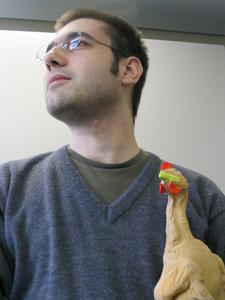
\includegraphics[height=.8\textheight]{fig/felipe1.jpg}
		\end{center}
	\end{frame}
%---------------------------------------------------------------------------------
\section{What is Goal Recognition?}

% \subsection{Motivation and Intuition}
	% \begin{frame}[c]\frametitle{Tentative Structure}
% 		\begin{itemize}
% 			\item Introduction to plan recognition (from Automated Planning)
% 			\item Goal recognition heuristics
% 			\item Hybrid goal recognition heuristics (ask Mor)
% 			\item Optimality monitoring and applications
% 			\item Recognizing plans using real-time video data
% 			\item Future work
% 		\end{itemize}
% 	\end{frame}

	\begin{frame}[c]\frametitle{What is it?}
		\begin{itemize}
			\item \textbf{Goal Recognition} is the task of recognizing agents' goal that explains a sequence of observations of its actions;
			\begin{itemize}
				\item Related to plan recognition, i.e. recognizing a \emph{top-level} action
				\item A specific form of the problem of abduction 
			\end{itemize}
			\item Roughly two types of approach:
			\begin{itemize}
				\item Plan-library based (\emph{classical} plan recognition)
				\item Domain-theory based (plan recognition as planning, or PRAP)
			\end{itemize}
		\end{itemize}
		\begin{center}
			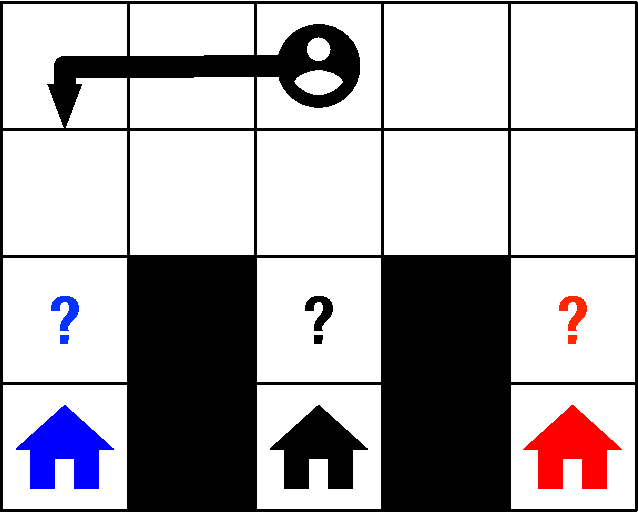
\includegraphics[width=.4\textwidth]{fig/gr-approaches/gr-concept.pdf}
		\end{center}
	\end{frame}

	\begin{frame}[c]\frametitle{Why do we need goal recognition?}
		\begin{itemize}
			\item Recognizing plans and goals of others is critical for meaningful interaction:
			\begin{itemize}
				\item important for humans/agents working in the same environment
				\item increasingly important as we build more intelligent systems
			\end{itemize}
			\begin{center}
				\includegraphics<1->[height=8em]{fig/intent-recognition-robot.jpg}
				\includegraphics<2>[height=8em]{fig/elderly-care.jpg}
				\includegraphics<3>[height=8em]{fig/creepy-care.jpg}
			\end{center}
			\item Overall area of Plan, Activity and Intent Recognition
			\begin{itemize}
				\item Activity recognition: recognizing meaningful activities from low-level sensor data
				\item Plan/Intent/Goal recognition: recognizing intentional higher-level sequences of activities 
			\end{itemize}
		\end{itemize}
	\end{frame}
	
	\begin{frame}[c]\frametitle{An example of Activity Recognition}
		% \animategraphics[loop,type=png,width=\linewidth]{2}{fig/egg-}{1}{4}
		\begin{center}
			\only<1>{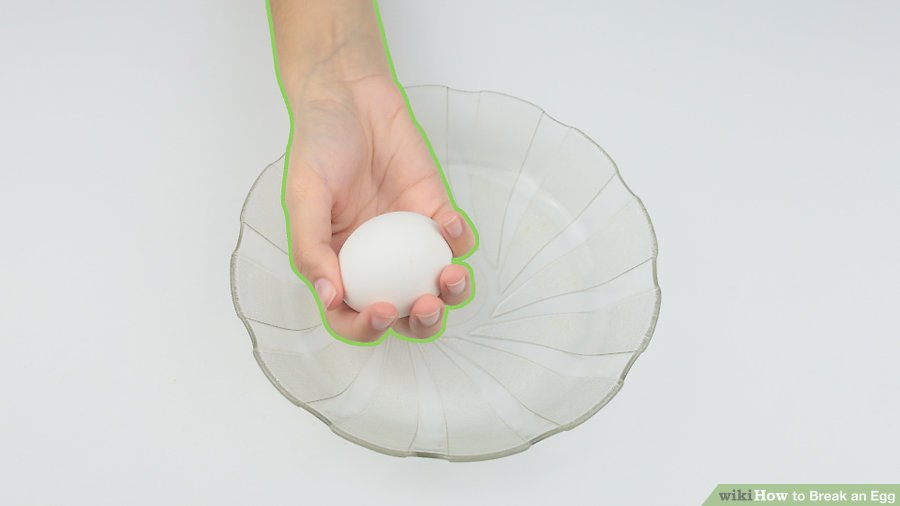
\includegraphics[width=.5\linewidth]{fig/egg-1.jpg}}
			\only<2>{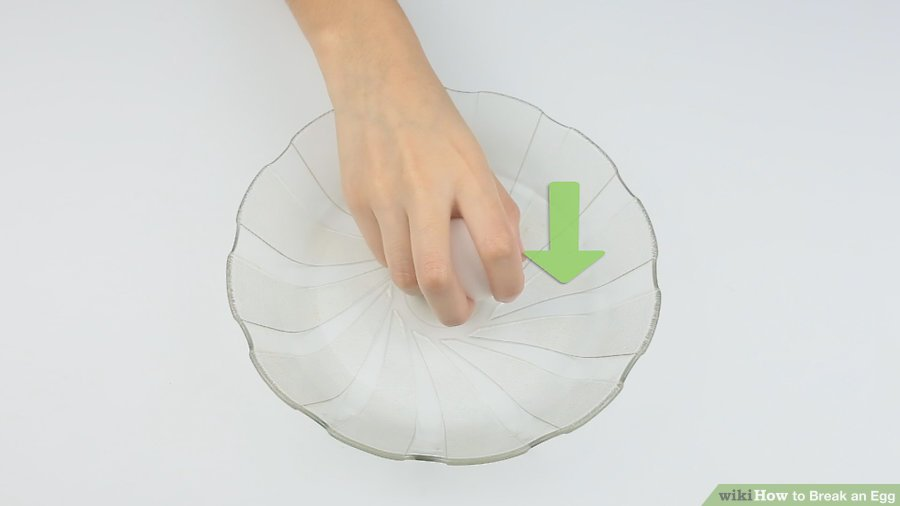
\includegraphics[width=.5\linewidth]{fig/egg-2.jpg}}
			\only<3>{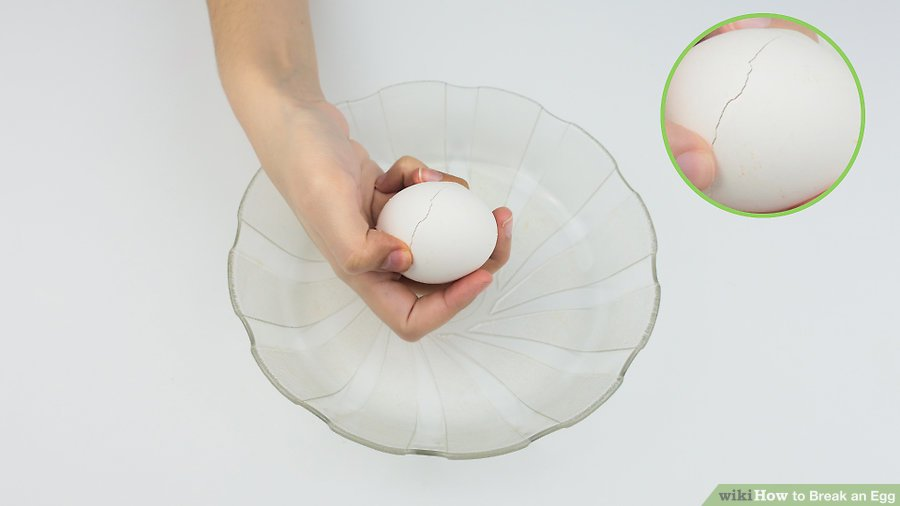
\includegraphics[width=.5\linewidth]{fig/egg-3.jpg}}
			\only<4>{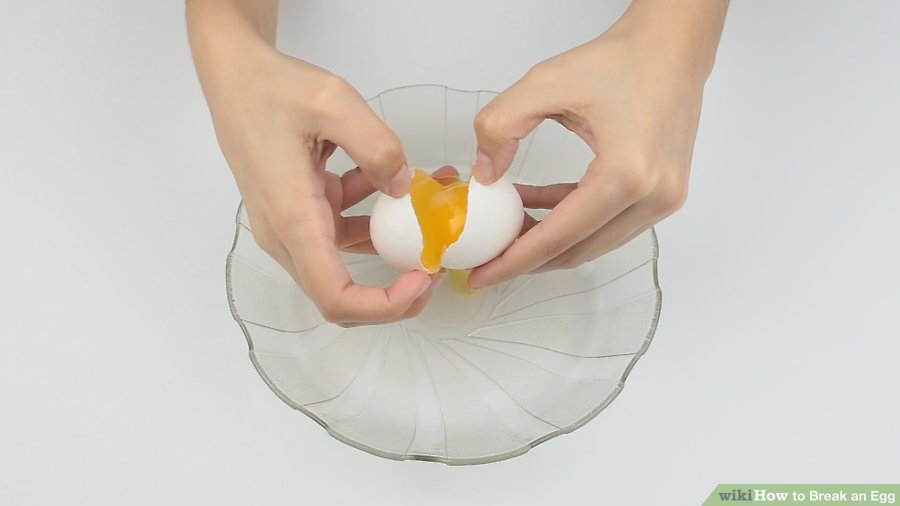
\includegraphics[width=.5\linewidth]{fig/egg-4.jpg} \\
			\texttt{breaking egg}
			}
		\end{center}
		% {\color{red} Complete this once I figure out how to include graphics}
		
	\end{frame}
	
	\begin{frame}[c]\frametitle{An Example of Goal/Plan Recognition}
		from Miquel Ramirez's thesis
		\begin{columns}
			\begin{column}{0.5\textwidth}
			    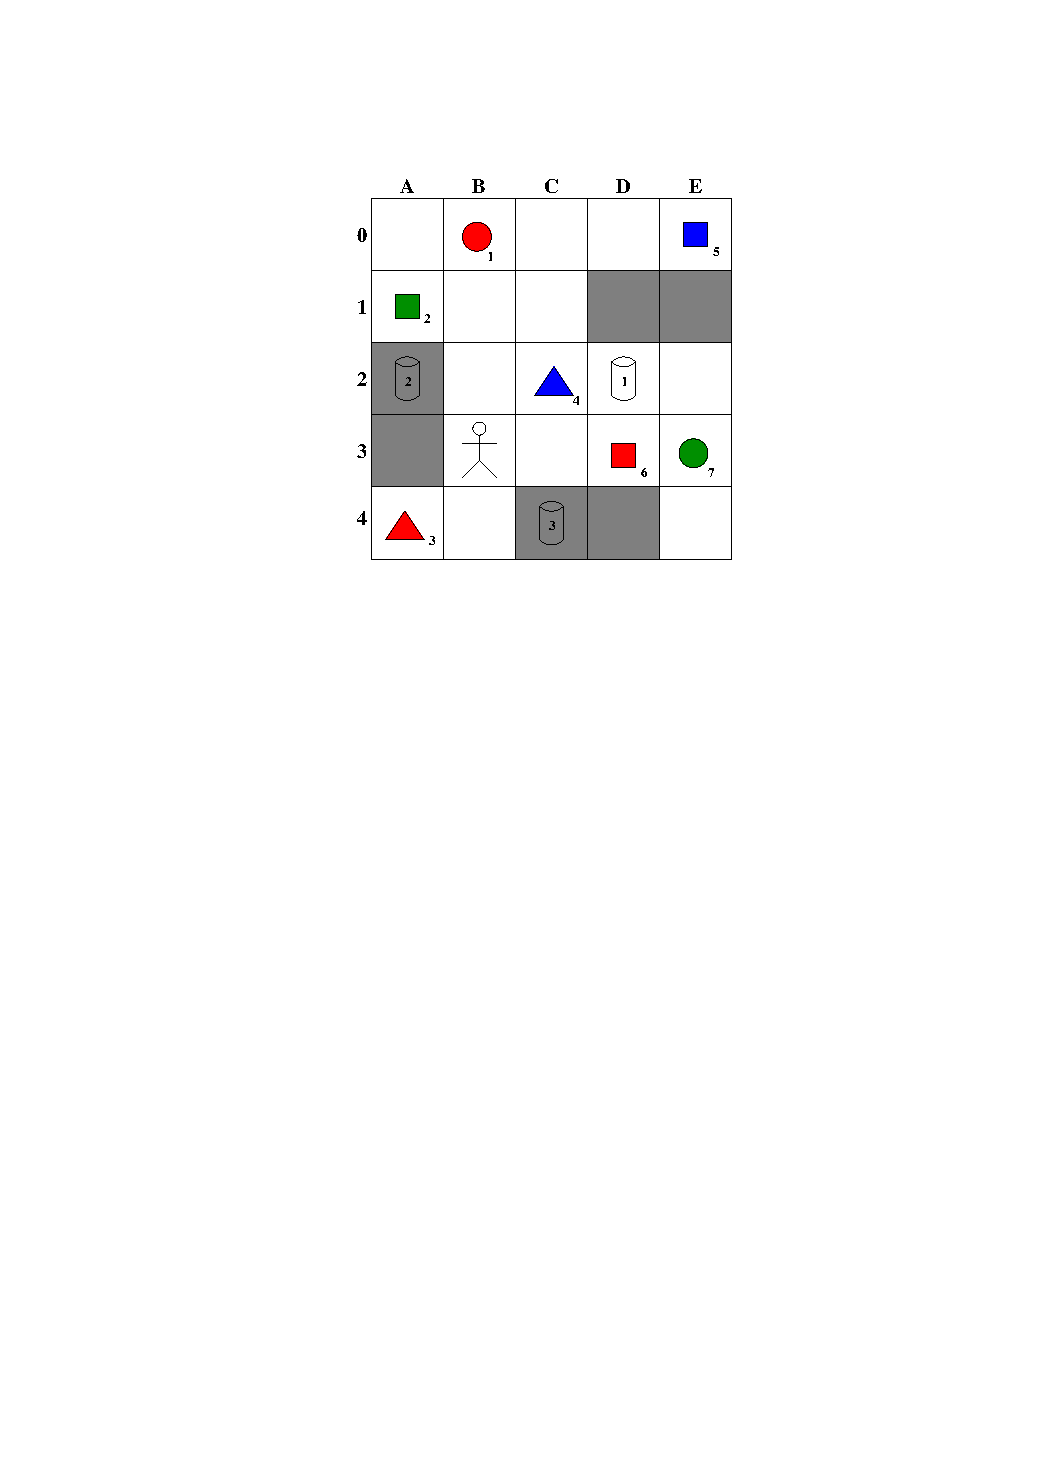
\includegraphics[width=.9\textwidth]{fig/roboschool-example.pdf}\\
				Wooden pieces $p_1,p_2, \dots p_n$\\
				Pieces have shapes and colors\\
				Bins $b_1, b_2, \dots, b_n$
			\end{column}
			\begin{column}{0.5\textwidth}
			\only<1>{
			The possible \textbf{goals} the trainer expected to pursue:
			\begin{enumerate}
				\item Store all triangles in $b_1$
				\item Store all spheres in $b_2$
				\item Store all cubes in $b_3$
				\item Store red objects in $b_2$
				\item Store green objects in $b_3$
				\item Store blue objects in $b_1$
			\end{enumerate}
			}
			\only<2>{
			One possible \emph{plan} for the trainer to achieve goal \#1 \\(store all triangles in $b_1$):
			\begin{enumerate}
				\item Walk from B3 into A4
				\item Pick $p_3$ up
				\item Walk from A4 into B3
				\item Walk from B3 into C2
				\item Pick $p_4$ up
				\item Throw $p_3$ into $b_1$
				\item Throw $p_4$ into $b_1$
			\end{enumerate}
			}
			\only<3->{
			If sensors miss 70\% of \emph{walk} actions and half \emph{pick} and \emph{drop} actions, we may only see:
			\begin{enumerate}
				\item Pick $p_3$ up
				\item Walk from A4 into B3
			\end{enumerate}
			}
			\only<4->{
			Here, we could deduce either goal \#1 or \#4 (store all red objects in $b_2$), as other tasks are less \emph{likely}.
			}
			\end{column}
		\end{columns}
	\end{frame}
	
	\begin{frame}[c]\frametitle{Flavors of Recognition Formalism}
		\begin{columns}
			\begin{column}[t]{0.5\textwidth}
				Plan Library
				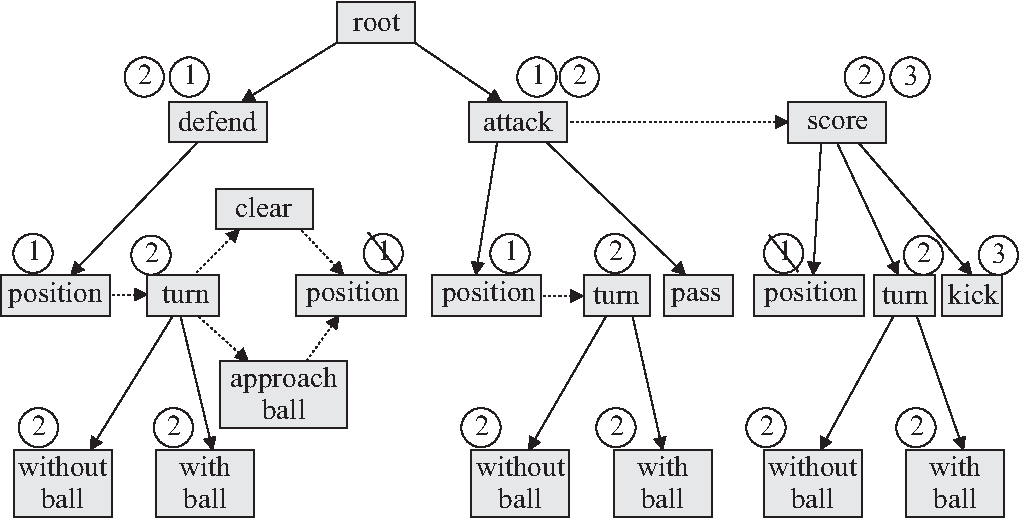
\includegraphics[width=\textwidth]{examples/fig_plan_library.pdf}
			\end{column}
			\begin{column}[t]{0.5\textwidth}
				Domain Theory (PRAP)
				\lstinputlisting[basicstyle=\fontsize{4}{4.5}\selectfont,language=LISP]{examples/easy_ipc_grid.pddl.txt}
			\end{column}
		\end{columns}
	\end{frame}
    
%---------------------------------------------------------------------------------
\if\masterclass1
\subsection{Formalism}

	\begin{frame}[c]\frametitle{Automated Planning}
		\begin{definition} [\textbf{Planning}]
			A planning instance is represented by a triple $\Pi = \langle \Xi, \mathcal{I}, G\rangle$, in which:
			\begin{itemize}
				\item $\Xi = \langle \Sigma, \mathcal{A} \rangle$ is the \textbf{domain definition}, and consists of a finite set of \textbf{facts} $\Sigma$ and a finite set of \textbf{actions} $\mathcal{A}$ (action costs typically 1);
				\item $\mathcal{I} \subseteq \Sigma$ and $G \subseteq \Sigma$ represent the \textbf{planning problem}, in which $\mathcal{I} \subseteq \Sigma$ is the \textbf{initial state}, and $G \subseteq \Sigma$ is the \textbf{goal state}.
			\end{itemize}
		\end{definition}
		\begin{itemize}
			\item Actions $a \in \mathcal{A}$ are tuples $a = \langle \mathit{pre}(a), \mathit{eff}(a), \mathit{cost}(a) \rangle$
			\item Facts $\Sigma$ can be modeled in a variety of ways:
			\begin{itemize}
				\item As a logic language (restricted FOL): \\states are truth assignments
				\item As a set of variables $\mathcal{V}$ with finite domains: \\states are variable assignments
			\end{itemize}
			 %\todo{Complete this in a new slide}
		\end{itemize}
	\end{frame}

	\begin{frame}[c]\frametitle{Roboschool}
		{\color{red} Add Roboschool formalization}
	\end{frame}

    \begin{frame}[c]\frametitle{Goal Recognition Problem}
		\begin{definition}[\textbf{Goal Recognition Problem}]
			A goal recognition problem is a tuple $P = \langle \Xi, \mathcal{I}, \mathcal{G}, \mathbf{O} \rangle$, where:
       	\begin{itemize}
       		\item $\Xi = \langle \Sigma, \mathcal{A} \rangle$ is the domain definition (facts and actions) ;
       		\item $\mathcal{I} \subseteq \Sigma$ is the initial state;
       		\item $\mathcal{G}$ s.t. $\forall{G \in \mathcal{G}}, G \subseteq \Sigma$ is a set of candidate goals (with an assumed hidden goal $G$); and
       		\item $\mathbf{O}$ is a sequence $\langle o_1, \dots o_n \rangle$ of observations, where $o_i \in \mathcal{A}$
       	\end{itemize}
       	\end{definition}
        
        \begin{itemize}
        	\item The solution for a goal recognition problem is the hidden goal $G \in \mathcal{G}$ that is most consistent with observation sequence $O$.
        	\item Caveat: we may have other representations for the observations
        	\item This is what I will refer to as PRAP
        \end{itemize}
    \end{frame}	
 
	\begin{frame}[c]\frametitle{Plan Recognition Problem}
		\begin{definition}[Plan Recognition Problem]
			\todo{Figure out formalization}
		\end{definition}
		
		\begin{itemize}
			\item Requires a lot more domain knowledge
			\item This is what I will refer to as classical plan recognition 
		\end{itemize}
	\end{frame}
	
	\begin{frame}[c]\frametitle{Roboschool}
		{\color{red} Add Roboschool problem for master class}
	\end{frame}
	
	\begin{frame}[c]\frametitle{Observations}
		Often, this means Observed Actions\\
        This observation sequence can be either \textbf{partial} or \textbf{full}.\\
            \todo{Observations as actions, and states, animation}
	\end{frame}
\fi

%---------------------------------------------------------------------------------

\section{A Canned History of Current Approaches}

% \begin{frame}[c]{Goal Recognition using Planning Formalisms}
% 	\begin{itemize}
% 		\item Ramirez and Geffner
% 		\item E-Martín
% 		\item Sohrabi
% 		\item Pereira and Meneguzzi
% 	\end{itemize}
% \end{frame}

\begin{frame}[c,allowframebreaks]\frametitle{Goal Recognition using Planning Domains}
	
	Ramirez and Geffner (2009 and 2010)
	\begin{itemize}
		\item First approaches to goal recognition: Plan Recognition as Planning (PRAP)
		\item Probabilistic model aims to compute $P(G \mid O)$
		\item Following Bayes Rule $P(G \mid O) = \alpha P(O \mid G) P(G)$
		\item Given $P(G)$ as a prior, key bottleneck is computing $P(O \mid G)$
		% \begin{itemize}
% 			\item Compute $P(O \mid G)$ in terms of a cost difference $c(G,O) - c(G,\bar{O})$
% 			\item Computational cost is \textbf{two planner calls per goal hypothesis}
% 			\item For online recognition: two planner calls per goal hypothesis \textbf{per observation}
% 		\end{itemize}
% 		\item Some conclusions challenged for path planning domains\\ (Masters and Sardina 2017)
	\end{itemize}
	\begin{columns}
		\begin{column}{.5\textwidth}
			\begin{itemize}
				\normalsize
				\item Compute $P(O \mid G)$ in terms of a cost difference $c(G,O) - c(G,\bar{O})$
				\item Costs \textbf{two planner calls per goal hypothesis}
				% \item For online recognition: two planner calls per goal hypothesis
			\end{itemize}
		\end{column}
		\begin{column}{.5\textwidth}
			\begin{center}
				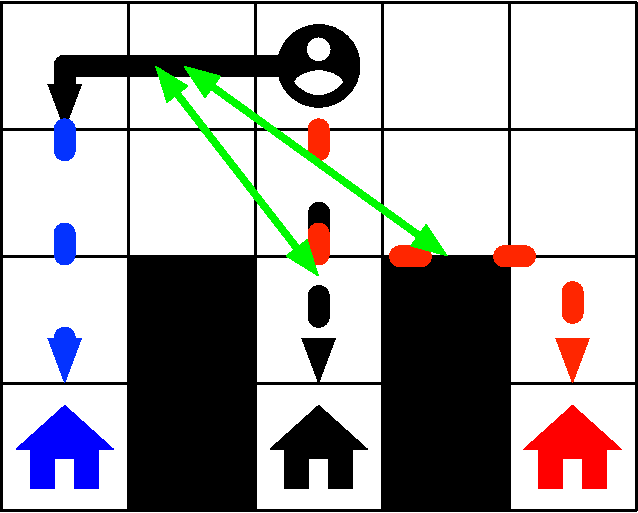
\includegraphics[width=12em]{fig/gr-approaches/gr-ramirez.pdf}
			\end{center}
		\end{column}
	\end{columns}
	% \framebreak
	%
	% E-Martín et al. (2015)
	%
	% \framebreak
	%
	% Sohrabi et al. (2017)
\end{frame}

\begin{frame}[c]{Goal Recognition using Planning Heuristics}
	Pereira, Oren and Meneguzzi (2017):
   	\begin{itemize}
		\item \textbf{Obviate the need to execute a planner multiple times} for recognizing goals; and
		\item Novel goal recognition heuristics that use \textbf{planning landmarks}.
		% \item We evaluate our approaches against the fastest and most accurate approach of Ramírez and Geffner ({\footnotesize Plan Recognition as Planning. IJCAI, 2009}) over \textbf{15 planning domains};
		\item \textbf{More accurate} and \textbf{orders of magnitude faster} than all previous approaches.
	\end{itemize}
	\begin{columns}
		\begin{column}{.5\textwidth}
			Planning Landmarks:
			\begin{itemize}
				\item Are \textbf{necessary conditions} for any valid plan
				\item Theoretical cost of computation is the same as planning
			\end{itemize}
		\end{column}
		\begin{column}{.5\textwidth}
			\begin{center}
				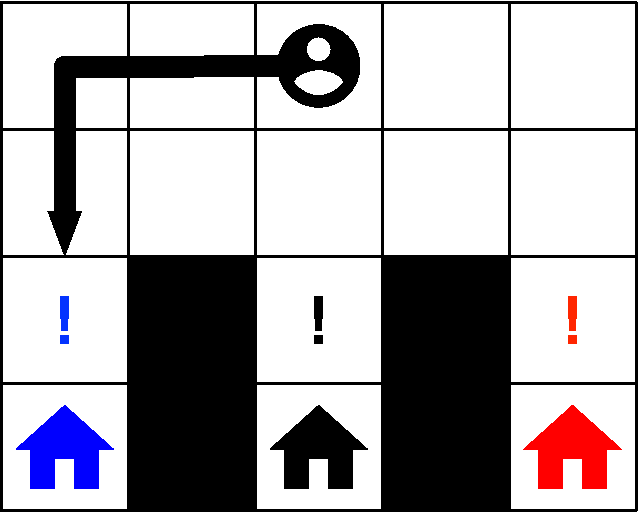
\includegraphics[width=12em]{fig/gr-approaches/gr-landmarks.pdf}
			\end{center}
		\end{column}
	\end{columns}
\end{frame}

\begin{frame}[c]{Goal Recognition using Operator-Counting Constraints}
	Meneguzzi, Pereira and Pereira (2020):
   	\begin{itemize}
		\item Use \textbf{operator counting} heuristic information for recognizing goals; and
		\item Operator counts and LP constraints cope explicitly with noisy observations.
		% \item We evaluate our approaches against the fastest and most accurate approach of Ramírez and Geffner ({\footnotesize Plan Recognition as Planning. IJCAI, 2009}) over \textbf{15 planning domains};
	\end{itemize}
	\begin{columns}
		\begin{column}{.5\textwidth}
			Key advantages:
			\begin{itemize}
				\item \textbf{More accurate} than all previous approaches; and
				\item Provides an \textbf{extensible framework} for further goal recognition work.
			\end{itemize}
		\end{column}
		\begin{column}{.5\textwidth}
			\begin{center}
				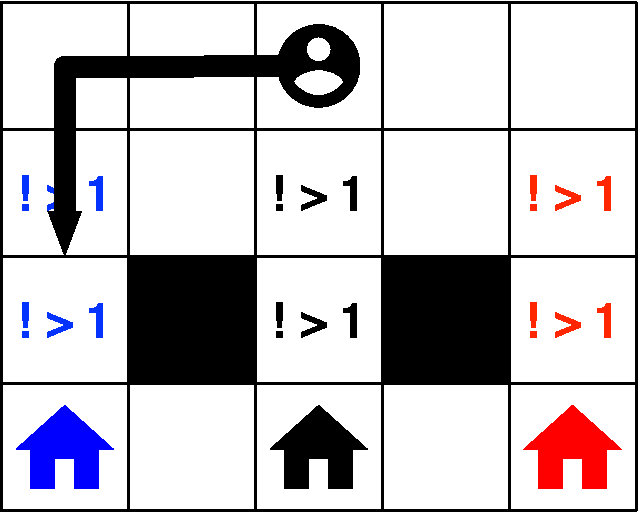
\includegraphics[width=12em]{fig/gr-approaches/gr-operator-counting.pdf}
			\end{center}
		\end{column}
	\end{columns}
\end{frame}


\section{Goal Recognition using Real World Data}

{
\usebackgroundtemplate{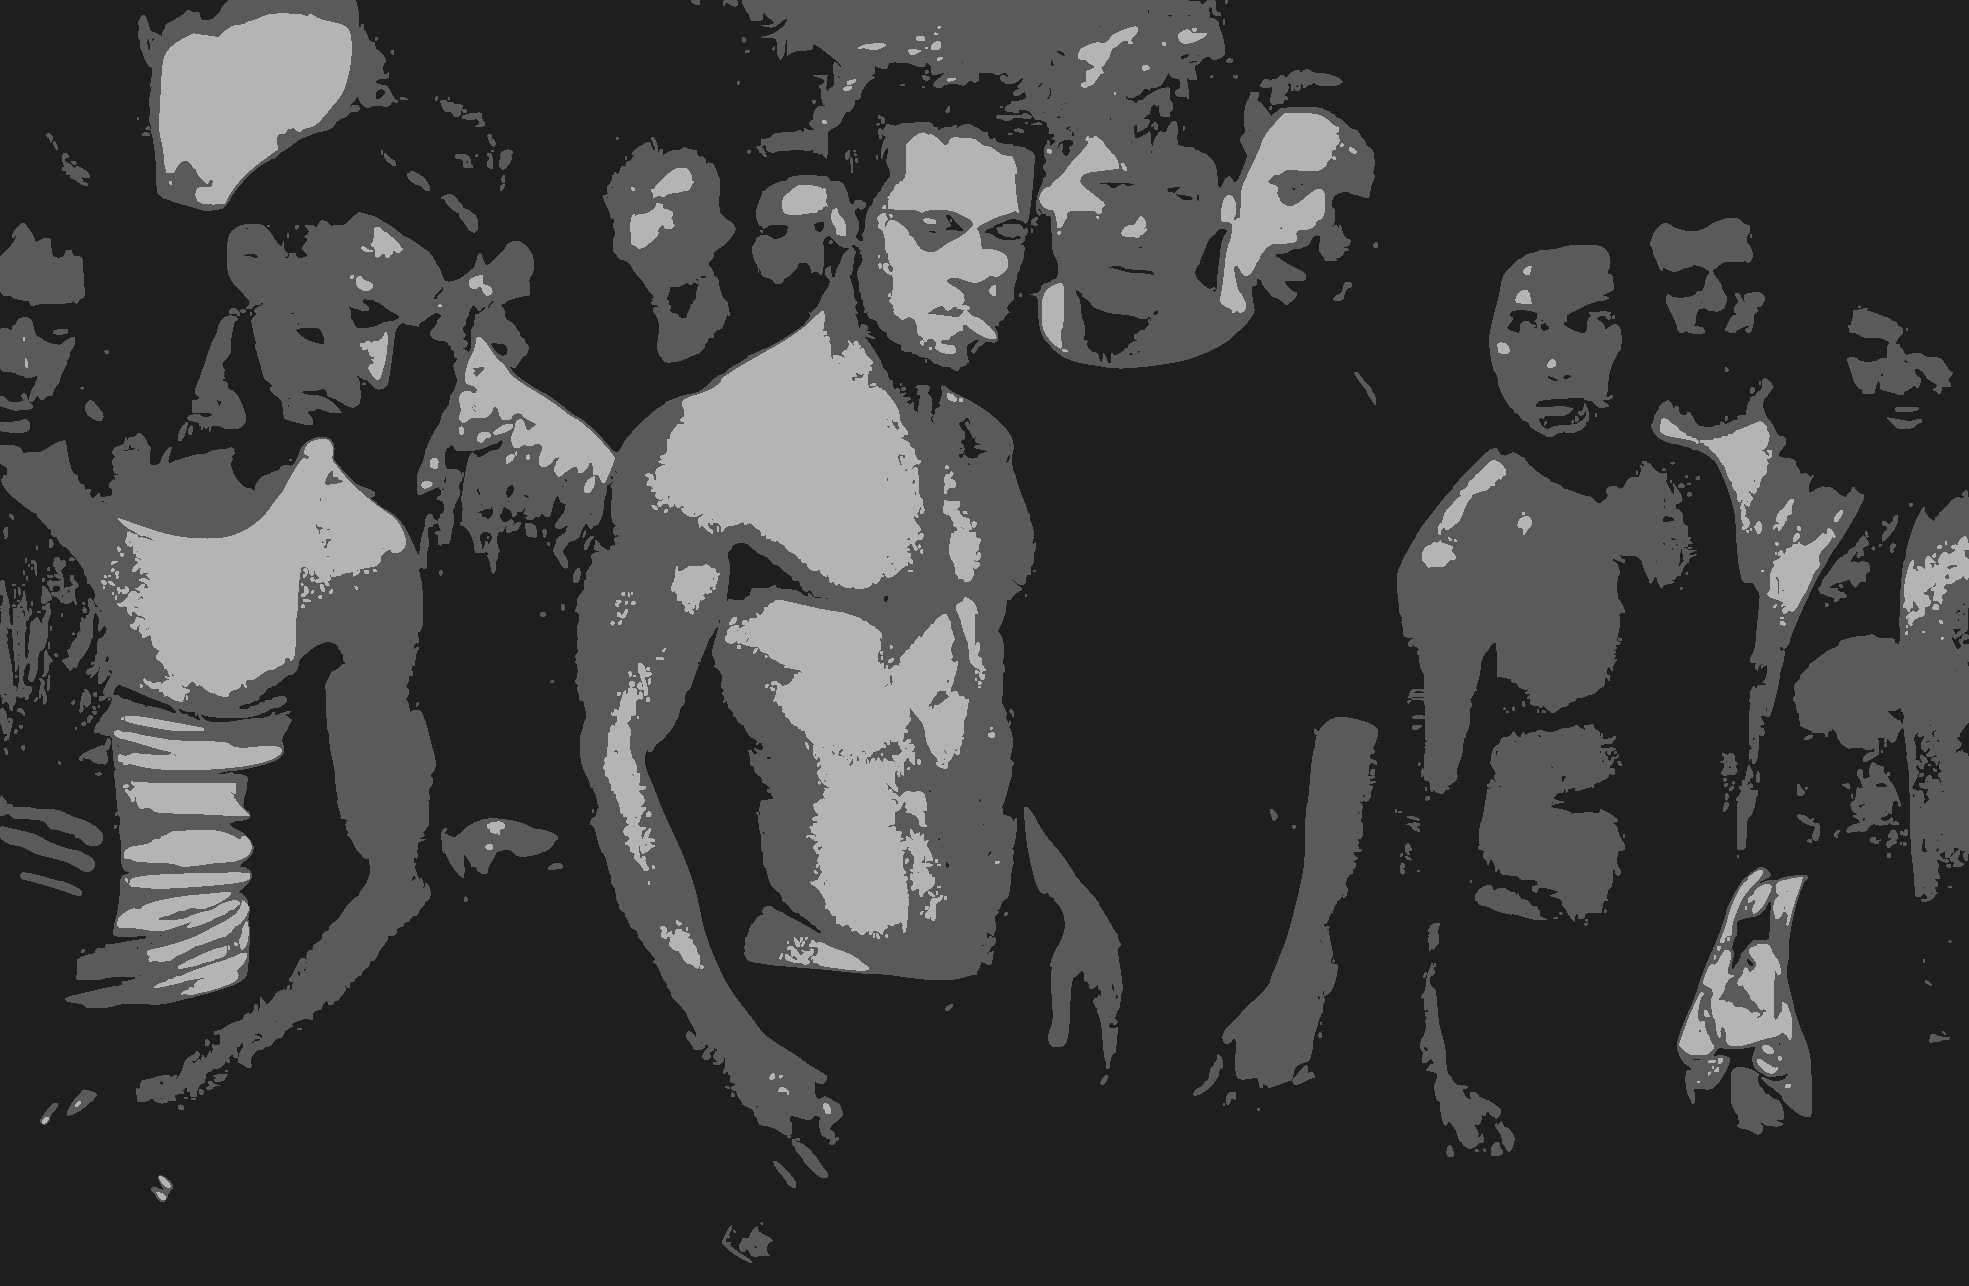
\includegraphics[width=\paperwidth]{fig/fightclub.pdf}}%
\begin{frame}[b]{Warning}
\begin{itemize} \Large
	\item \color{white} I will now talk about Machine Learning, \\ but I do not buy into the hype
	\item<2-> ML Inverse Fight Club (James Mickens)
	\begin{enumerate} \color{white} \large
		\item<3-> First Rule: You must talk about fight club
		\item<4-> Second Rule: Let's not fight because we all agree that ML is awesome
	\end{enumerate}
\end{itemize}
\vspace*{2em}
\end{frame}
}

\begin{frame}[c]{Where can we use real-world data?}
	\begin{columns}
		\begin{column}{0.5\textwidth}
			\begin{itemize}
				\item Domain description: \\What we want to recognize?
				\begin{itemize}
					\item Environment domain
					\item Subject preferences
				\end{itemize}
				\item Goal Recognition: \\How do we deal with the observations?
				\begin{itemize}
					\item Generate observations from raw data
					\item Cope with noise from observations
				\end{itemize}
			\end{itemize}
		\end{column}
		\begin{column}{0.5\textwidth}
			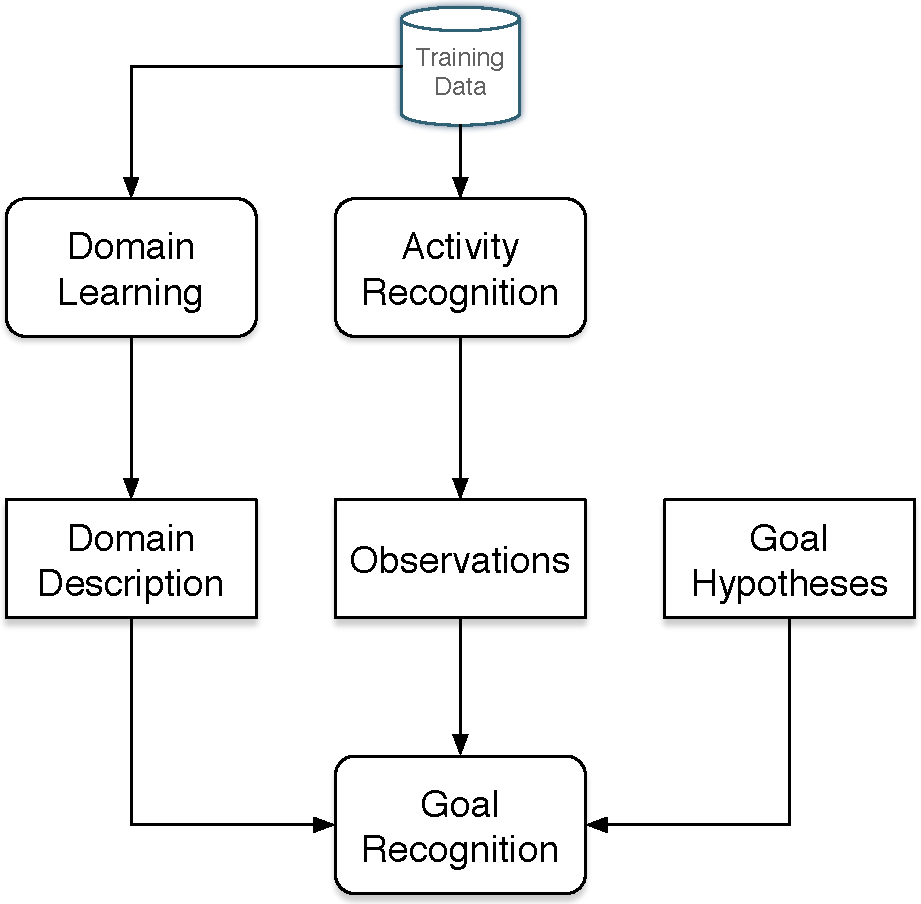
\includegraphics[width=.9\textwidth]{fig/gr-learning.pdf}	
		\end{column}
	\end{columns}
\end{frame}

\begin{frame}[c]{Limitations of previous approaches}
	\begin{itemize}
		\item Domain Knowledge:
		\begin{itemize}
			\item Must be engineered by humans
			\item Must be \textbf{perfect}
		\end{itemize}
		\item Observations:
		\begin{itemize}
			\item Must be ``well-behaved'' in some sense
			\item Do not use raw, real-world data
		\end{itemize}
	\end{itemize}
\end{frame}


{
\usebackgroundtemplate{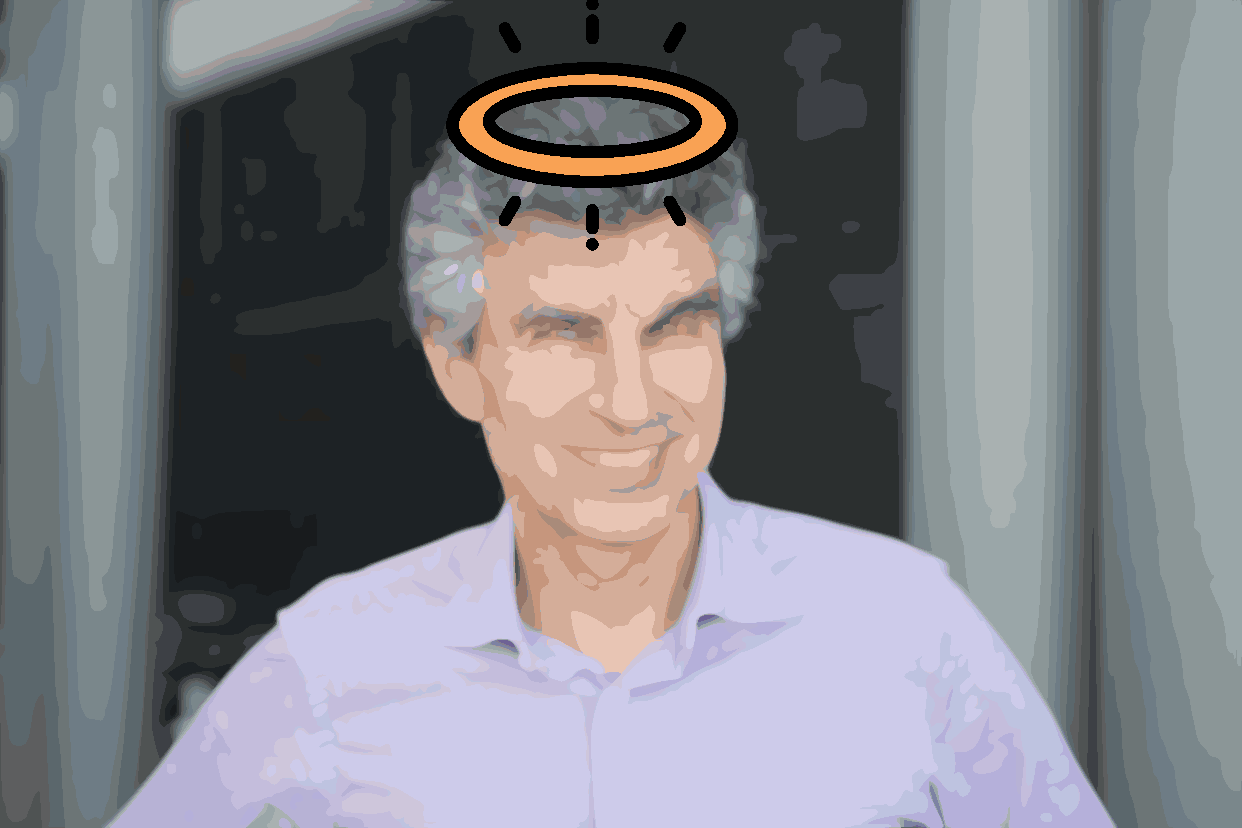
\includegraphics[width=\paperwidth]{fig/bengio.pdf}}%
\begin{frame}[b]{Machine Learning Again}
	\begin{itemize} \Large
		\item \color{white} Do I hate machine learning then?
		\item<2-> No, I love it! 
		\begin{enumerate} \color{white} \large
			\item<3-> If you are doing any unstructured data input
			\item<4-> If you want to impress your friends or peddle for money
		\end{enumerate}
	\end{itemize}
	\vspace*{3em}
\end{frame}
}

% \begin{frame}[t]{Now let's talk politics}
% 	\Huge Who should win the next election? \\[4em]
%
%
% 	\onslide<2->{
%
% 		% \vspace{10em}
% 		\begin{center}
% 			\normalsize Just kidding, let's go back to our talk
% 		\end{center}
% 	}
%
%
% \end{frame}

\begin{frame}[c]{How do we try to solve this?}
	\begin{itemize}
		\item To Generate Symbolic Observations:
		\begin{itemize}
			\item ML to map raw data into recognition algorithm
			\item ML algorithms to generate \textbf{symbolic observations}
		\end{itemize}
		\item Obtain Domain Knowledge:
		\begin{itemize}
			\item Cope with expected noisy observations relaxing the domain model
			\item Learn PDDL representations from image data
			\item Learn \textbf{Nominal Models} from raw data
		\end{itemize}
		\item To work on both problems simultaneously
		\begin{itemize}
			\item Hybrid engineering/learning of PDDL representations 
		\end{itemize}
	\end{itemize}
\end{frame}

\subsection{Plan Recognition using Video Data}
% \begin{frame}[c]\frametitle{Plan Recognition using Video Data}
% 	Get slides from Roger
% \end{frame}

\begin{frame}[c]
	\begin{center}
		\Large{Plan Recognition using Video Data}
	\end{center}
\end{frame}

\begin{frame}[c]\frametitle{Plan Recognition using Video Data}
	% \begin{itemize}
%    		\item \textbf{Plan recognition}
%    		\begin{itemize}
% 				\item Task of recognizing the plan (i.e., the sequence of actions) the observed agent is following in order to achieve his intention %(Sadri, 2012)
% 	    \end{itemize}
% 		\item \textbf{Activity recognition}
% 			\begin{itemize}
% 				\item The task of recognizing the independent set of actions that generates an interpretation to the movement that is being performed (Poppe,~2010)
% 				\item This is particularly challenging in the real physical world
% 			 \end{itemize}
% 	\end{itemize}
	\begin{columns}
		\begin{column}{.7\textwidth}
			\begin{itemize}
				\item Most research focuses on activity and plan recognition separately;
				\item We develop a hybrid approach that comprises both;
				\item The approach infers, from a set of candidate plans, which plan a human subject is pursuing based exclusively on fixed-camera video.
			\end{itemize}
		\end{column}
		\begin{column}{.3\textwidth}
			\begin{center}
				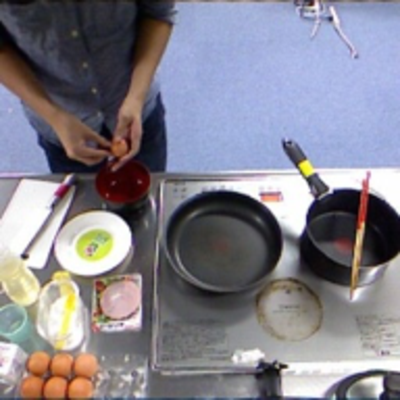
\includegraphics[width=9em]{fig/computer-vision-eggs.pdf}
			\end{center}
		\end{column}
	\end{columns}
\end{frame}

\begin{frame}[c]\frametitle{A Hybrid Architecture for Activity and Plan Recognition}
   	\begin{itemize}
   		\item \textbf{Conceptually divided in two main parts}
   		\begin{itemize}
				\item CNN-based activity recognition (CNN)\footnote{That's us!}
                \item CNN-backed symbolic plan recognition (SBR)\footnote{Not our work: Avrahami-Zilberbrand and Kaminka. Fast and Complete Symbolic Plan Recognition. IJCAI 2005}
	    \end{itemize}
	\end{itemize}
	\begin{center}
		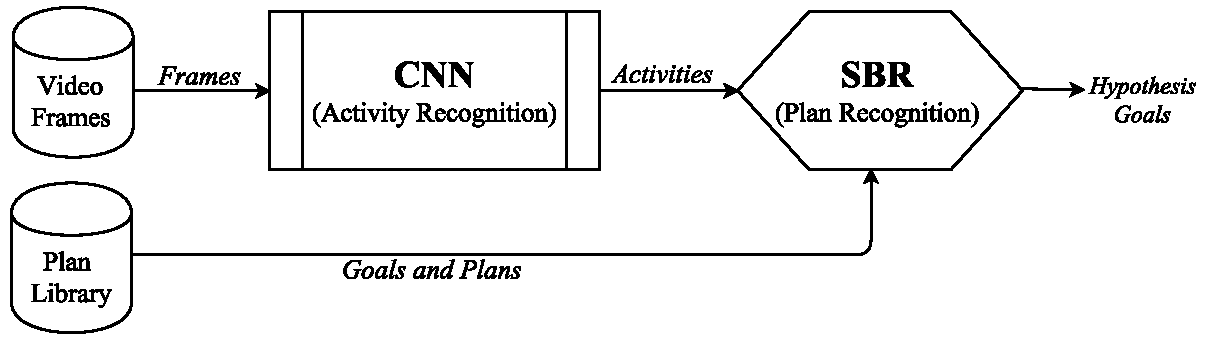
\includegraphics[width=0.8\linewidth]{fig/pipeline.pdf}
	\end{center}
\end{frame}

\if\masterclass1
\begin{frame}[c]\frametitle{CNN-based Activity Recognition}
   	\begin{itemize}
   		\item \textbf{Convolutional Neural Network}
   		\begin{itemize}
   		    \item Architecture: GoogLeNet
			\item 22-layer deep network based on the Inception module
            \item Input images: 224x224 (3 channels: RGB)
            \item Output classes: 9 (activities)
	    \end{itemize}
		
	\end{itemize}
\end{frame}

\begin{frame}{CNN-backed Symbolic Plan Recognition}
   	\begin{itemize}
   		\item \textbf{Symbolic Behavior Recognition (SBR)}
   		\begin{itemize}
				\item A plan recognition approach that takes as input a plan library and a sequence of observations
                \item Feature decision tree (FDT) maps observable features to plan-steps in a plan library
                \item SBR returns set of hypotheses plans such that each hypothesis represents a plan that achieves a top-level goal in a plan library
	    \end{itemize}
		\begin{center}
			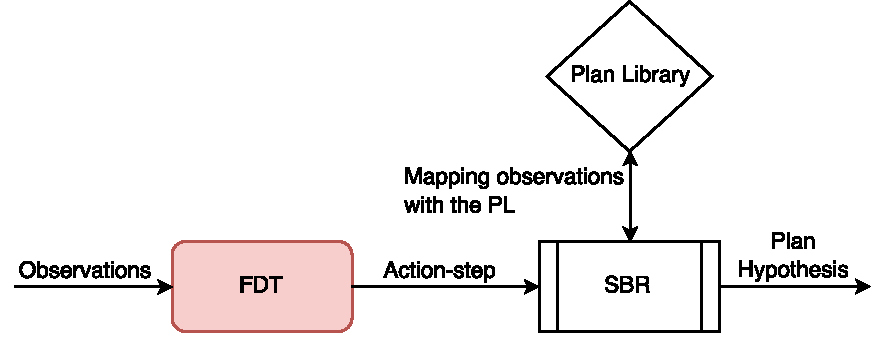
\includegraphics[width=0.7\linewidth]{fig/fdt.pdf}
		\end{center}
	\end{itemize}
\end{frame}

\begin{frame}[c]\frametitle{CNN-backed Symbolic Plan Recognition}
   	\begin{itemize}
   		\item \textbf{Our Symbolic Behavior Recognition}
   		\begin{itemize}
				\item We modify the SBR and replace the FDT with the CNN-backed Activity Recognition
                \item The CNN-backed Activity Recognition maps frames directly into nodes (activities) in the plan library used by SBR to compute sequential consistency of plan steps
	    \end{itemize}
		\begin{center}
			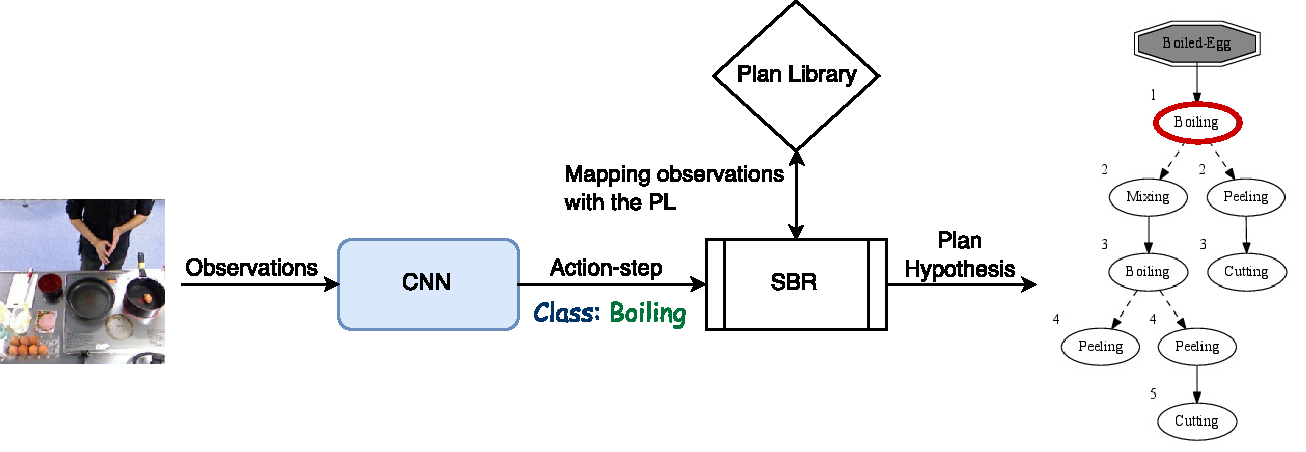
\includegraphics[width=0.9\linewidth]{fig/sbr.pdf}
		\end{center}
	\end{itemize}
\end{frame}
\fi

% \begin{frame}{Experiments: Dataset}
%    	\begin{itemize}
%    		\item ICPR 2012 Kitchen Scene Context based Gesture Recognition dataset (KSCGR)%\footnote{http://www.murase.m.is.nagoya-u.ac.jp/KSCGR/}
% 	    \item \textbf{5 recipes for cooking eggs in Japan}
%    		\begin{itemize}
% 				\item Ham and Eggs, Omelet, Scrambled-Egg, Boiled-Egg and Kinshi-Tamago
% 				\item Each recipe is performed by 7 subjects \\(5 in training set, 2 in testing set)
% 	    \end{itemize}
% 	    \item \textbf{9 cooking activities within the dataset}
%    		\begin{itemize}
% 				\item Breaking, mixing, baking, turning, cutting, boiling, seasoning, peeling, and none
% 	    \end{itemize}
% 		\begin{figure}[here]
% 			\centering
% 			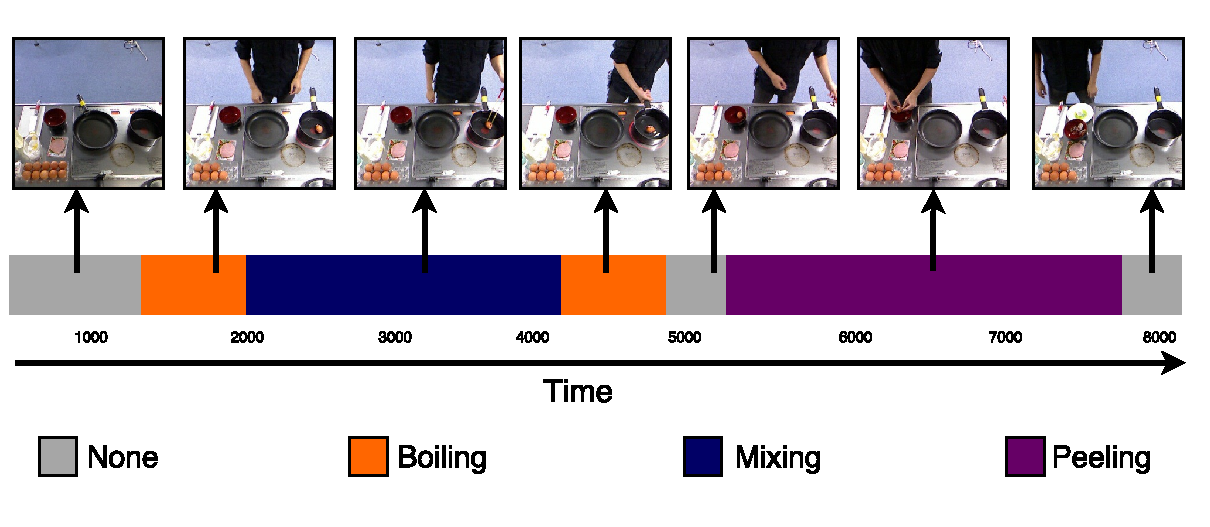
\includegraphics[width=0.7\linewidth]{fig/egg-dataset.pdf}
% 		\end{figure}
% 	\end{itemize}
% \end{frame}

\begin{frame}[c]{How are we doing so far?}
	\begin{itemize}
		\item To Generate Symbolic Observations:
		\begin{itemize}
			\item ML to map raw data into a recognition algorithm {\Large \color{red} \checkmark}
			\item ML algorithms to generate \textbf{symbolic observations}
		\end{itemize}
		\item Obtain Domain Knowledge:
		\begin{itemize}
			\item Cope with expected noisy observations relaxing the domain model
			\item Learn PDDL representations from image data
			\item Learn \textbf{Nominal Models} from raw data
		\end{itemize}
		\item To work on both problem simultaneously
		\begin{itemize}
			\item Hybrid engineering/learning of PDDL representations 
		\end{itemize}
	\end{itemize}
\end{frame}

\subsection{Goal Recognition in Incomplete Domains}

\begin{frame}[c]
	\begin{center}
		\Large{Goal Recognition in Incomplete Domains}
	\end{center}
\end{frame}

	\begin{frame}[c]{What is an Incomplete Domain?}
		In a nutshell: \\
			It is a STRIPS/PDDL domain that allows me to state that some preconditions/effects \textbf{may or may not} be there!
		% Add figure of invisible man
	\end{frame}
	
    \begin{frame}{Why use Incomplete Domains?}
       	\begin{itemize}
			% Sometimes we do not have full knowlegde about the dynamics of the domain model.
			\item A \textbf{step forward} to \textbf{more realistic settings}; and
			
			% Even having a domain expert, sometimes it is hard to formalize a domain model completly.
       		\item The \textbf{lack of domain knowledge}, human-error, and etc.
			\begin{figure}[]
			 	\centering
			 	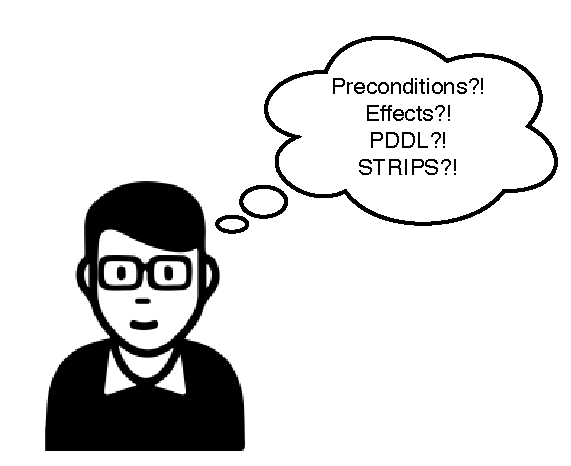
\includegraphics[width=0.8\linewidth]{fig/nerd-incomplete_domain.pdf}
			\end{figure}
		\end{itemize}
    \end{frame}
	
    \begin{frame}{Background: Incomplete STRIPS Domain Models}
		\begin{definition} [\textbf{Incomplete STRIPS Domain Model\footnote{\tiny \it Weber and Bryce, Planning and Acting in Incomplete Domain Models. ICAPS, 2011.}}]
			An incomplete STRIPS domain model is a tuple $\incp{D} = \langle \mathcal{R}, \incp{O} \rangle$, where:
			\begin{itemize}
				\item $\mathcal{R}$ is a set of predicates with typed variables;
				\item $\incp{O}$ is a set of incomplete operators. An operator $\inc{op} \in \incp{O}$ defines: 
				\begin{itemize}
					\item $pre(\inc{op}) \subseteq \mathcal{R}$ as a set of known preconditions;
					\item<2-> $\widetilde{pre}(\inc{op}) \subseteq \mathcal{R}$ as a set of \textbf{possible preconditions};
					\item $add(\inc{op}) \subseteq \mathcal{R}$ as a set of known add effects;
					\item<2-> $\widetilde{add}(\inc{op}) \subseteq \mathcal{R}$ as a set of \textbf{possible add effects};
					\item $del(\inc{op}) \subseteq \mathcal{R}$ as a set of known delete effects;
					\item<2-> $\widetilde{del}(\inc{op}) \subseteq \mathcal{R}$ as a set of \textbf{possible delete effects};
				\end{itemize}
			\end{itemize}
		\end{definition}
    \end{frame}

    % \begin{frame}{Problem Overview (1 of 2)}
%        	\begin{itemize}
%        		\item We assume that the \textbf{recognizer} (\textbf{observer}) has an \textbf{incomplete domain model} while the \textbf{observed agent} is planning and acting in the environment with a \textbf{complete domain model};
% 			\vspace{2mm}
% 			\item We \textbf{do not change (or improve)} the incomplete domain model for recognizing goals;
% 		\end{itemize}
%     \end{frame}
%
%     \begin{frame}{Problem Overview (2 of 2)}
% 		\begin{figure}[]
% 		 	\centering
% 		 	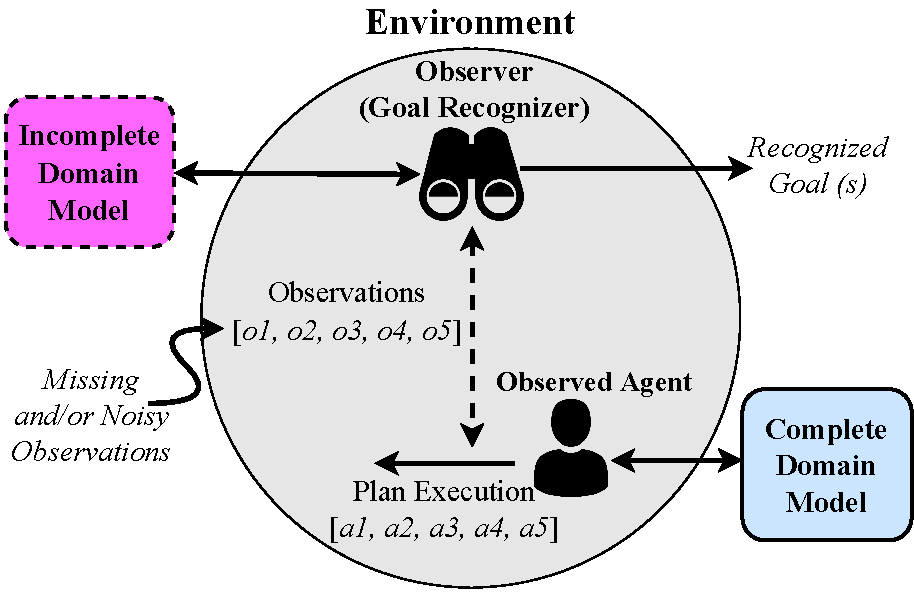
\includegraphics[width=0.9\linewidth]{fig/GoalRecognition-IncompleteDomains-Big.pdf}
% 		\end{figure}
%     \end{frame}
	
    \begin{frame}{Problem Overview}
		\begin{figure}[]
		 	\centering
		 	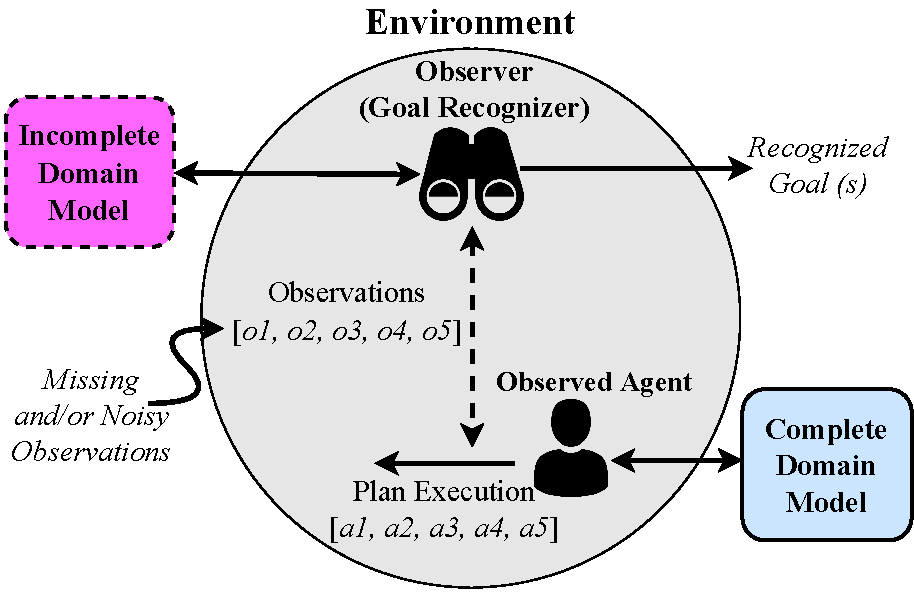
\includegraphics[width=0.9\linewidth]{fig/GoalRecognition-IncompleteDomains-Big.pdf}
		\end{figure}
    \end{frame}

\begin{frame}[c]{How are we doing so far?}
	\begin{itemize}
		\item To Generate Symbolic Observations:
		\begin{itemize}
			\item ML to map raw data into a recognition algorithm {\Large \checkmark}
			\item ML algorithms to generate \textbf{symbolic observations}
		\end{itemize}
		\item Obtain Domain Knowledge:
		\begin{itemize}
			\item Cope with expected noisy observations relaxing the domain model {\Large \color{red} \checkmark}
			\item Learn PDDL representations from image data
			\item Learn \textbf{Nominal Models} from raw data
		\end{itemize}
		\item To work on both problem simultaneously
		\begin{itemize}
			\item Hybrid engineering/learning of PDDL representations 
		\end{itemize}
	\end{itemize}
\end{frame}

\subsection{Plan Recognition in Latent Space}

\begin{frame}[c]
	\begin{center}
		\Large{Plan Recognition in Latent Space}
	\end{center}
\end{frame}

\begin{frame}[c]{Motivation}
	\begin{itemize}
		\item Goal and Plan Recognition depend on high-quality domain engineering
		\begin{itemize}
			\item PDDL domain theory for PRAP
			\item Plan Library for traditional PR
		\end{itemize}
		\item We would like to obviate the need for most domain engineering
		\begin{itemize}
			\item Learn domain models directly from raw data
			\item Recognize goals using raw data as observations
		\end{itemize}
	\end{itemize}
\end{frame}

\begin{frame}[c]{Inspiration: LatPlanner\footnote{\tiny Not our Work: Asai and Fukunaga. Classical Planning in Deep Latent Space: Bridging the Subsymbolic-Symbolic Boundary, AAAI, 2018}}
	\begin{center}
		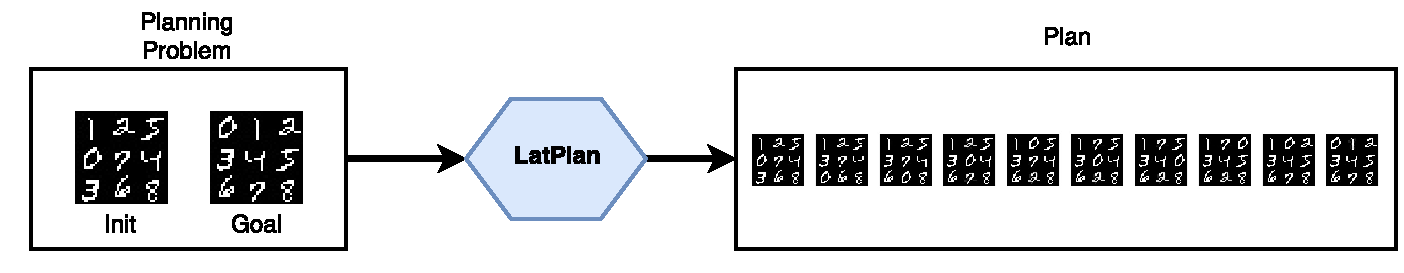
\includegraphics[width=10cm]{fig/latplan.pdf}
	\end{center}
\end{frame}

\begin{frame}[c]{Variational Autoencoders}
	\begin{itemize}
		\item Autoencoders are a specific type of Neural Network intended to learn representations
		\item Consists of three key parts
		\begin{itemize}
			\item Encoder network
			\item Latent layer (the middle layer)
			\item Decoder network
		\end{itemize}
		\item Trained in an unsupervised manner
		\item Variational Autoencoders force the the encoder network to generate latent vectors following some distribution \\(typically a unit-gaussian one)
	\end{itemize}
	
	\begin{center}
		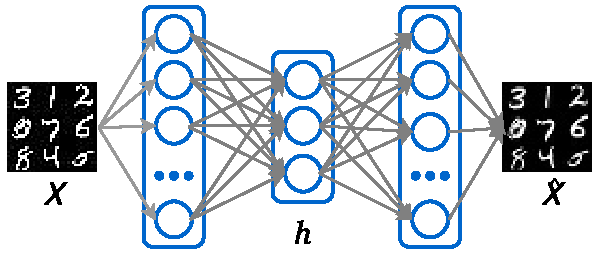
\includegraphics[width=5cm]{fig/autoencoder.pdf}
	\end{center}
\end{frame}


\begin{frame}[c]{Gumbel-softmax autoencoders and planning}
	\begin{itemize}
		\item Planners view states as sets of logical propositions (i.e. binary vectors)
		\item We would like to be able to learn state representations from raw data
		\item We force an autoencoder to have a categorial distribution in the latent layer:
		\begin{itemize}
			\item Gumbel-softmax activation can be annealed into a categorical distribution
			\item Latent layer now correspond to \textbf{logic bits}
			\item Can learn a PDDL transition function from pairs of states
		\end{itemize}
	\end{itemize}
	\begin{center}
		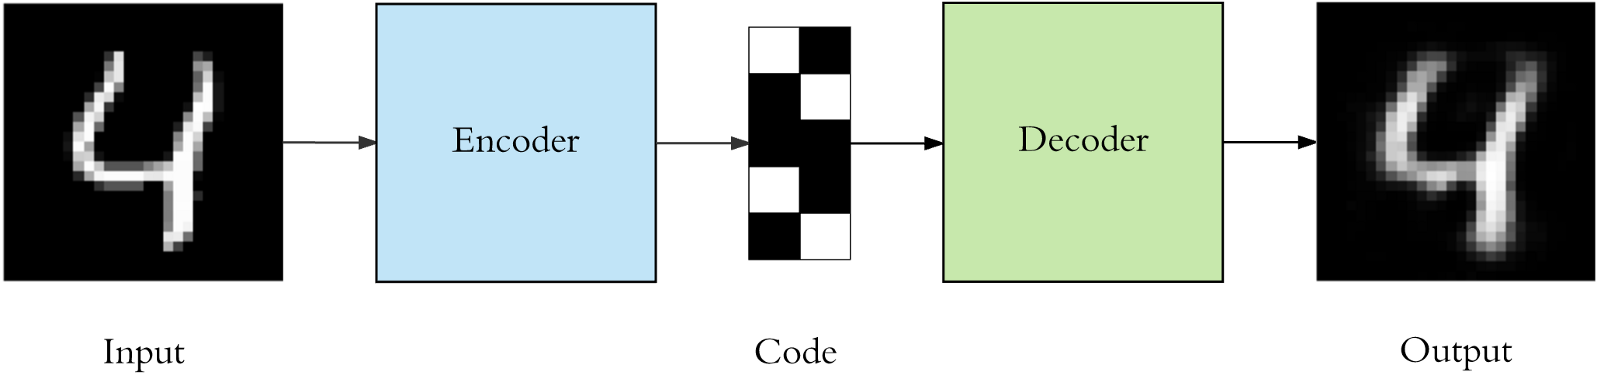
\includegraphics[width=8cm]{fig/cat-autoencoder.png}
	\end{center}
\end{frame}

\begin{frame}[c]{Goal Recognition using Raw Data}
	\begin{itemize}
		\item Once we learn the internal representation, we can recognize plans as sequences of images, but using symbolic goal recognition algorithms
	\end{itemize}
	\begin{center}
		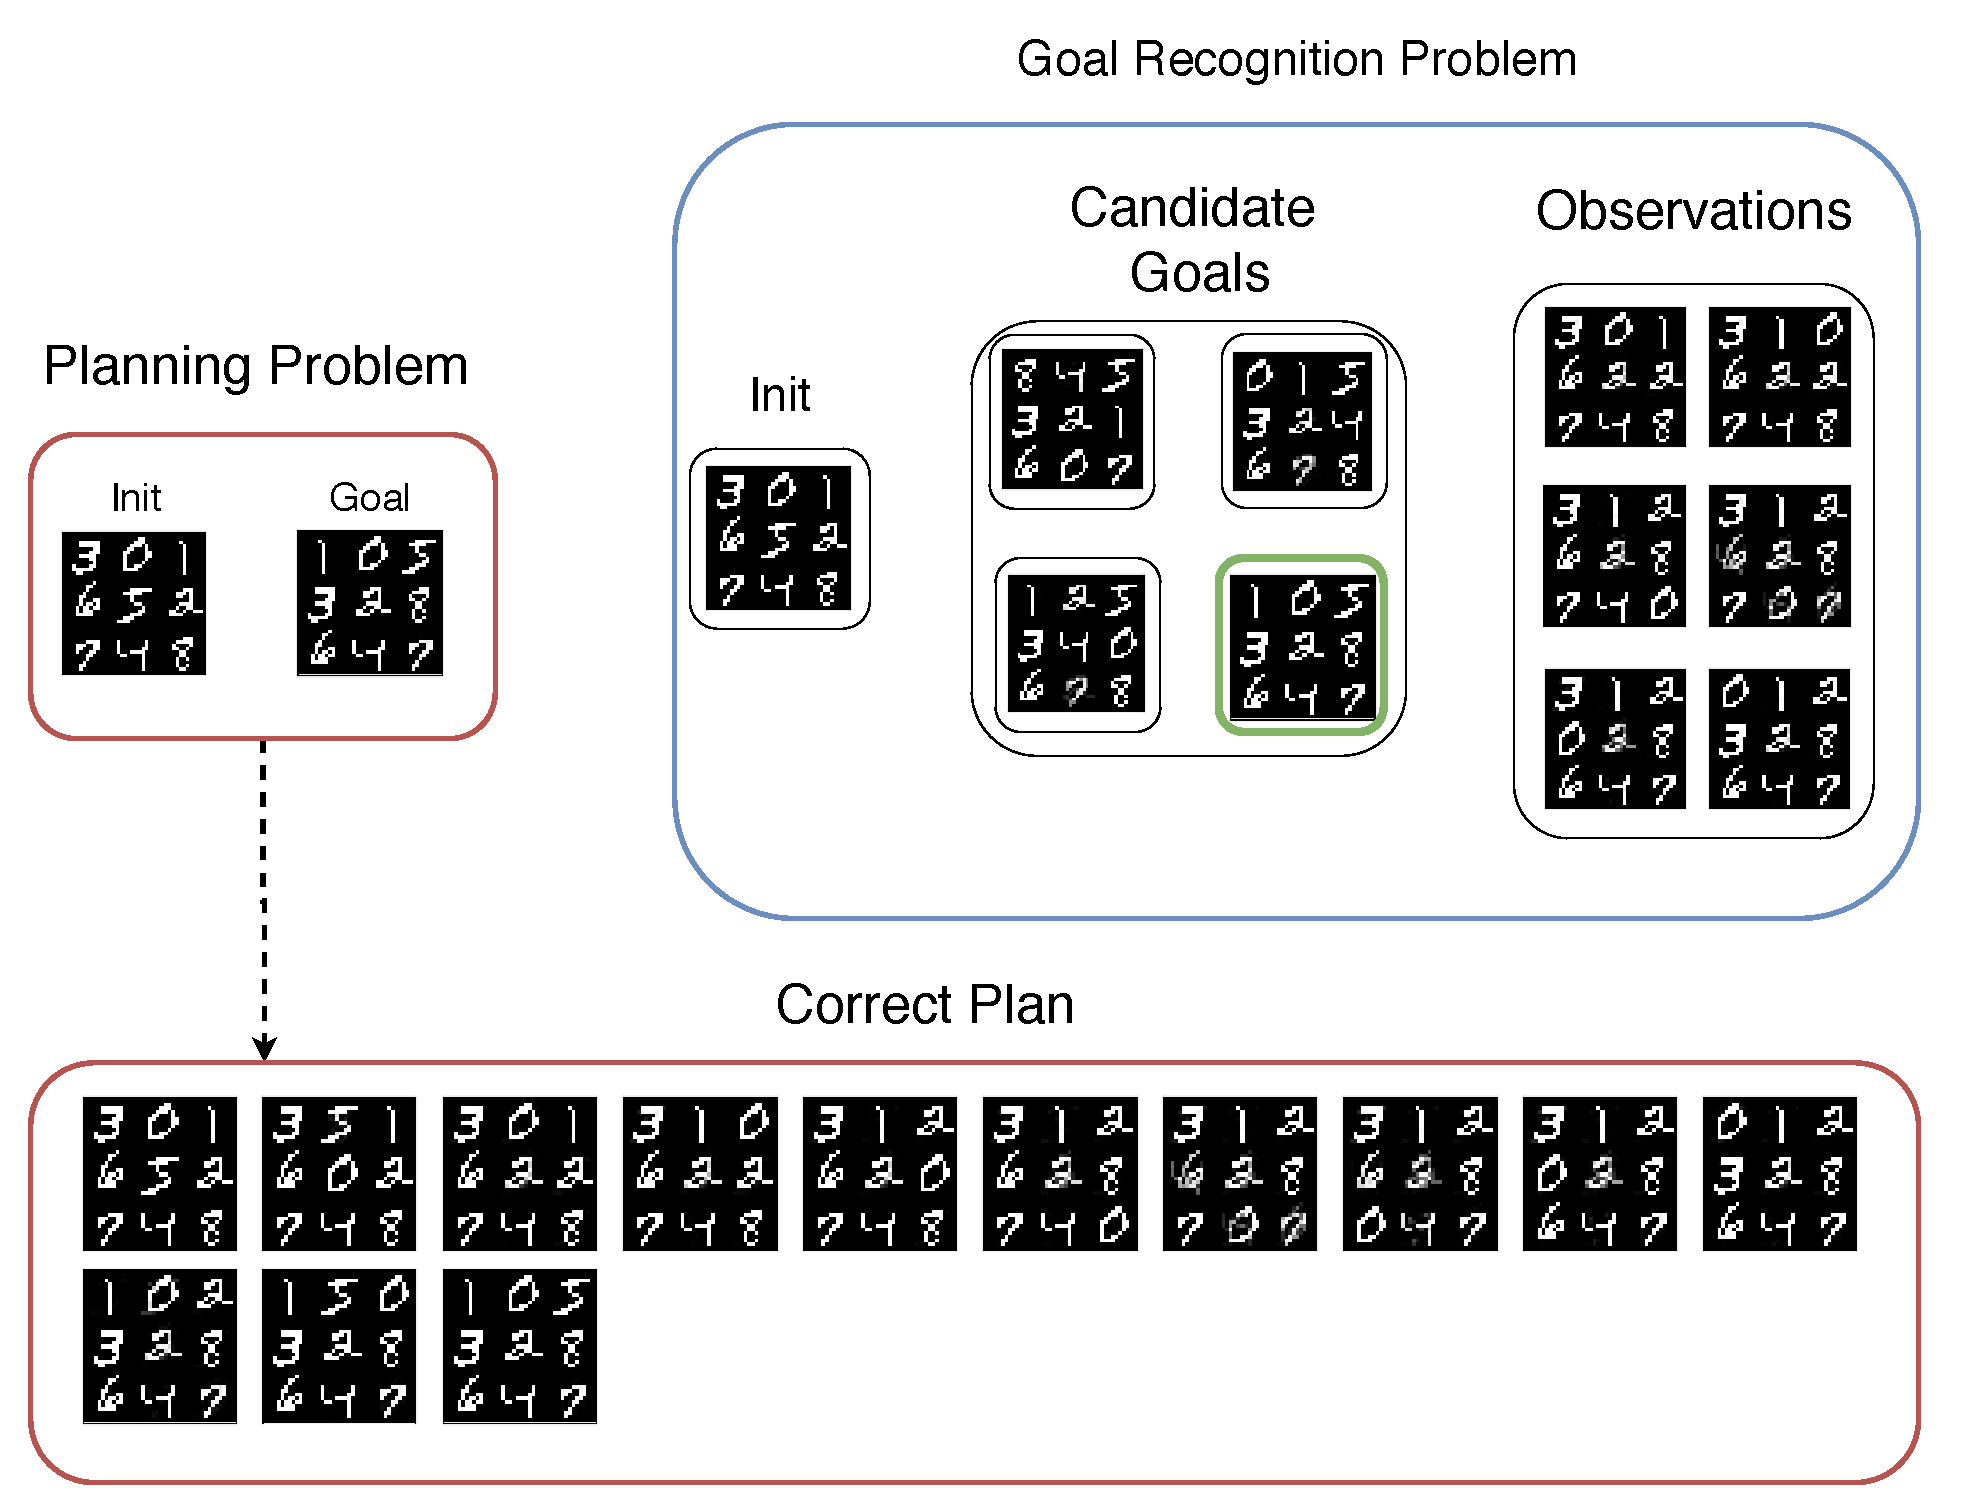
\includegraphics[width=8cm]{fig/lat_rec_problem.pdf}
	\end{center}
\end{frame}

\begin{frame}[c]{Goal Recognition in Latent Space}
	\begin{columns}
		\begin{column}{.35\textwidth}
			Key steps in the approach
			\small
			\begin{itemize}
				\item Train autoencoder using an image dataset (binary representation)
				\item Infer transition function from pairs of encoded images (states)
				\item Convert Goal Recognition problem to latent space using autoencoder
				\item Recognize goals using PRAP algorithms (ours)
			\end{itemize}
		\end{column}
		\begin{column}{.6\textwidth}
			\begin{center}
				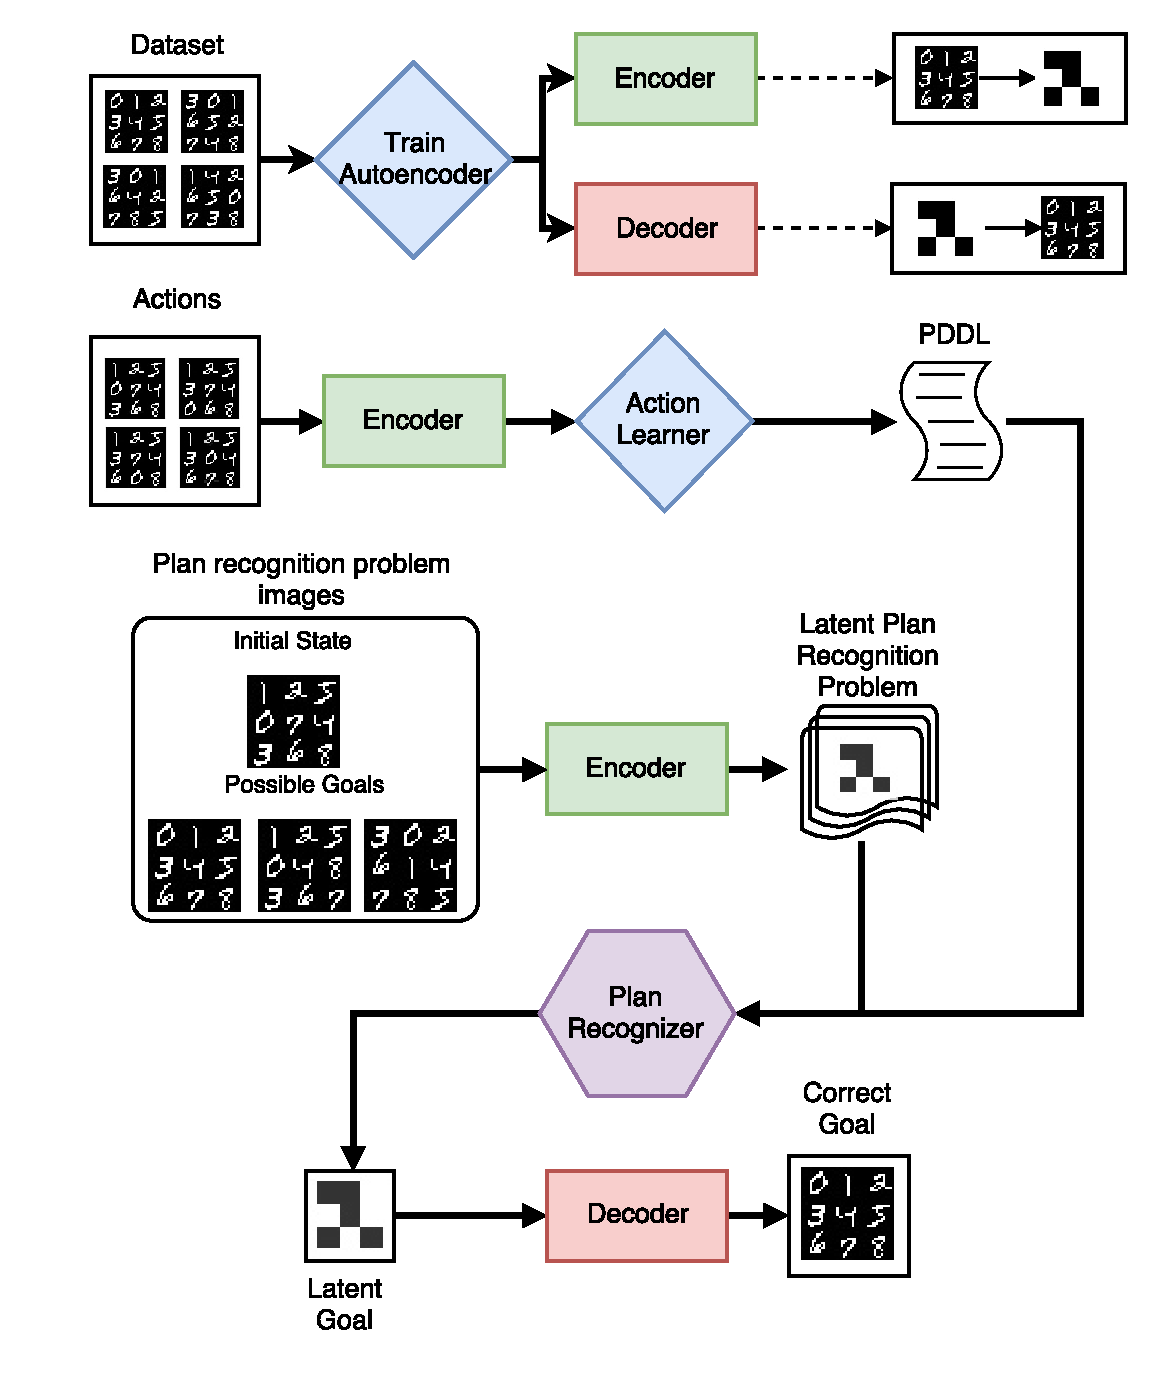
\includegraphics[width=.85\textwidth]{fig/IGR_Full.pdf}
			\end{center}
		\end{column}
	\end{columns}
\end{frame}

\begin{frame}[c]{How are we doing so far?}
	\begin{itemize}
		\item To Generate Symbolic Observations:
		\begin{itemize}
			\item ML to map raw data into a recognition algorithm {\Large \checkmark}
			\item ML algorithms to generate \textbf{symbolic observations} 
		\end{itemize}
		\item Obtain Domain Knowledge:
		\begin{itemize}
			\item Cope with expected noisy observations relaxing the domain model {\Large \checkmark}
			\item Learn PDDL representations from image data {\Large \color{red} \checkmark}
			\item Learn \textbf{Nominal Models} from raw data
		\end{itemize}
		\item To work on both problem simultaneously
		\begin{itemize}
			\item Hybrid engineering/learning of PDDL representations 
		\end{itemize}
	\end{itemize}
\end{frame}

\subsection{Goal Recognition Using Nominal Models}

\begin{frame}[c]
	\begin{center}
		\Large{Goal Recognition Using Nominal Models}
	\end{center}
\end{frame}

    \begin{frame}{Motivation}
       	\begin{itemize}
       		\item Existing goal recognition approaches \textbf{rely on complete models} with \textbf{known system dynamics};
			% Even recognition approaches that deal with incomplete domains assume that the transition function is given and well defined.
			
			\vspace{3mm}
			\item We \textbf{drop the assumption} that the transition function is given and well defined, using \textbf{Nominal (approximate) models}
		\end{itemize}
		\begin{figure}[]
		 	\centering
			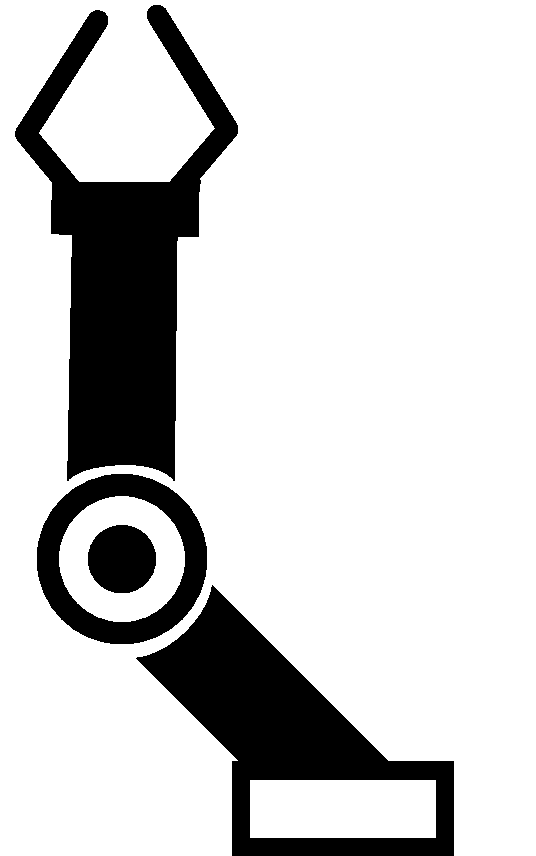
\includegraphics[width=0.25\linewidth]{fig/robotic-arm-0.pdf}
		 	
\includegraphics[width=0.25\linewidth]{fig/robotic-arm-1.pdf}
			\hspace{2mm}
			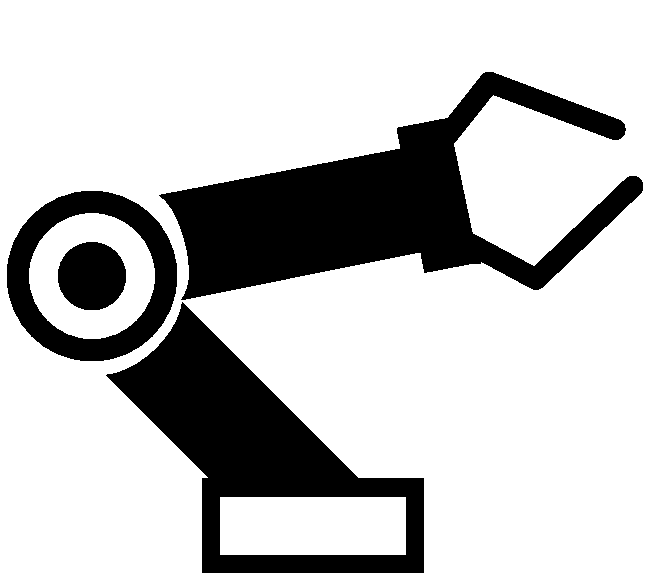
\includegraphics[width=0.3\linewidth]{fig/robotic-arm-2.pdf}
		\end{figure}
    \end{frame}	
	
		%     \begin{frame}{Introduction}
		%        	\begin{itemize}
		% 	\vspace{3mm}
		% 	\item We can learn \textbf{Nominal models} from observations on transitions of systems;
		% 		\begin{itemize}
		% 			\vspace{1.5mm}
		% 			\item We use \textbf{Deep Neural Networks} to obtain \textit{nominal models};
		% 			\vspace{1.5mm}
		% 			\item \textit{Nominal models} support \textbf{continuous} action and state spaces;
		% 		\end{itemize}
		%
		% 	\vspace{3mm}
		% 	\item We \textbf{adapt two goal recognition approaches} to cope with \textit{nominal models};
		% 	\begin{itemize}
		% 		\item Performing \textbf{offline and online} goal recognition.
		% 	\end{itemize}
		% \end{itemize}
		%     \end{frame}
	
	% Slides skipped from the original
	
    \begin{frame}[c]{Deep Neural Networks as Nominal Models}
		\begin{center}
			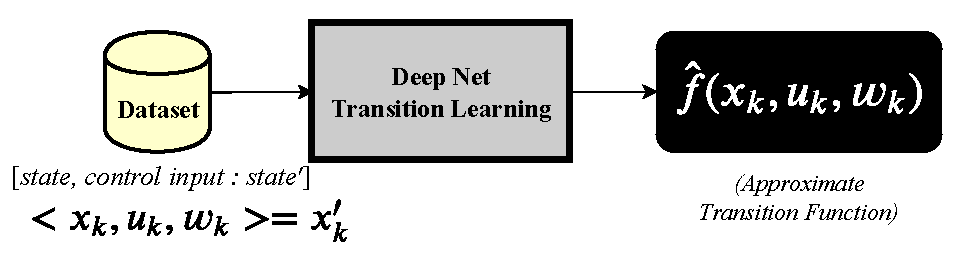
\includegraphics[width=0.95\linewidth]{fig/DNNs_as_NominalModels.pdf}
		\end{center}
		% \begin{figure}[]
% 		 	\centering
%
% 			\caption{DNNs as Nominal Models.}
% 		\end{figure}
		
			\begin{itemize}
				% \item To acquire \textbf{nominal models} we use a DNN developed by Say et al. (IJCAI, 2017)\footnote{\tiny \it Say et al., Nonlinear Hybrid Planning with Deep Net Learned Transition Models and Mixed-Integer Linear Programming. IJCAI, 2017.}.
				\item We acquire \textbf{nominal models} by training a DNN
				\item Trained DNN becomes the \textbf{transition function}
				\item \textit{Nominal models} support \textbf{continuous} action and state spaces;
			\end{itemize}		
    \end{frame}
	
    \begin{frame}[c]{Goal Recognition over Nominal Models}
		\begin{center}
			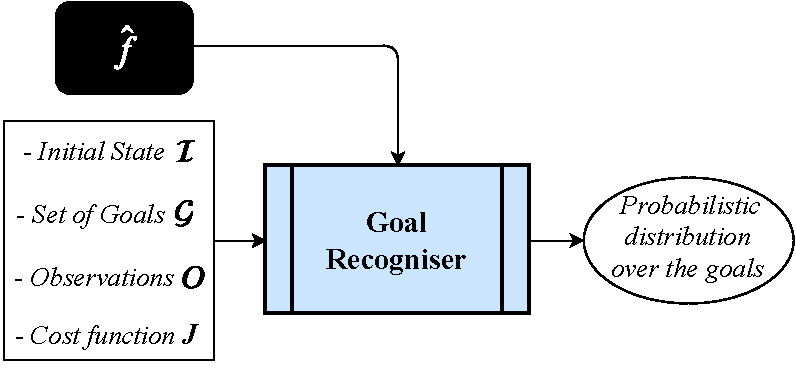
\includegraphics[width=0.85\linewidth]{fig/GR_ApproximatedModels-ProblemOverview.pdf}
		\end{center}
		
		\begin{itemize}
			\item We define the observations $O$ as \textbf{\emph{trajectory} of \emph{states}} induced by a policy
	$\pi$ that minimises $J$, and \textbf{achieve a hidden goal} $G^* \in \mathcal{G}$.
		\end{itemize}
    \end{frame}
	
    \begin{frame}{Probabilistic Goal Recognition over Nominal Models}
			We adopt the probabilistic interpretation of Ramírez and Geffner (2010)\footnote{\tiny \it Ramírez and Geffner, Probabilistic Plan Recognition using off-the-shelf Classical Planners. AAAI, 2011.}:
			\vspace{2mm}
			\begin{itemize}
				\item $P(G|O) = \alpha P(O|G) P(G)$
				\vspace{1mm}
				\begin{itemize}
					\item $P(G)$ is a \emph{prior} probability to a goal $G$;
					\vspace{1.5mm}
					\item $P(O|G)$ is the probability of observing $O$ when the goal is $G$;
					\vspace{1.5mm}
					\item $\alpha$ is a normalisation factor.
				\end{itemize}
			\end{itemize}
			\vspace{5mm}
			Here, since $P(G)$ is equal for every candidate goal, the question is: 
			\begin{itemize}
				\item \textbf{How do we compute $P(O|G)$}?
			\end{itemize}
    \end{frame}
	
    \begin{frame}{Goal Recognition as Nominal Mirroring: $\eta$\textsc{Mirroring}}
			We develop our first approach using the concept of \emph{Mirroring}\footnote{\tiny \it Vered et al., Online Goal Recognition through Mirroring: Humans and Agents. ACS, 2016.} to \textbf{compare two plans for each of the candidate goals in} $\mathcal{G}$:
			\vspace{2mm}
	       	\begin{itemize}
				\vspace{2mm}
	       		\item \textbf{Ideal-plan} ($\pi_G$): a plan computed from $\mathcal{I}$ to every goal $G$ in $\mathcal{G}$;
				\vspace{2mm}
				\item \textbf{$O$-plan} ($\pi_{O,G}$): a plan computed for every pair ${\cal I}$, $G$, which must visit every state in $O$. 
			\end{itemize}
    \end{frame}
	
    \begin{frame}{$\eta$\textsc{Mirroring}: \emph{matching-error} {\huge $\epsilon$}}
		We compare the \textbf{Ideal-plan} and the \textbf{$O$-plan} using the \emph{matching-error}\footnote{\tiny \it Kaminka et al., Plan Recognition in Continuous Domains. AAAI, 2018.} {\huge $\epsilon$}, i.e., the \textbf{Euclidean distance} between the trajectories.

		\begin{figure}[]
		 	\centering
		 	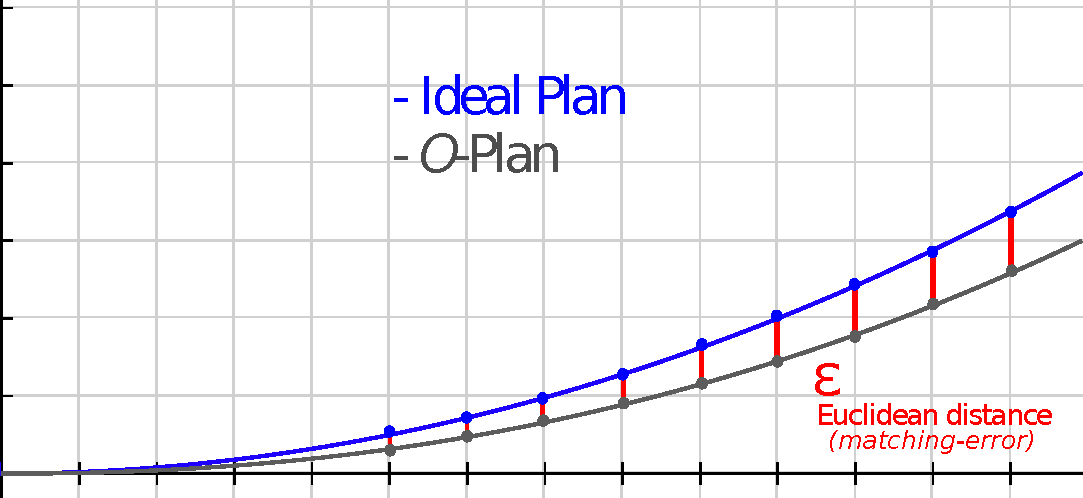
\includegraphics[width=0.85\linewidth]{fig/nominal_mirroring.pdf}
			\vspace{-2mm}
		\end{figure}
    \end{frame}

\begin{frame}[c]{How are we doing so far?}
	\begin{itemize}
		\item To Generate Symbolic Observations:
		\begin{itemize}
			\item ML to map raw data into recognition algorithm {\Large \checkmark}
			\item ML algorithms to generate \textbf{symbolic observations} 
		\end{itemize}
		\item Obtain Domain Knowledge:
		\begin{itemize}
			\item Cope with expected noisy observations relaxing the domain model {\Large \checkmark}
			\item Learn PDDL representations from image data {\Large \checkmark}
			\item Learn \textbf{Nominal Models} from raw data {\Large \color{red} \checkmark}
		\end{itemize}
		\item To work on both problem simultaneously
		\begin{itemize}
			\item Hybrid engineering/learning of PDDL representations 
		\end{itemize}
	\end{itemize}
\end{frame}

% \subsection{LSTM-based plan recognition}
%
% \begin{frame}[c]
% 	\begin{center}
% 		\Large{LSTM-based plan recognition}
% 	\end{center}
% \end{frame}
%
% \begin{frame}[c]{Placeholder slide}
%
% \end{frame}
%
% \begin{frame}[c]{How do we try to solve this?}
% 	\begin{itemize}
% 		\item To Generate Symbolic Observations:
% 		\begin{itemize}
% 			\item ML to map raw data into recognition algorithm {\Large \checkmark}
% 			\item ML algorithms to generate \textbf{symbolic observations}
% 		\end{itemize}
% 		\item Obtain Domain Knowledge:
% 		\begin{itemize}
% 			\item Cope with expected noisy observations relaxing the domain model {\Large \checkmark}
% 			\item Learn PDDL representations from image data {\Large \checkmark}
% 			\item Learn \textbf{Nominal Models} from raw data {\Large \color{red} \checkmark}
% 		\end{itemize}
% 		\item To work on both problem simultaneously
% 		\begin{itemize}
% 			\item Hybrid engineering/learning of PDDL representations
% 		\end{itemize}
% 	\end{itemize}
% \end{frame}

\subsection{Engineering GR Domains using ML}

\begin{frame}[c]
	\begin{center}
		\Large{Engineering GR Domains using ML}
	\end{center}
\end{frame}

% \begin{frame}[c]{Placeholder}
% 	 \includegraphics[width=.9\textwidth]{../placeholder2.pdf}
% \end{frame}
%
% \begin{frame}[c]{Placeholder}
% 	 \includegraphics[width=.9\textwidth]{../placeholder1.pdf}
% \end{frame}

\begin{frame}[c]{Machine Learning and Computer Vision}
	\begin{columns}
		\begin{column}{.6\textwidth}
			\begin{itemize}
				\item<1-> Machine Learning models are the unchallenged state of the art for computer vision: %\\ \onslide<2-> {~\color{red} Deal with it}
				\item<2-> Most computer vision datasets already contain \textbf{annotated semantic information} (and algorithms assume their existence):
				\begin{itemize}
					\item Labels for \textbf{objects} and \textbf{relations}
				\end{itemize}
				\item<2-> Why not use this semantic information to co-design GR domains around them?
			\end{itemize}
		\end{column}
		\begin{column}{.4\textwidth}
			\only<1>{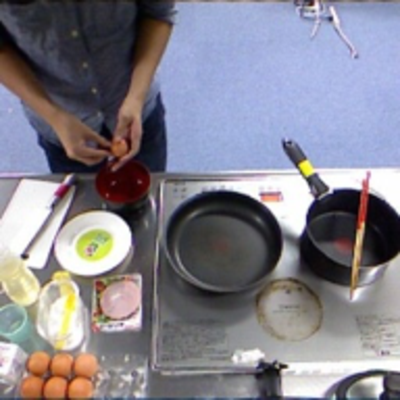
\includegraphics[width=\textwidth]{fig/computer-vision-eggs.pdf}}
			\only<2->{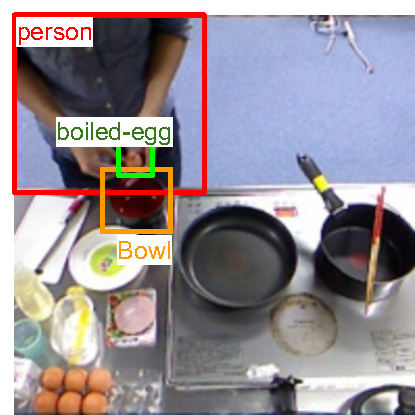
\includegraphics[width=\textwidth]{fig/computer-vision-annotated.pdf}
			Relations:\\
			\footnotesize
			\texttt{<{\color{red}person},{\color{black}holding},{\color{OliveGreen}boiled-egg}>}\\
			\texttt{<{\color{OliveGreen}boiled-egg},{\color{black}holding},{\color{orange}bowl}>}
			}
			
		\end{column}
	\end{columns}
\end{frame}

\begin{frame}[c]{Deriving PDDL from ML Algorithms}
	\begin{center}
		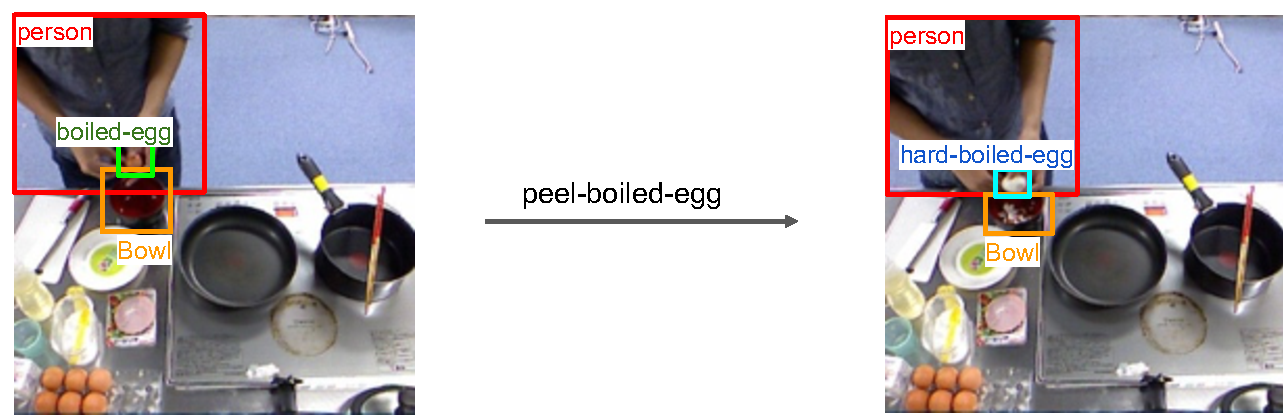
\includegraphics[width=.9\textwidth]{fig/computer-vision-transition1.pdf}
	\end{center}
	\begin{columns}
		\begin{column}{.4\textwidth}
			Relations:\\
			\footnotesize
			\texttt{<{\color{red}person},{\color{black}holding},{\color{OliveGreen}boiled-egg}>}\\
			\texttt{<{\color{OliveGreen}boiled-egg},{\color{black}holding},{\color{orange}bowl}>}
		\end{column}
		\begin{column}{.6\textwidth}
			\lstinputlisting[basicstyle=\fontsize{7}{7.7}\selectfont,language=LISP]{examples/kitchen-learned.pddl.txt}
		\end{column}
	\end{columns}
\end{frame}

\begin{frame}[c]{Generating Semantically-meaningful Observations with ML}
	\begin{center}
		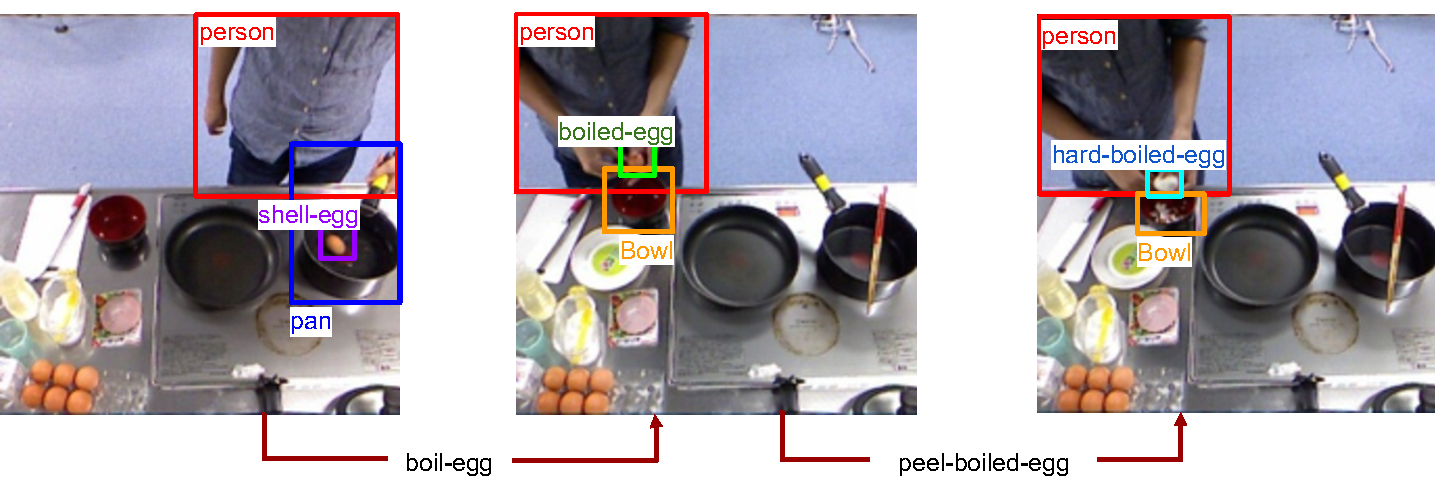
\includegraphics[width=\textwidth]{fig/computer-vision-transition-boiled-egg.pdf}
	\end{center}
	\begin{columns}
		\begin{column}{.3\linewidth}
			\tiny
			\texttt{<{\color{red}person},{\color{black}holding},{\color{purple}shell-egg}>}\\
			\texttt{<{\color{Magenta}shell-egg},{\color{black}in},{\color{blue}pan}>}\\
			\texttt{<{\color{red}person},{\color{black}holding},{\color{black}hashi}>}\\
			% \texttt{<{\color{black}hashi},{\color{black}moving},{\color{black}egg}>}
		\end{column}
		\begin{column}{.3\linewidth}
			\tiny
			\texttt{<{\color{red}person},{\color{black}holding},{\color{OliveGreen}boiled-egg}>}\\
			\texttt{<{\color{OliveGreen}boiled-egg},{\color{black}on},{\color{orange}bowl}>}
		\end{column}
		\begin{column}{.3\linewidth}
			\tiny
			\texttt{<{\color{red}person},{\color{black}holding},{\color{blue}hard-boiled-egg}>}\\
			\texttt{<{\color{OliveGreen}hard-boiled-egg},{\color{black}on},{\color{orange}bowl}>}
		\end{column}
	\end{columns}
\end{frame}

\begin{frame}[c]{How are we doing so far?}
	\begin{itemize}
		\item To Generate Symbolic Observations:
		\begin{itemize}
			\item ML to map raw data into recognition algorithm {\Large \checkmark}
			\item ML algorithms to generate \textbf{symbolic observations} {\Large \color{red} \checkmark}
		\end{itemize}
		\item Obtain Domain Knowledge:
		\begin{itemize}
			\item Cope with expected noisy observations relaxing the domain model {\Large \checkmark}
			\item Learn PDDL representations from image data {\Large \checkmark}
			\item Learn \textbf{Nominal Models} from raw data {\Large \checkmark}
		\end{itemize}
		\item To work on both problem simultaneously
		\begin{itemize}
			\item Hybrid engineering/learning of PDDL representations {\Large \color{red} \checkmark}
		\end{itemize}
	\end{itemize}
\end{frame}

% @@@@@@@@@@@@@@@@@@@@@@@@@@@@@@@@@@@@@@@@@@@@@@@@@@@@@@@@@@@@@@@

% \section{Goal Recognition as reasoning over Heuristics}
%
% \if\masterclass1
% 	\begin{frame}[c]\frametitle{Goal Recognition}
% 		Background on other PRAP approaches:
% 		\begin{itemize}
% 			\item Ramirez and Geffner
% 			\item Martin
% 			\item Sohrabi
% 		\end{itemize}
% 	\end{frame}
% 	\begin{frame}[c]\frametitle{Previous Work: Ramirez and Geffner}
% 		\if\masterclass1
% 		\todo{Move this to the background}
% 		\fi
% 		\begin{itemize}
% 			\item First approaches to goal recognition: Plan Recognition as Planning (PRAP)
% 			\item Probabilistic model aims to compute $P(G \mid O)$
% 			\item Following Bayes Rule $P(G \mid O) = \alpha P(O \mid G) P(G)$
% 			\item Given $P(G)$ as a prior, key bottleneck is computing $P(O \mid G)$
% 			\begin{itemize}
% 				\item In their work $P(O \mid G)$ is computed in terms of a cost difference $c(G,O) - c(G,\bar{O})$
% 				\item Computational cost is \textbf{two planner calls per goal hypothesis}
% 				\item For online recognition: two planner calls per goal hypothesis \textbf{per observation}
% 			\end{itemize}
% 			\item Some conclusions challenged for path planning domains\\ (Masters and Sardina 2017)
% 		\end{itemize}
% 	\end{frame}
% \fi
%
%     \begin{frame}{Motivation}
%        	\begin{itemize}
% 			\item In this work, we use a \textbf{planning domain definition} to represent agent behavior and environment properties;
% 			\item Previous approaches involve multiple calls to a modified planner.
% 			\item Our main contribution is twofold:
% 				\begin{itemize}
% 					\item We \textbf{obviate the need to execute a planner multiple times} for recognizing goals; and
% 					\item We develop novel goal recognition heuristics that \textbf{use planning landmarks}.
% 				 \end{itemize}
% 			% \item We evaluate our approaches against the fastest and most accurate approach of Ramírez and Geffner ({\footnotesize Plan Recognition as Planning. IJCAI, 2009}) over \textbf{15 planning domains};
% 			\item We show that our approaches are \textbf{more accurate} and \textbf{orders of magnitude faster} than Ramírez and Geffner's approach.
% 		\end{itemize}
%     \end{frame}
%
% \if\masterclass1
% 	\begin{frame}[c]\frametitle{Planning Heuristics}
% 		Material about the planning heuristics
% 	\end{frame}
%
%     \begin{frame}{Background: Planning and Landmarks}
% 		\begin{definition} [\textbf{Planning}]
% 			\textit{A planning instance is represented by a triple $\Pi = \langle \Xi, \mathcal{I}, G\rangle$, in which:
% 			\begin{itemize}
% 				\item $\Xi$ $=$ $\langle$$\Sigma$, $\mathcal{A}$$\rangle$ is the \textbf{domain definition}, and consists of a finite set of \textbf{facts} $\Sigma$ and a finite set of \textbf{actions} $\mathcal{A}$ (action costs $=$ 1);
% 				\item $\mathcal{I}$ and $G$ represent the \textbf{planning problem}, in which $\mathcal{I}$ $\subseteq$ $\Sigma$ is the \textbf{initial state}, and $G$ $\subseteq$ $\Sigma$ is the \textbf{goal state}.
% 			\end{itemize}}
% 		\end{definition}
% 		\begin{definition}[\textbf{Landmarks}]
% 			\textit{Given a planning instance $\Pi = \langle \Xi, \mathcal{I}, G\rangle$, a \textbf{fact} (or \textbf{action}) $L$ is a landmark in $\Pi$ iff $L$ 	must be \textbf{satisfied} (or \textbf{executed}) at some point along all valid plans that achieve $G$ from $\mathcal{I}$.}
% 		\end{definition}
% 		\begin{itemize}
% 			\item To extract landmarks and their ordering, we use an algorithm developed by Hoffman \emph{et al.} {\footnotesize (Ordered Landmarks in Planning. JAIR, 2004)}.
% 		\end{itemize}
%     \end{frame}
% \fi
%
% %---------------------------------------------------------------------------------
%
%     \begin{frame}{Computing Achieved Landmarks}
% 		\if\masterclass1
% 		\todo{Change this example to the one from Ramirez}
% 		\fi
% 		\begin{center}
% 		    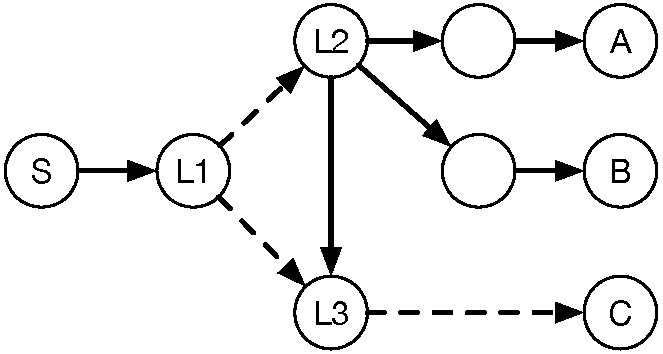
\includegraphics[width=.4\textwidth]{example.pdf}
% 		\end{center}
%
%        	\begin{itemize}
%        		\item Our heuristics require identifying which fact landmarks have been achieved during the observed plan execution for every candidate goal $G \in \mathcal{G}$;
%             \item For every candidate goal $G \in \mathcal{G}$:
%             	\begin{itemize}
%                 	\item Extract \emph{ordered} landmarks for $G$;
%                     \item Use achieved landmarks of $G$ in preconditions and effects of every observed action $o \in O$;
%                    \item Under partial observability, we deal with missing actions by inferring that predecessors of observed landmarks must have been achieved;
%                 \end{itemize}
% 		\end{itemize}
% % 		\begin{figure}[here]
% % 			\centering
% % 			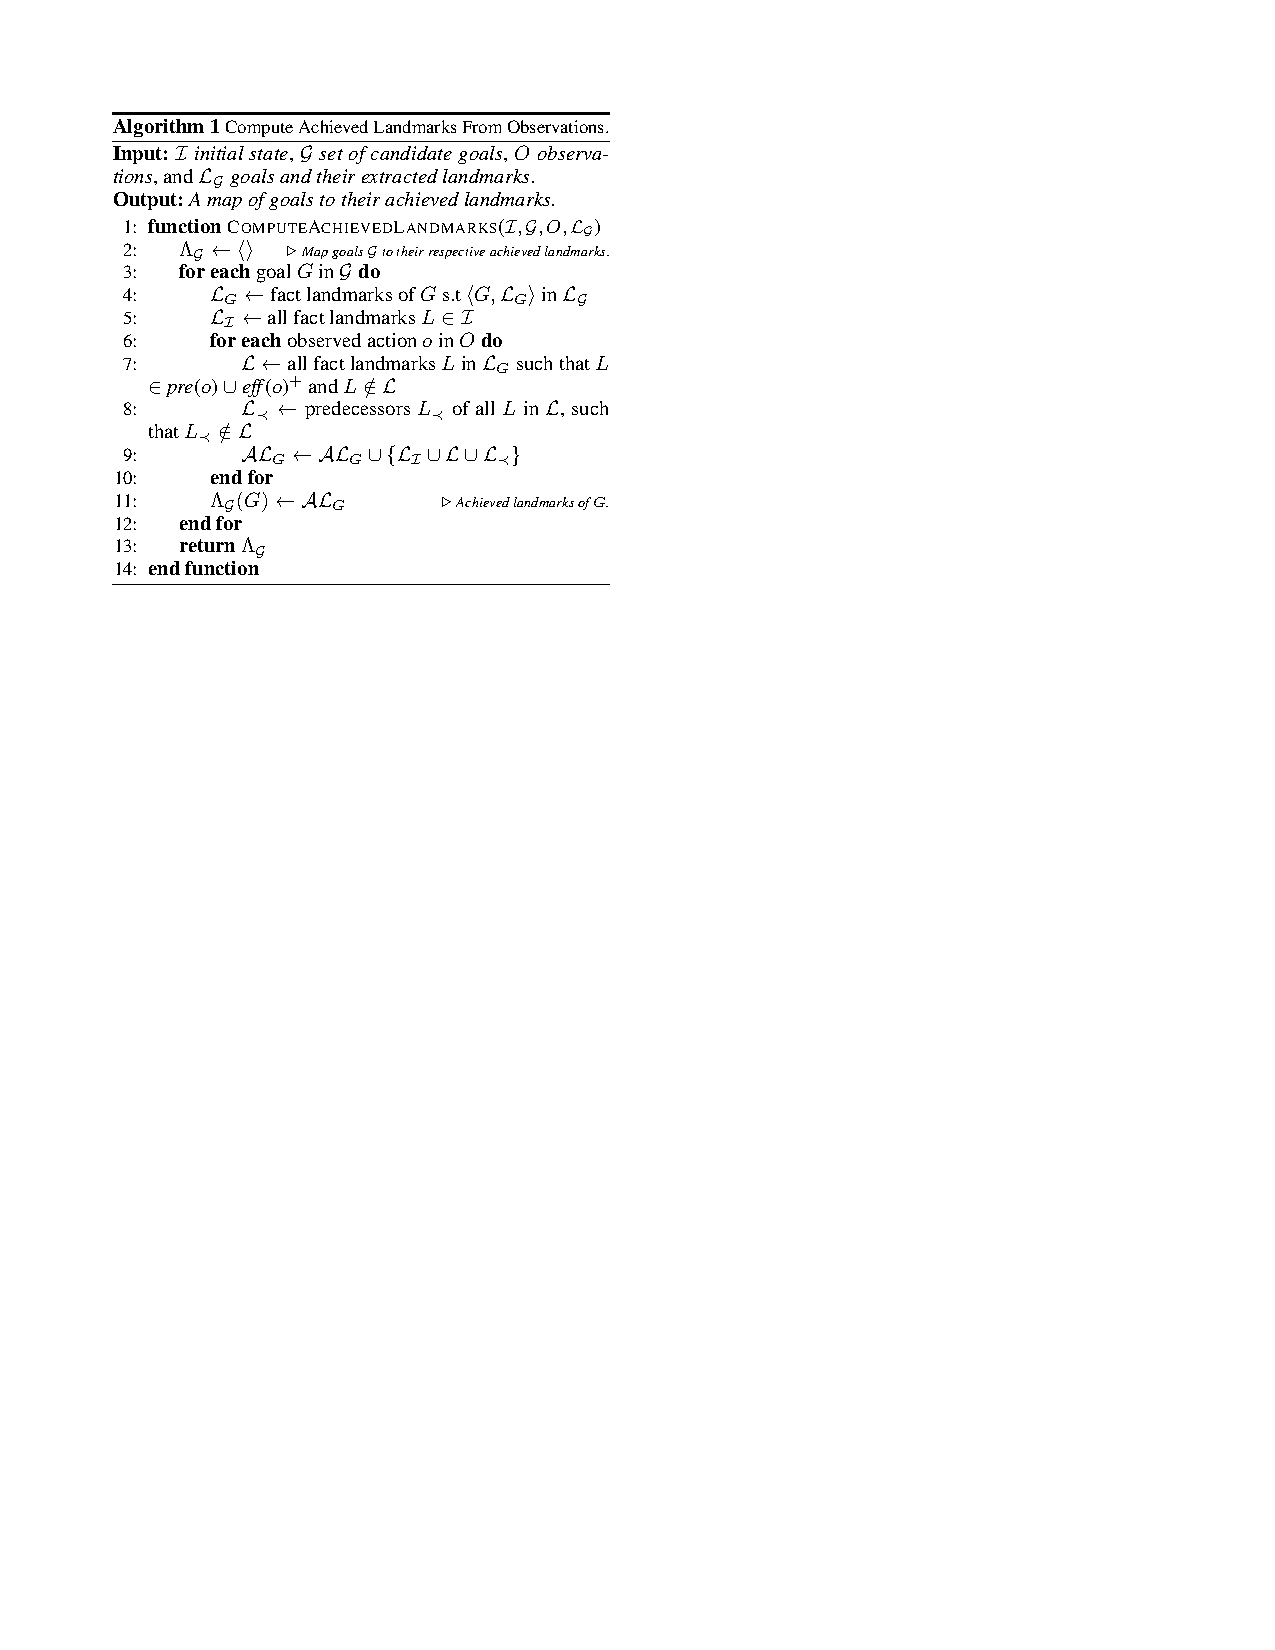
\includegraphics[width=0.65\linewidth]{algo1-computing_achieved_landmarks.pdf}
% % 		\end{figure}
%     \end{frame}
%
% %---------------------------------------------------------------------------------
%
%     \begin{frame}{Landmark-Based Goal Completion Heuristic}
%        	\begin{itemize}
%        		\item Goal Completion $h_{gc}$ aggregates the percentage of completion of each sub-goal into an overall percentage of completion for all facts of a candidate goal;
% 		\end{itemize}
%
% 		\begin{equation}
% 			h_{gc}(G, \mathcal{AL}_{G}, \mathcal{L}_{G}) = \left(\frac{\sum_{g \in G} \frac{|\mathcal{AL}_{g} \in \mathcal{AL}_{G} |}{|\mathcal{L}_{g} \in \mathcal{L}_{G}|}}{ |G| }\right)
% 		\end{equation}
% 		where:
% 		\begin{itemize}
% 			\item $\mathcal{AL}_{G}$ achieved landmarks for goals in $G$
% 			\item $\mathcal{L}_{G}$ all landmarks for goals in $G$
% 		\end{itemize}
%     \end{frame}
%
% % @@@@@@@@@@@@@@@@@@@@@@@@@@@@@@@@@@@@@@@@@@@@@@@@@@@@@@@@@@@@@@@
%
% \if\masterclass1
%     \begin{frame}{Landmark-Based Goal Completion Heuristic: Algorithm}
% 		\begin{itemize}
% 			\item Our approach allows the use of a threshold $\theta$, giving us \textbf{flexibility to avoid eliminating candidate goals} whose the percentage of goal completion are close to the highest completion value;
% 		\end{itemize}
%
% 		\begin{figure}[here]
% 			\centering
% 			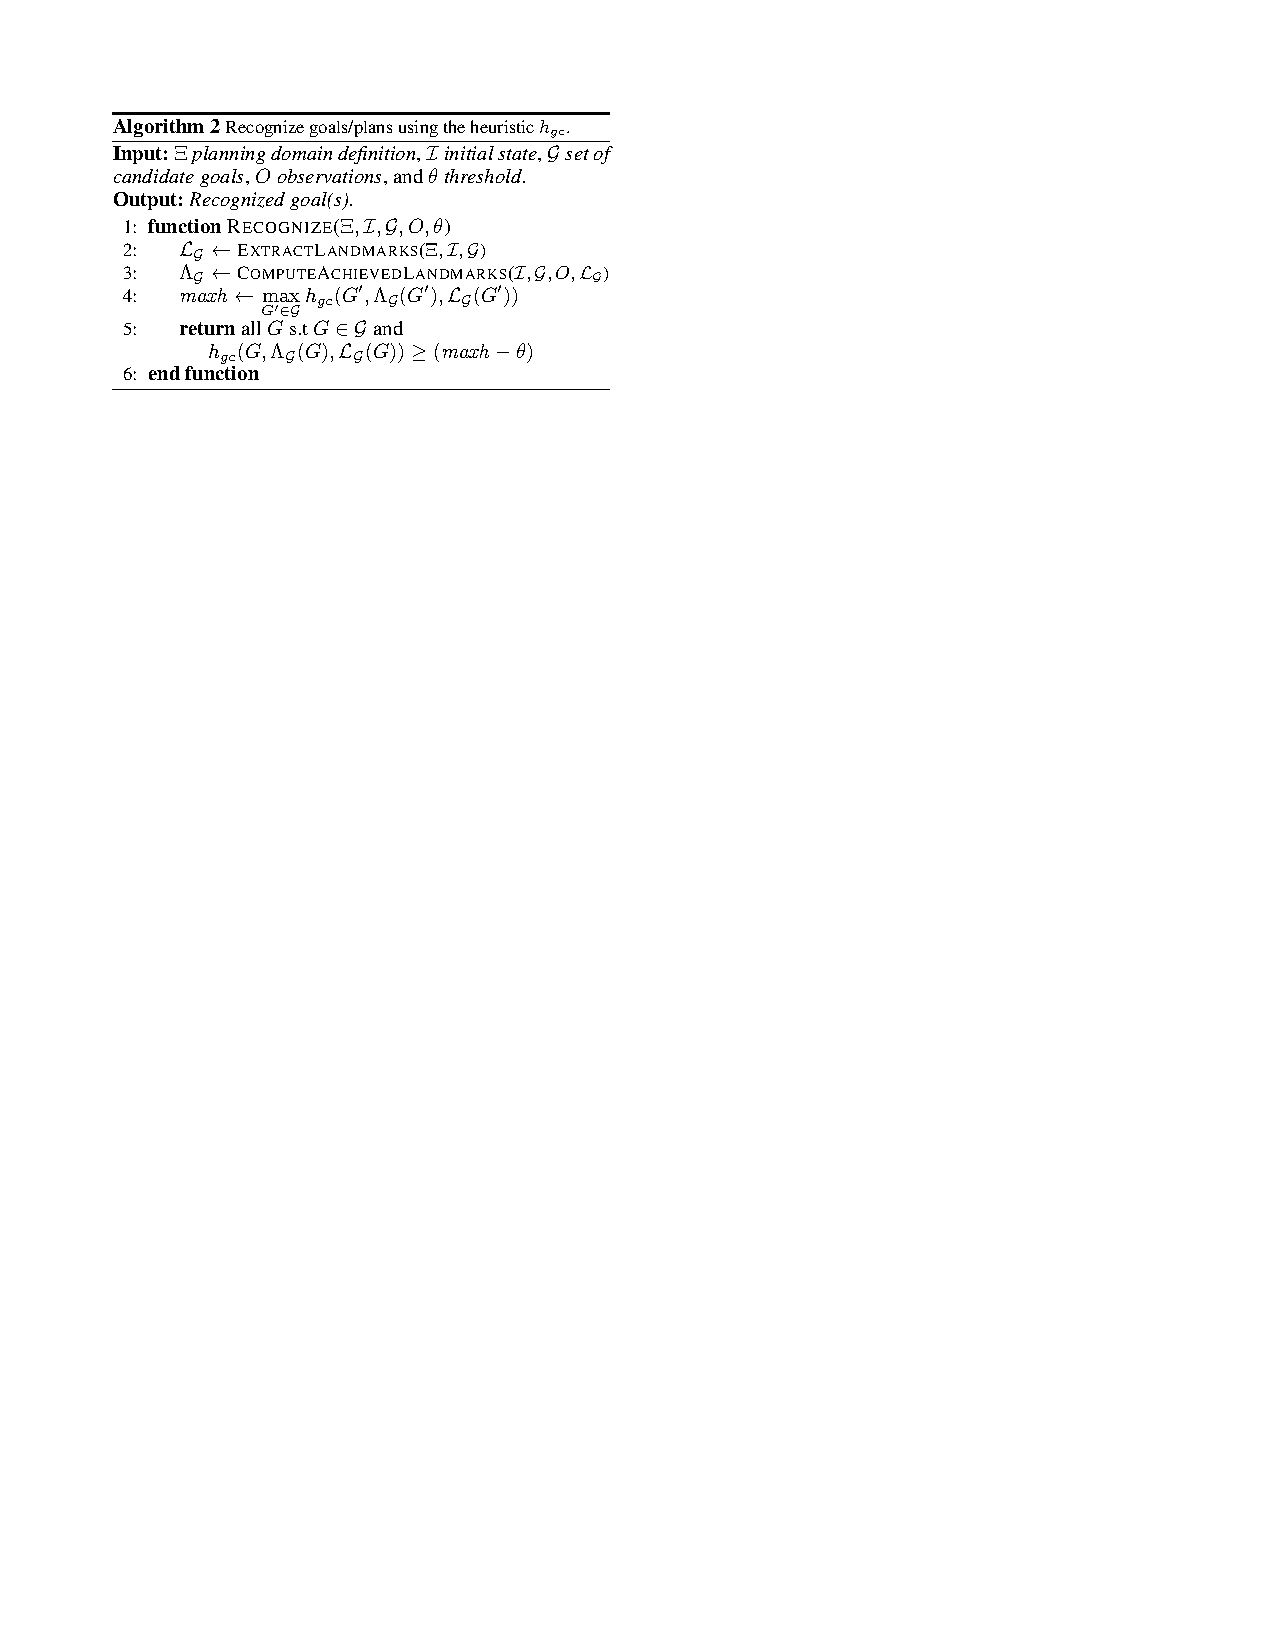
\includegraphics[width=0.8\linewidth]{algo2-heuristic_goalcompletion.pdf}
% 		\end{figure}
% 	\end{frame}
% \fi
%
% %---------------------------------------------------------------------------------
%
%     \begin{frame}{Landmark-Based Uniqueness Heuristic (1 of 2)}
%        	\begin{itemize}
%        		\item Our second heuristic computes \textbf{landmark uniqueness}: \\inverse frequency of a landmark within landmarks for candidate goals:%, \emph{i.e.}, how unique (and thus informative) each landmark is among all landmarks;
% 		\end{itemize}
%
% 		\begin{equation}
% 			L_{\mathit{Uniq}}(L, \mathcal{L}_{\mathcal{G}}) = \left(\frac{1}{\displaystyle\sum_{\mathcal{L} \in \mathcal{L_G}} |\{L |L \in \mathcal{L}\}|}\right)
% 		\end{equation}
%
% 		\begin{center}
% 		    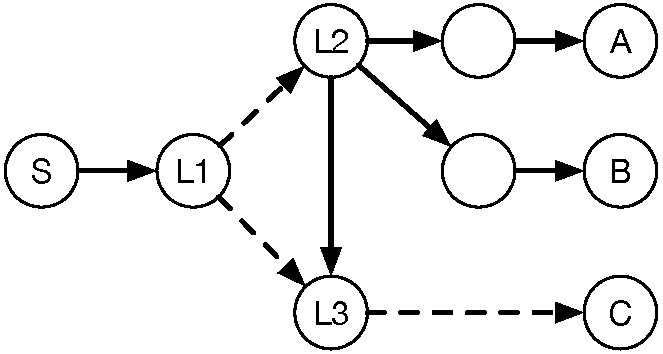
\includegraphics[width=.4\textwidth]{example.pdf}
% 			\quad
% 			\begin{minipage}{.4\textwidth}
% 				\vspace{-6em}
% 			  $L_{\mathit{Uniq}}(L2)=1/2$ \\
% 			  $L_{\mathit{Uniq}}(L1)=1/3$ \\
% 			  $L_{\mathit{Uniq}}(L3)=1$
% 			\end{minipage}
% 		\end{center}
%     \end{frame}
%
% % @@@@@@@@@@@@@@@@@@@@@@@@@@@@@@@@@@@@@@@@@@@@@@@@@@@@@@@@@@@@@@@
%
% 	\begin{frame}{Landmark-Based Uniqueness Heuristic (2 of 2)}
%
% 		\begin{itemize}
% 			\item Our second heuristic, called $h_{uniq}$, estimates the goal completion of a candidate goal $G$ by calculating the ratio between the sum of the uniqueness value of the achieved landmarks of $G$ and the sum of the uniqueness value of all landmarks of $G$;
% 		\end{itemize}
%
% 		\begin{equation}
% 		h_{\mathit{uniq}}(G, \mathcal{AL}_{G}, \mathcal{L}_{G}, \Upsilon_{uv}) = \left(
% 		\frac
% 		{\displaystyle\sum_{\mathcal{A}_{L} \in \mathcal{AL}_{G}}\Upsilon_{uv}(\mathcal{A}_{L})}
% 		{\displaystyle\sum_{L \in \mathcal{L}_{G}}\Upsilon_{uv}(L)}\right)
% 		\end{equation}
%
% 		where:
% 		\begin{itemize}
% 			\item $\Upsilon_{uv}$ is a table of uniqueness values
% 			\item $\mathcal{AL}_{G}$ achieved landmarks for goals in $G$
% 			\item $\mathcal{L}_{G}$ all landmarks for goals in $G$
% 		\end{itemize}
%
% 	\end{frame}
%
% % @@@@@@@@@@@@@@@@@@@@@@@@@@@@@@@@@@@@@@@@@@@@@@@@@@@@@@@@@@@@@@@
%
% \if\masterclass1
%     \begin{frame}{Landmark-Based Uniqueness Heuristic: Algorithm}
%        	\begin{itemize}
%        		\item Our second heuristic is called $h_{uniq}$;
% 		\end{itemize}
%
% 		\begin{figure}[here]
% 			\centering
% 			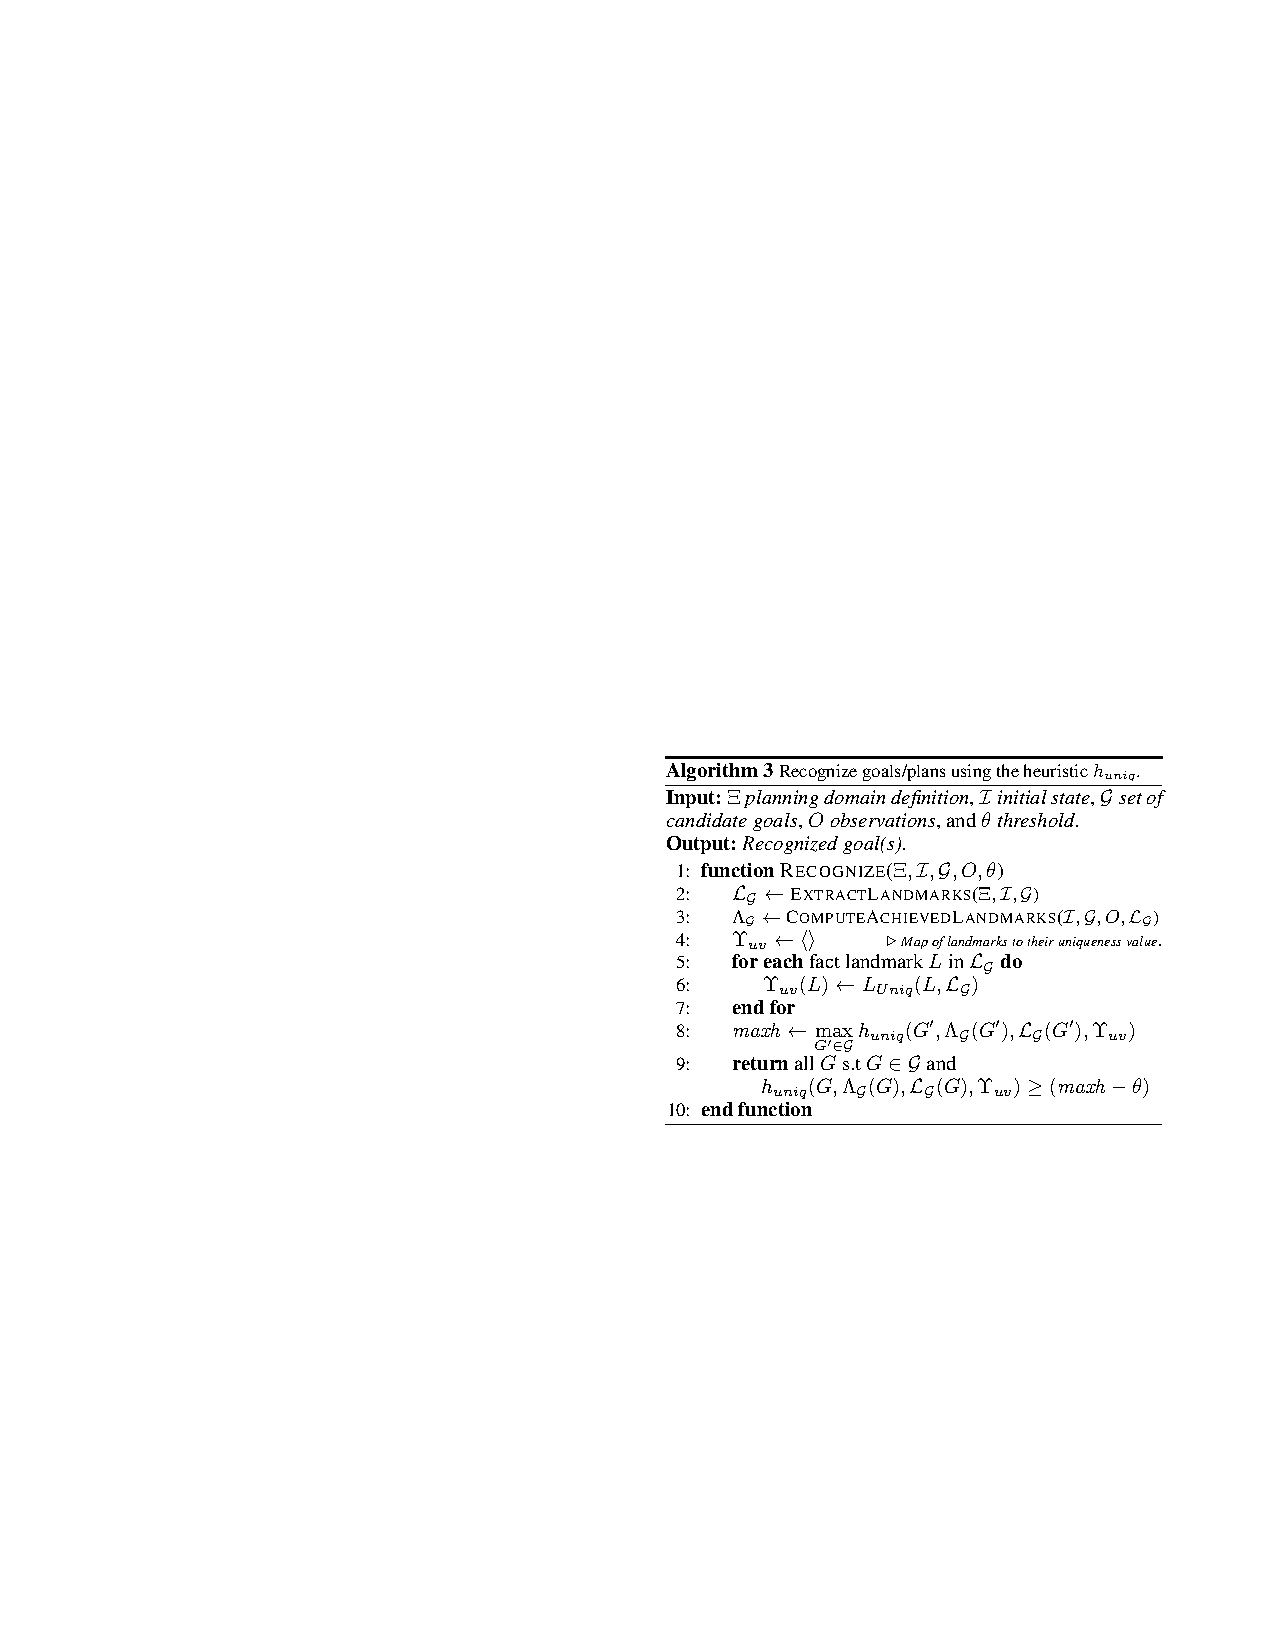
\includegraphics[width=0.75\linewidth]{algo3-heuristic_uniqueness.pdf}
% 		\end{figure}
%     \end{frame}
% \fi
% %---------------------------------------------------------------------------------
%
% % \if\masterclass1
%     \begin{frame}{Example (1 of 4)}
% 		\begin{figure}[here]
% 			\centering
% 			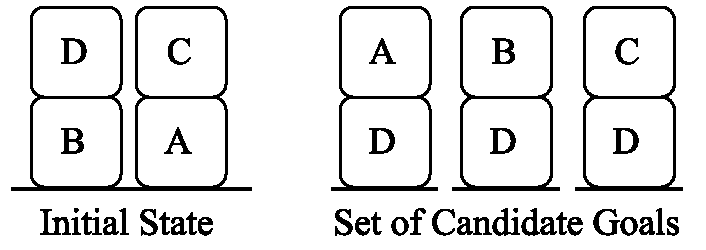
\includegraphics[width=0.75\linewidth]{example-blocksworld.pdf}
% 		\end{figure}
%        	\begin{itemize}
%        		\item Observations:
% 				\begin{itemize}
% 					\item \texttt{(unstack D B)}; and
% 					\item \texttt{(unstack C A)}.
% 				\end{itemize}
% 			\item The real goal is: \texttt{(and (ontable D) (on C D) (clear C))}
% 		\end{itemize}
%     \end{frame}
%
%     \begin{frame}{Example (2 of 4)}
% 		\textbf{Achieved Landmarks in Observations:}
%        	\begin{itemize}
%        		\item \texttt{(and (ontable D) (clear A) (on A D)), 5 out of 8}:
% 				\begin{itemize}
% 					\item {\scriptsize \texttt{[(clear A)]}, \texttt{[(clear A) (ontable A) (handempty)]},
% 					\\ \texttt{[(on C A) (clear C) (handempty)]}, \texttt{[(holding D)]},
% 					\\ \texttt{[(clear D) (on D B) (handempty)]}}
% 				\end{itemize}
% 			\item \texttt{(and (ontable D) (clear B) (on B D)), 4 out of 7}:
% 				\begin{itemize}
% 					\item {\scriptsize \texttt{[(clear B)]}, \texttt{[(ontable B) (handempty)]},
% 					\\ \texttt{[(on D B) (clear D) (handempty)]}, \texttt{[(holding D)]}}
% 				\end{itemize}
% 			\item \texttt{(and (ontable D) (clear C) (on C D)), 5 out of 7}:
% 				\begin{itemize}
% 					\item {\scriptsize \texttt{[(clear C)]}, \texttt{[(clear C) (on C A) (handempty)]}, \texttt{[(clear D) (holding C)]}
% 					\\ \texttt{[(clear D) (on D B) (handempty)]}, \texttt{[(holding D)]}}
% 				\end{itemize}
% 		\end{itemize}
%     \end{frame}
%
%     \begin{frame}{Example (3 of 4) - $h_{gc}$}
% 		\textbf{Landmark-Based Goal Completion Heuristic}
% 		% TODO break this down in more detail
%        	\begin{itemize}
%        		\item \texttt{(and (ontable D) (clear A) (on A D))}:%, 5 out of 8:
% 				\begin{itemize}
% 					\item Goal Completion: 0.7222
% 				\end{itemize}
% 			\item \texttt{(and (ontable D) (clear B) (on B D))}:%, 4 out of 7:
% 				\begin{itemize}
% 					\item Goal Completion: 0.6666
% 				\end{itemize}
% 			\item \texttt{(and (ontable D) (clear C) (on C D))}:%, 5 out of 7:
% 				\begin{itemize}
% 					\item \textbf{Goal Completion: 0.7777 (highest estimated value)}
% 				\end{itemize}
% 		\end{itemize}
%     \end{frame}
%
%     \begin{frame}{Example (4 of 4) - $h_{uniq}$}
% 		\textbf{Landmark-Based Uniqueness Heuristic}
%        	\begin{itemize}
%        		\item \texttt{(and (ontable D) (clear A) (on A D))}, Total$_{Uniq}$ = 5.5:
% 				\begin{itemize}
% 					\item {\scriptsize \texttt{[(clear A)] = 1}, \texttt{[(clear A) (ontable A) (handempty)] = 1},
% 					\\ \texttt{[(on C A) (clear C) (handempty)] = 0.5}, \texttt{[(holding D)] = 0.3333},
% 					\\ \texttt{[(clear D) (on D B) (handempty)] = 0.3333}}
% 					\item $h_{uniq}$ = 3.1666 / 5.5 = 0.5757
% 				\end{itemize}
% 			\item \texttt{(and (ontable D) (clear B) (on B D))}, Total$_{Uniq}$ = 5:
% 				\begin{itemize}
% 					\item {\scriptsize \texttt{[(clear B)] = 1}, \texttt{[(ontable B) (handempty)] = 1},
% 					\\ \texttt{[(on D B) (clear D) (handempty)] = 0.3333}, \texttt{[(holding D)] = 0.3333}}
% 					\item $h_{uniq}$ = 2.6666 / 5 = 0.5333
% 				\end{itemize}
% 			\item \texttt{(and (ontable D) (clear C) (on C D))}, Total$_{Uniq}$ = 4.5:
% 				\begin{itemize}
% 					\item {\scriptsize \texttt{[(clear C)] = 1}, \texttt{[(clear C) (on C A) (handempty)] = 0.5},
% 					\\ \texttt{[(clear D) (holding C)] = 1}, \texttt{[(holding D)] = 0.3333}
% 					\\ \texttt{[(clear D) (on D B) (handempty)] = 0.3333}}
% 					\item $h_{uniq}$ = 3.1666 / 4.5 = 0.71
% 				\end{itemize}
% 		\end{itemize}
%
% 		\textbf{Recognized} {\footnotesize \texttt{(and (ontable D) (clear C) (on C D))}} \textbf{with: }
% 		\\ $h_{uniq} = 0.71$
%     \end{frame}
%
% % % \if\masterclass1
% % \fi
% %---------------------------------------------------------------------------------
%
%     \begin{frame}{Experiments and Evaluation}
%        	\begin{itemize}
%        		\item We evaluate our heuristics over datasets with 15 planning domains \\(6 of these domains from original Ramírez and Geffner paper):
% 			\begin{itemize}
% 				\item {\footnotesize \textsc{Blocks-World, Campus, Depots, Driver-Log, Dock-Worker-Robots, Easy-IPC-Grid, Ferry, Intrusion-Detection, Kitchen, Logistics, Miconic, Rovers, Satellite, Sokoban, and Zeno-Travel}};
% 			\end{itemize}
% 			\item These datasets contain hundreds of goal recognition problems, varying the observability (10\%, 30\%, 50\%, 70\%, and 100\%);
% 			\item We compared our heuristics against the original approach of Ramírez and Geffner ({\footnotesize Plan Recognition as Planning. IJCAI, 2009}), which is their fastest and most accurate approach;
% 		\end{itemize}
%     \end{frame}
%
% % @@@@@@@@@@@@@@@@@@@@@@@@@@@@@@@@@@@@@@@@@@@@@@@@@@@@@@@@@@@@@@@
%
%     \begin{frame}{Experiments and Evaluation - ROC Space (1 of 2)}
%        	\begin{itemize}
%        		\item Results of our heuristics use threshold $\theta = $ 20\%;
% 			\item We compare Ramírez and Geffner's approach over ROC space,\\
% 			which shows the trade-off between TPR and FPR;
% 			\item We aggregate multiple domains and plot these goal recognition results in ROC space.
% 		\end{itemize}
% 	\end{frame}
%
% % @@@@@@@@@@@@@@@@@@@@@@@@@@@@@@@@@@@@@@@@@@@@@@@@@@@@@@@@@@@@@@@
%
% \begin{frame}{Experiments and Evaluation - ROC Space (2 of 2)}
% 	\begin{figure}[here]
% 		\centering
% 		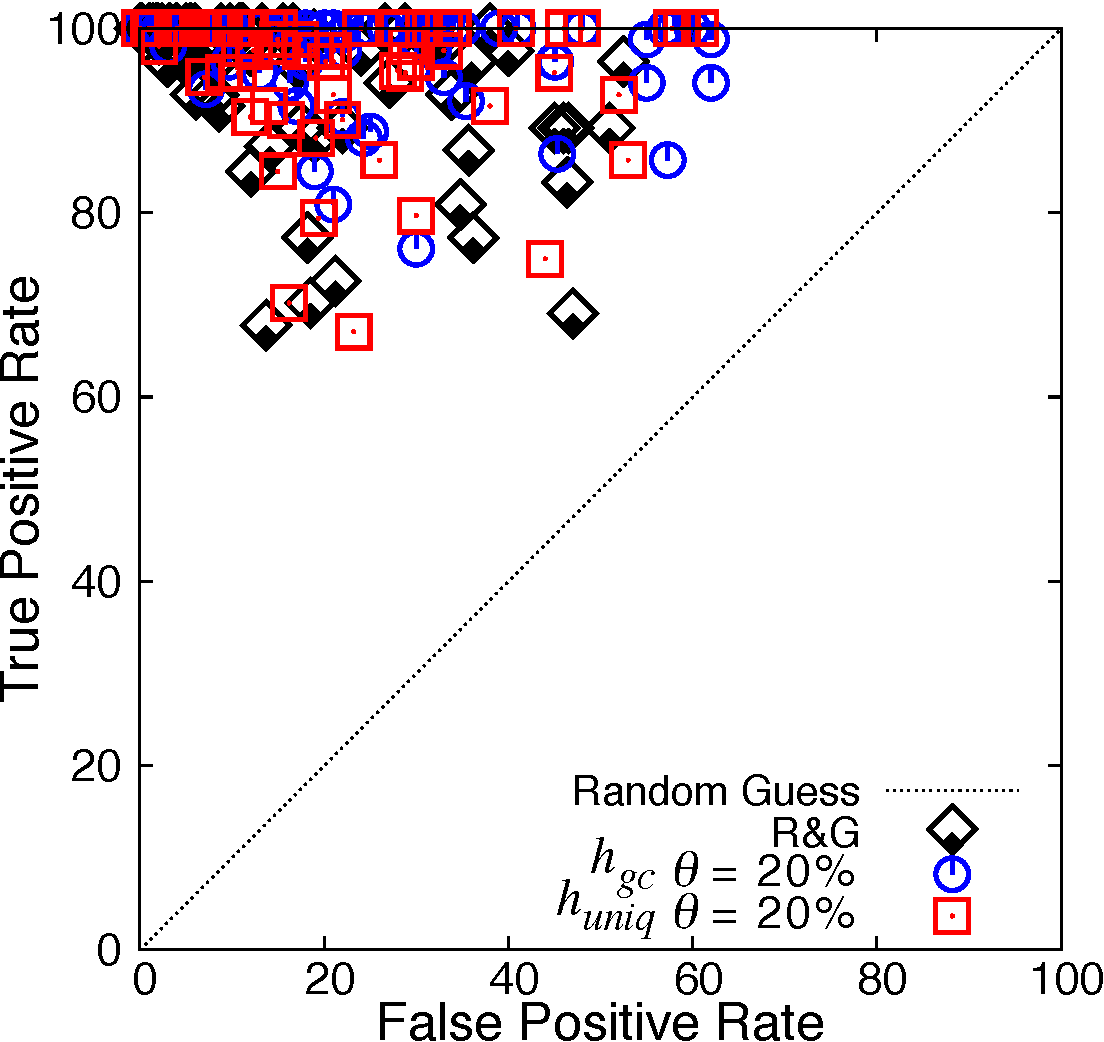
\includegraphics[width=0.6\linewidth]{fig/rocspace-all_domains.pdf}
% 	\end{figure}
% \end{frame}
%
% % @@@@@@@@@@@@@@@@@@@@@@@@@@@@@@@@@@@@@@@@@@@@@@@@@@@@@@@@@@@@@@@
% \begin{frame}{Experiments and Evaluation - Recognition Time}
% 	\begin{figure}[here]
% 		\centering
% 		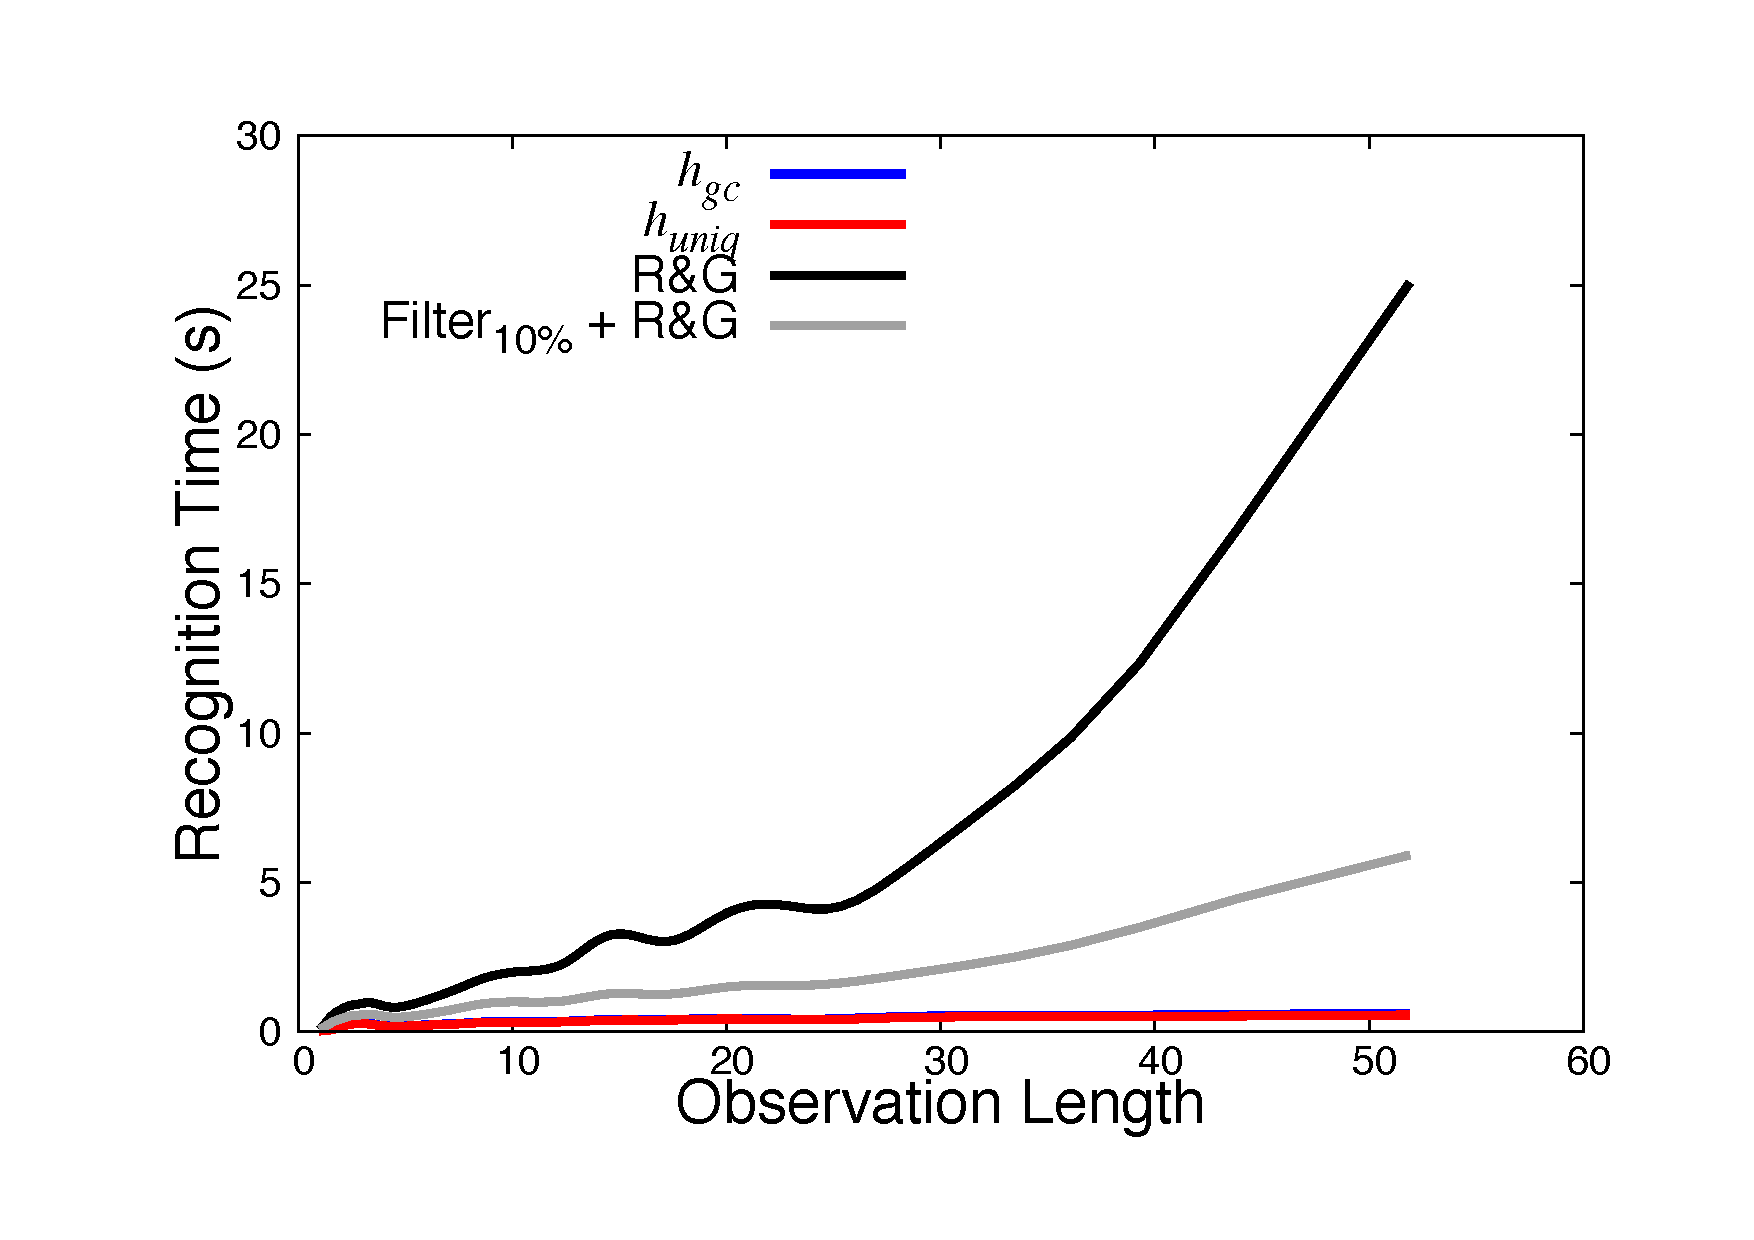
\includegraphics[width=0.7\linewidth]{fig/missing-recognition_time.pdf}
% 	\end{figure}
% \end{frame}
%
% \begin{frame}{Experiments and Evaluation - Recognition Time with Noise}
% 	\begin{figure}[here]
% 		\centering
% 		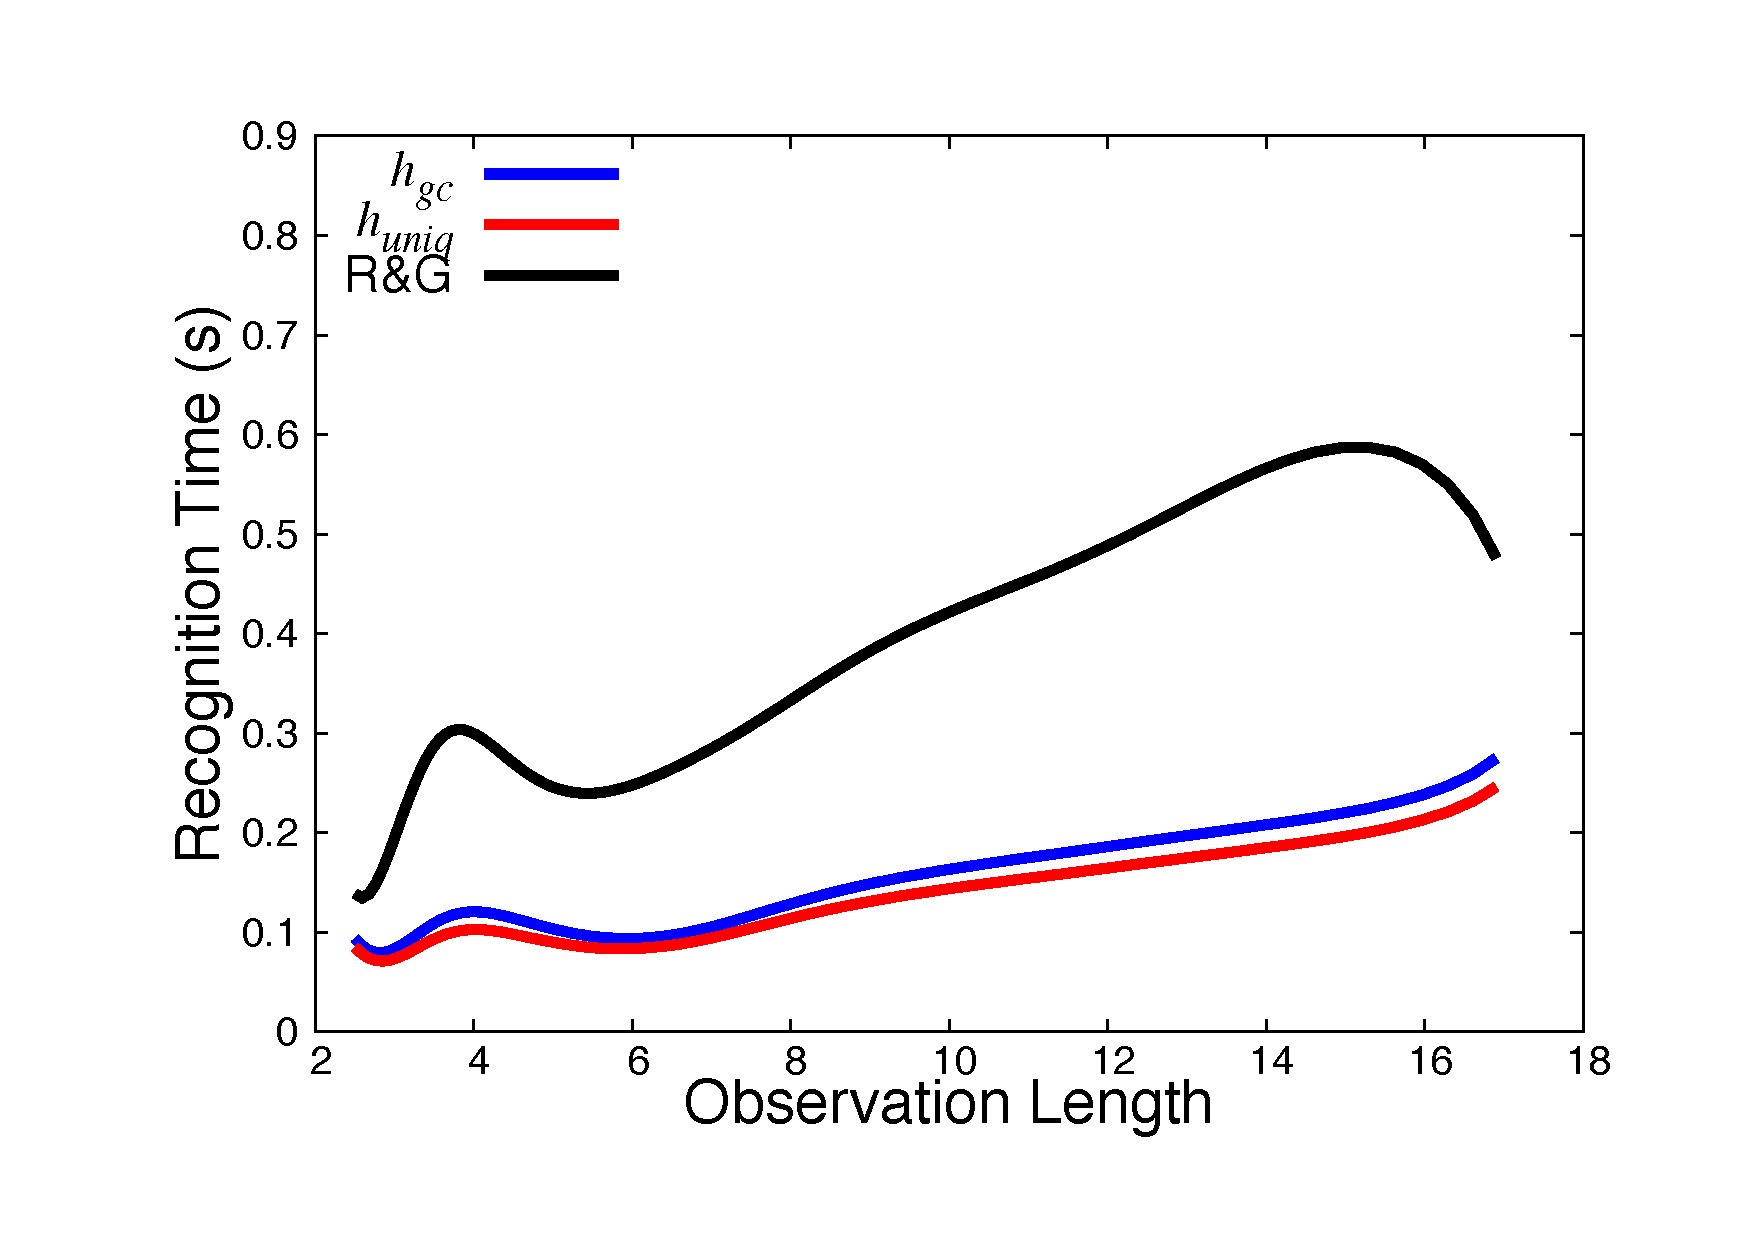
\includegraphics[width=0.7\linewidth]{fig/noisy-recognition_time.pdf}
% 	\end{figure}
% \end{frame}
%
%
% %---------------------------------------------------------------------------------
% 	% RFP - Do we need talk about related work?!
% 	% \begin{frame}{Related Work}
% 	% 	\begin{itemize}
% 	% 		\item ?
% 	% 	\end{itemize}
% 	% \end{frame}
%
% %---------------------------------------------------------------------------------
%
% \begin{frame}{Contributions and Limitations}
% % 	\todo{REDO THIS SLIDE}
%    	\begin{itemize}
%    		\item \textbf{Contribution so far:}
% 			\begin{itemize}
% 				\item Use planning landmarks for goal recognition;
% 				\item Obviate the need to run a planner during goal recognition, resulting in much faster and highly accurate recognition; and
%                 \item Robust dataset to evaluate goal recognition algorithms
% 			\end{itemize}
% 		% \item We show that our heuristics are more accurate and much faster than Ramírez and Geffner's approach ({\footnotesize Plan Recognition as Planning. IJCAI, 2009}).
% 		\item \textbf{Limitations:}
% 			\begin{itemize}
% 				\item Sensitive to the presence of landmarks; and
% 				\item Low accuracy with very few observations, \emph{i.e.}, 10\% of observability;
% 			\end{itemize}
% % 		\item \textbf{Future Work:}
% % 			\begin{itemize}
% % 				\item Use different landmark extraction algorithms;
% % 				\item Use goal ordering techniques;
% % 				\item Derive a probabilistic interpretation for the landmarks; and
% % 				\item Apply our landmark-based heuristics to continuous and temporal domains.
% % 			\end{itemize}
% 	\end{itemize}
% \end{frame}
%
% %---------------------------------------------------------------------------------
% \section{Online Goal Recognition as Reasoning over Landmarks}
%
% 	\begin{frame}[c]\frametitle{Motivation for Efficient Online Goal Recognition}
% 		Most goal recognition approaches using domain models have three key limitations:
% 		\begin{enumerate}
% 			\item assumption of a discrete state-space in a PDDL-like formalism
% 			\begin{itemize}
% 				\item not viable for use with path planning scenarios
% 			\end{itemize}
% 			\item assume all access to all observations at once
% 			\begin{itemize}
% 				\item approaches do not consider the time to recognition
% 			\end{itemize}
% 			\item need to call a planner multiple times per goal to rank hypotheses
% 			\begin{itemize}
% 				\item PRAP is computationally expensive, impractical for long plans
% 			\end{itemize}
% 		\end{enumerate}
% 	\end{frame}
%
% 	\begin{frame}[c]\frametitle{Online vs. Offline Plan Recognition}
% 		\begin{itemize}
% 			\item Offline plan recognition:
% 			\begin{itemize}
% 				\item All observations received at once;
% 				\item Observations may be incomplete or noisy;
% 				\item One-shot recognition;
% 			\end{itemize}
% 			\item Online plan recognition:
% 			\begin{itemize}
% 				\item Observations received incrementally;
%                 \item Observations may be incomplete or noisy; %(can use facts as observations);
% 				\item Objective is to recognize goal as soon as possible, without the full observation sequence
% 			\end{itemize}
% 		\end{itemize}
% 		\begin{center}
% 			\vspace{-3mm}
% 			\includegraphics[width=.9\textwidth]{fig/observations-example.pdf}
% 		\end{center}
% 	\end{frame}
%
% 	\begin{frame}[c]\frametitle{Efficient Online Goal Recognition}
% 		% Thus, want to develop an approach that can:
% % 		\begin{itemize}
% % 			\item recognize plans over continuous and discrete domains
% % 			\item use a full-fledged planner as little as possible
% % 			\item return reliable goal ranking as soon as possible
% % 		\end{itemize}
% 		Our approach:
% 		\begin{itemize}
% 			\item is efficient for online goal recognition;
% 			\item works in both discrete and continuous domains;
% 			\if\masterclass1
% 			\item uses goal-mirroring to minimize planner calls;
% 			\else
% 			\item minimizes planner calls;
% 			\fi
% 			\item reasons about landmarks to minimize the number of goal hypotheses;
% 			\item returns reliable goal ranking as soon as possible
% 		\end{itemize}
% 	\end{frame}
%
% \if\masterclass1
% 	\begin{frame}[c]\frametitle{Previous Work: Ramirez and Geffner}
% 		\if\masterclass1
% 		\todo{Move this to the background}
% 		\fi
% 		\begin{itemize}
% 			\item First approaches to goal recognition: Plan Recognition as Planning (PRAP)
% 			\item Probabilistic model aims to compute $P(G \mid O)$
% 			\item Following Bayes Rule $P(G \mid O) = \alpha P(O \mid G) P(G)$
% 			\item Given $P(G)$ as a prior, key bottleneck is computing $P(O \mid G)$
% 			\begin{itemize}
% 				\item In their work $P(O \mid G)$ is computed in terms of a cost difference $c(G,O) - c(G,\bar{O})$
% 				\item Computational cost is \textbf{two planner calls per goal hypothesis}
% 				\item For online recognition: two planner calls per goal hypothesis \textbf{per observation}
% 			\end{itemize}
% 			\item Some conclusions challenged for path planning domains\\ (Masters and Sardina 2017)
% 		\end{itemize}
% 	\end{frame}
%
% 	\begin{frame}[c]\frametitle{Previous Work: Goal Mirroring}
% 		\begin{itemize}
% 			\item Focuses on efficient online recognition
% 			\item Uses a planner to generate plan hypotheses using $(|O|+1)|G|$ planner calls
% 			\begin{itemize}
% 				\item Computes optimal plans for each goal
% 				\item For every incoming observation compute:
% 				\begin{itemize}
% 					\item prefix -- concatenation of observations
% 					\item suffix -- plan from last observation to every goal
% 				\end{itemize}
% 				\item Rank plan hypotheses by comparing to ideal plan
% 			\end{itemize}
% 		\end{itemize}
% 	\end{frame}
%
% 	\begin{frame}[c]\frametitle{Previous Work: Goal Recognition using Heuristics}
% 		\begin{itemize}
% 			\item Focuses on efficient recognition with \textbf{no planner calls}
% 			\item Uses heuristic estimation of states resulting from observation
% 			\item Ranks goals as a weighed sum based on the number of \textbf{landmarks} visited by the observations
% 			\item Key characteristics:
% 			\begin{itemize}
% 				\item Very fast (linear on the number of goals and observations)
% 				\item Less accurate in domains with few landmarks and/or observability
% 			\end{itemize}
% 		\end{itemize}
% 	\end{frame}
% \fi
%
% 	\if\masterclass1
% 	\begin{frame}[c]\frametitle{Domain formalization}
% 		The underlying representation adapts from the Transition Normal Form (TNF) (from Pommerening and Helmert), specifically
% 		\begin{itemize}
% 			\item Domain model originally dealt with operators that modify the truth-value of \emph{facts} or fluents
% 			\item We adopt a domain model $M = \langle \mathcal{V}, \mathcal{O} \rangle$:
% 			\begin{itemize}
% 				\item $\mathcal{V}$ is a set of variables with a, possibly infinite, domain
% 				\item operators in $\mathcal{O}$ change the value of all variables in $\mathcal{V}$ from $s$ into $s'$
% 				\item $cost(o)$ is usually $1$, but when dealing with continuous variables it is the euclidean distance of such values between $s$ and $s'$
% 			\end{itemize}
% 		\end{itemize}
% 	\end{frame}
%
% 	\begin{frame}[c]\frametitle{Landmarks in Discrete Domains}
% 		\begin{columns}
% 			\begin{column}{0.5\textwidth}
% 				\begin{itemize}
% 					\item Facts that must be true in all valid plans
% 					\item Root node is the goal condition
% 					\item Leaves are facts of initial state
% 					\item Connected boxes – facts that must be true together
% 				\end{itemize}
% 			\end{column}
% 			\begin{column}{0.5\textwidth}
% 				\includegraphics[width=\textwidth]{fig/blocksworld-landmarks-example.pdf}
% 			\end{column}
% 		\end{columns}
% 	\end{frame}
% 	\fi
%
% 	\begin{frame}[c]\frametitle{Landmarks in Continuous Domains}
% 		We need a notion of landmark in continuous domains
% 		\begin{columns}
% 			\begin{column}{0.7\textwidth}
% 			\begin{itemize}
% 				\item Redefine landmarks as areas surrounding goals
% 				\begin{itemize}
% 					\item Goals – Black dots
% 					\item Surrounding Rectangles – continuous landmark areas
% 				\end{itemize}
% 				\item To reach a goal the observed motion must intersect (go through) the corresponding landmark area.
% 				\item In this work, landmark areas roughly correspond to rooms partitioned as rectangular Voronoi diagrams
% 				\begin{itemize}
% 					\item Other notions of numeric landmarks may apply \\(e.g. Scala et al. IJCAI 2017)
% 				\end{itemize}
% 			\end{itemize}
% 			\end{column}
% 			\begin{column}{0.3\textwidth}
% 			\includegraphics[width=\textwidth]{fig/continuous-landmark-example.pdf}
% 			\end{column}
% 		\end{columns}
% 	\end{frame}
%
% 	\if\masterclass1
% 	\begin{frame}[c]\frametitle{Extracting Landmarks in Continuous Domains}
% 		\todo{Finish this for the masterclass}
% 	\end{frame}
% 	\fi
%
% 	\begin{frame}[c]\frametitle{Online Recognition with Landmarks}
% 		\begin{columns}
% 			\begin{column}{0.7\textwidth}
% 			\begin{itemize}
% 				\item Generate the ordered set of achieved landmarks
% 				\item Maintain the group of goals eliminated due to landmarks
% 				\item For every observation:
% 				\begin{itemize}
% 					% \item Check if it caused any landmarks to be achieved
% 					\item Check if it ``achieved'' a landmark
% 					% \item Intersect observation point with landmark areas
% 					\item If observations backtrack, re-instate goals
% 				\end{itemize}
% 				\item Rank goals using the landmark completion heuristic $h_{gc}$
% 			\end{itemize}
% 			\end{column}
% 			\begin{column}{0.3\textwidth}
% 				\includegraphics[width=\textwidth]{fig/continuous-landmark-example.pdf}
% 			\end{column}
% 		\end{columns}
% 	\end{frame}
%
% 	\if\masterclass1
% 	\begin{frame}[c]\frametitle{Online Recognition with Landmarks}
% 		\todo{For masterclass, put algorithm with example}
% 	\end{frame}
% 	\fi
%
% 	\begin{frame}[c]\frametitle{Goal Mirroring with Landmarks}
% 		Combines landmark reasoning with goal mirroring
% 		\begin{columns}
% 			\begin{column}{0.7\textwidth}
% 			\begin{itemize}
% 				\item Compute landmarks and optimal plans for all goals
% 				\item For every observation:
% 				\begin{itemize}
% 					\item Compute plan prefix, and for every goal
% 					\begin{itemize}
% 						\item Either prune goals that have \textbf{passed} the last landmark; or
% 						\item Compute plan suffix (from last observation) using planner
% 						\item Compute \textbf{cost ratio} between prefix+suffix and optimal plan
% 					\end{itemize}
% 				\end{itemize}
% 				\item Rank unpruned goals based on a \textbf{normalized cost ratio}
% 			\end{itemize}
% 			\end{column}
% 			\begin{column}{0.3\textwidth}
% 				\includegraphics[width=\textwidth]{fig/continuous-landmark-example.pdf}
% 			\end{column}
% 		\end{columns}
% 		\begin{itemize}
% 			\item Ranks $P(g_k \mid O)$ using a normalizing factor $\eta 1/\sum_{g_k \in G} rank(g_k)$
% 			\item Approximates $P(g \mid O) = \eta \sum_{g_k \in G} P(O \mid g_k) P(g_k)$ for all goals, assuming $P(g_k) = 0$ for pruned goals
% 		\end{itemize}
% 	\end{frame}
%
% 	\if\masterclass1
% 	\begin{frame}[c]\frametitle{Goal Mirroring with Landmarks}
% 		\todo{Algorithm and example for masterclass}
% 	\end{frame}
% 	\fi
%
% \if\masterclass1
% 	\begin{frame}[c]\frametitle{Continuous Evaluation}
% 		\begin{columns}
% 			\begin{column}{0.7\textwidth}
% 				\begin{itemize}
% 					\item Cubicles environment and robot (OMPL)
% 					\item 11 points spread evenly over the environment
% 					%\item Two different paths from start to goal 110*2 problems
% 					\item 220 problems
% 				\end{itemize}
% 		\end{column}
% 		\begin{column}{0.3\textwidth}
% 			\includegraphics[width=\textwidth]{fig/CubiclesEnv_RobotOnlyView.png}
% 		\end{column}
% 		\end{columns}
% 	\end{frame}
% \fi
%
% \if\masterclass1
% 	\begin{frame}[c]\frametitle{Discrete Evaluation}
% 		\begin{columns}
% 			\begin{column}{0.7\textwidth}
% 				\begin{itemize}
% 					\item Dataset expanded from Ramirez and Geffner's original work
% 					\item Domains extracted from the IPC competition
% 					\item Hundreds of goal recognition problems
% 				\end{itemize}
% 			\end{column}
% 			\begin{column}{0.3\textwidth}
% 			Domains
% 			\begin{itemize}
% 				\tiny
% 				\item \textsc{Blocks-World}
% 				\item \textsc{Campus}
% 				\item \textsc{Depots}
% 				\item \textsc{Driver-Log}
% 				\item \textsc{Dock-Worker-Robots}
% 				\item \textsc{Easy-IPC-Grid}
% 				\item \textsc{Ferry}
% 				\item \textsc{Intrusion-Detection}
% 				\item \textsc{Kitchen}
% 				\item \textsc{Logistics}
% 				\item \textsc{Miconic}
% 				\item \textsc{Rovers}
% 				\item \textsc{Satellite}
% 				\item \textsc{Sokoban}; and
% 				\item \textsc{Zeno-Travel}
% 			\end{itemize}
% 			\end{column}
% 		\end{columns}
% 	\end{frame}
% \fi
%
% \if\masterclass1
% 	\begin{frame}[c]\frametitle{Performance Results}
% 		\todo{Redo this table for the masterclass}
% 		\newcommand{\timeout}{\fontsize{4}{4}\selectfont \textit{Timeout}}
% 		\tiny
% 		\begin{tabular}{llll|cccccc|cccccc|cccccc|}
% 		\cline{5-22}
% 		                                                                                              &                                &                                &               & \multicolumn{18}{c|}{\bf Continuous Domains}                                                                                                                                      \\ \cline{5-22}
% 		                                                                                              &                                &                                &               & \multicolumn{6}{c|}{\sc Goal Mirroring}
% 		& \multicolumn{6}{c|}{\sc Goal Mirroring with Landmarks}
% 		& \multicolumn{6}{c|}{\sc Online Recognition with Landmarks}                                                            \\ \hline
% 		\multicolumn{1}{|c|}{\textit{\begin{tabular}[c]{@{}c@{}}Domain\\ (\# problems)\end{tabular}}\hspace{0.2em}}
% 		& \multicolumn{1}{c}{\textit{$|G|$}} & \multicolumn{1}{c}{\textit{$|O|$}} & \multicolumn{1}{c|}{\textit{$|L|$}}
% 		& \textit{Time}     & \textit{PC} & \textit{TPR} & \textit{FPR} & \textit{RF} & \textit{CV}
% 		& \textit{Time}     & \textit{PC} & \textit{TPR} & \textit{FPR} & \textit{RF} & \textit{CV}
% 		& \textit{Time}     & \textit{PC} & \textit{TPR} & \textit{FPR} & \textit{RF} & \textit{CV} \\ \hline
%
% 		\multicolumn{1}{|c|}{\begin{tabular}[c]{@{}c@{}}Cubicles\\ (220)\end{tabular}\hspace{0.2em}}
% 			& \multicolumn{1}{c}{11.0}
% 			& \multicolumn{1}{c}{26.5}
% 			& \multicolumn{1}{c|}{11.0}
% 			% Mirroring Results
% 			& 104.70	& 265.0		& \textbf{100\%}		& 100\%		& 20.2\%	& 21.8\%
%
% 			% Mirroring with Landmarks
% 			& 85.90 	& 184.8		& 78.2\%	& 61.1\%	& \textbf{24.3\%}	& \textbf{26.2\%}
%
% 			% Landmarks
% 			& \textbf{0.020}  & \textbf{0}	& 78.3\%	& \textbf{60.9\%}	& 21.7\%	&	15\% \hspace{0.3em}             \\ \hline
% 		\end{tabular}
%
% 		\vspace{1mm}
%
% 		\begin{tabular}{llll|cccccc|cccccc|cccccc|}
% 		\cline{5-22}
% 		                                                                                              &                                &                                &               & \multicolumn{18}{c|}{\bf Discrete Domains}                                                                                                                                      \\ \cline{5-22}
% 		                                                                                              &                                &                                &               & \multicolumn{6}{c|}{\sc Goal Mirroring}
% 		& \multicolumn{6}{c|}{\sc Goal Mirroring with Landmarks}
% 		& \multicolumn{6}{c|}{\sc Online Recognition with Landmarks}                                                            \\ \hline
% 		\multicolumn{1}{|c|}{\textit{\begin{tabular}[c]{@{}c@{}}Domain\\ (\# problems)\end{tabular}}}
% 		& \multicolumn{1}{c}{\textit{$|G|$}} & \multicolumn{1}{c}{\textit{$|O|$}} & \multicolumn{1}{c|}{\textit{$|L|$}}
% 		& \textit{Time}     & \textit{PC} & \textit{TPR} & \textit{FPR} & \textit{RF} & \textit{CV}
% 		& \textit{Time}     & \textit{PC} & \textit{TPR} & \textit{FPR} & \textit{RF} & \textit{CV}
% 		& \textit{Time}     & \textit{PC} & \textit{TPR} & \textit{FPR} & \textit{RF} & \textit{CV} \\ \hline
%
% 		\multicolumn{1}{|c|}{\begin{tabular}[c]{@{}c@{}}Campus\\ (15)\end{tabular}}
% 			& \multicolumn{1}{c}{2.0}
% 			& \multicolumn{1}{c}{5.4}
% 			& \multicolumn{1}{c|}{8.6}
% 			% Mirroring Results
% 			& 0.441		& 12.8	& 60.0\%	& 21.3\% 	& 57.3\% 	& 41.3\%
%
% 			% Mirroring with Landmarks
% 			& 0.212		& 7.7	& \textbf{96.4\%}	& \textbf{1.7\%}	& \textbf{96.4\%} 	& \textbf{96.4\%}
%
% 			% Landmarks
% 			& \textbf{0.065} & \textbf{0}	& 92.8\%	& 3.5\%		& 92.8\% 	& 92.8\%              \\ \hline
%
% 		\multicolumn{1}{|c|}{\begin{tabular}[c]{@{}c@{}}IPC-Grid\\ (61)\end{tabular}}
% 			& \multicolumn{1}{c}{8.3}
% 			& \multicolumn{1}{c}{21.8}
% 			& \multicolumn{1}{c|}{10.2}
% 			% Mirroring Results
% 			& 10.36		& 209.1		& \textbf{87.2\%}	& 19.4\%	& 36.6\% 	& 35.6\%
%
% 			% Mirroring with Landmarks
% 			& 3.29		& 71.2		& 55.6\%	& \textbf{10.5\%} 	& \textbf{45.8\%}	& \textbf{41.5\%}
%
% 			% Landmarks
% 			& \textbf{0.335}	& \textbf{0}	& 59.4\%	& 21.8\% 	& 32.6\%	& 31.1\%              \\ \hline
%
% 		\multicolumn{1}{|c|}{\begin{tabular}[c]{@{}c@{}}Ferry\\ (28)\end{tabular}}
% 			& \multicolumn{1}{c}{7.5}
% 			& \multicolumn{1}{c}{24.2}
% 			& \multicolumn{1}{c|}{28.5}
% 			% Mirroring Results
% 			& 55.24	& 179.5		& 83.1\%	& 10.2\% 	& 59.2\%	& 57.2\%
%
% 			% Mirroring with Landmarks
% 			& 7.98	& 35.4		& \textbf{83.3\%}	& \textbf{3.1\%} 	& \textbf{82.4\%}	& \textbf{82.1\%}
%
% 			% Landmarks
% 			& \textbf{0.101}	& \textbf{0}		& 82.4\%	& 5.4\%  & 72.5\%	& 71.9\%              \\ \hline
%
% 		\multicolumn{1}{|c|}{\begin{tabular}[c]{@{}c@{}}Intrusion\\ (45)\end{tabular}}
% 			& \multicolumn{1}{c}{16.6}
% 			& \multicolumn{1}{c}{13.1}
% 			& \multicolumn{1}{c|}{16.0}
% 			% Mirroring Results
% 			& 2.02	& 235.5		& \textbf{100\%}		& 7.2\% 	& 55.3\%	& 55.3\%
%
% 			% Mirroring with Landmarks
% 			& 0.257	& 34.7		& 75.5\%	& \textbf{3.6\%} 	& \textbf{67.1\%}	& \textbf{67.1\%}
%
% 			% Landmarks
% 			& \textbf{0.127}	& \textbf{0}	& 87.6\%	& 3.9\% 	& 57.1\%	& 55.1\%              \\ \hline
%
% 		\multicolumn{1}{|c|}{\begin{tabular}[c]{@{}c@{}}Kitchen\\ (15)\end{tabular}}
% 			& \multicolumn{1}{c}{3.0}
% 			& \multicolumn{1}{c}{7.4}
% 			& \multicolumn{1}{c|}{5.0}
% 			% Mirroring Results
% 			& 0.141	& 25.4		& 70.1\%	& 18.4\% 	& 44.6\%	& 36.1\%
%
% 			% Mirroring with Landmarks
% 			& 0.07	& 20.0		& 77.6\%	& \textbf{17.9\%} 	& \textbf{62.6\%}	& \textbf{58.3\%}
%
% 			% Landmarks
% 			& \textbf{0.04}	& \textbf{0}	& \textbf{100\%}		& 50\% 		& 23.9\%	& 23.9\%              \\ \hline
%
% 		\multicolumn{1}{|c|}{\begin{tabular}[c]{@{}c@{}}Logistics\\ (61)\end{tabular}}
% 			& \multicolumn{1}{c}{10.4}
% 			& \multicolumn{1}{c}{24.4}
% 			& \multicolumn{1}{c|}{16.1}
% 			% Mirroring Results
% 			& 53.82	& 199.3		& \textbf{95.4\%}	& 14.7\% 	& 26.9\%	& 25.8\%
%
% 			% Mirroring with Landmarks
% 			& 14.39	& 49.6		& 61.7\%	& \textbf{6.7\%} 	& \textbf{49.1\%}	& \textbf{48.4\%}
%
% 			% Landmarks
% 			& \textbf{0.594}	& \textbf{0}	& 56.1\%	& 9.5\% 	& 40.5\%	& 40.5\%              \\ \hline
%
% 		\multicolumn{1}{|c|}{\begin{tabular}[c]{@{}c@{}}Rovers\\ (28)\end{tabular}}
% 			& \multicolumn{1}{c}{6.0}
% 			& \multicolumn{1}{c}{24.9}
% 			& \multicolumn{1}{c|}{19.8}
% 			% Mirroring Results
% 			& \timeout	& -	& -	& -	& - & -
%
% 			% Mirroring with Landmarks
% 			& 58.87	& 31.1		& \textbf{76.8\%}	& \textbf{4.8\%} 	& \textbf{76.2\%}	& \textbf{75.1\%}
%
% 			% Landmarks
% 			& \textbf{0.867}	& \textbf{0}	& 72.1\%	& 8.5\% 	& 62.1\%	& 62.1\%              \\ \hline
%
% 		\multicolumn{1}{|c|}{\begin{tabular}[c]{@{}c@{}}Satellite\\ (28)\end{tabular}}
% 			& \multicolumn{1}{c}{6.4}
% 			& \multicolumn{1}{c}{16.9}
% 			& \multicolumn{1}{c|}{10.1}
% 			% Mirroring Results
% 			& 93.89	& 177.2		& \textbf{100\%}		& 33.8\% 	& 36.1\%	& 36.1\%
%
% 			% Mirroring with Landmarks
% 			& 5.18	& 30.6		& 81.8\%	& 9.4\% 	& \textbf{72.8\%}	& \textbf{71.9\%}
%
% 			% Landmarks
% 			& \textbf{1.09}	& \textbf{0}	& 78.2\%	& \textbf{9.3\%} 	& 64.4\%	& 64.1\%              \\ \hline
% 		\end{tabular}
% 	\end{frame}
% \fi
%
% 	\begin{frame}[c]\frametitle{Performance Results}
% 		\begin{center}
% 			\includegraphics[width=.8\textwidth]{roc_space-online_approaches/rocspace-all_domains-online.pdf}
% 		\end{center}
% 	\end{frame}
%
% 	\begin{frame}[c]\frametitle{Efficiency Results}
% 		\begin{center}
% 			\includegraphics[width=.45\textwidth]{fig/histogram-number_of_calls_to_planner.pdf}
% 			\includegraphics[width=.45\textwidth]{fig/histogram-time_improvement_percent.pdf}
% 		\end{center}
% 	\end{frame}
%
% 	\begin{frame}[c]\frametitle{Contributions and Limitations}
%    	\begin{itemize}
%    		\item \textbf{Contribution so far:}
% 			\begin{itemize}
% 				\item Extended de idea of landmarks for continuous domains; and
% 				\item Developed online algorithms able to recognize plans in\\ discrete and continuous domains;
% 				\item \textbf{Very} efficient in both discrete and continuous domains.
% 			\end{itemize}
% 		% \item We show that our heuristics are more accurate and much faster than Ramírez and Geffner's approach ({\footnotesize Plan Recognition as Planning. IJCAI, 2009}).
% 		\item \textbf{Limitations:}
% 			\begin{itemize}
% 				\item Naive notion of spatial landmarks;
% 				\item Much better performance on discrete domains.
% 			\end{itemize}
% % 		\item \textbf{Future Work:}
% % 			\begin{itemize}
% % 				\item Use different landmark extraction algorithms;
% % 				\item Use goal ordering techniques;
% % 				\item Derive a probabilistic interpretation for the landmarks; and
% % 				\item Apply our landmark-based heuristics to continuous and temporal domains.
% % 			\end{itemize}
% 	\end{itemize}
% 	\end{frame}
%
% %---------------------------------------------------------------------------------
%
% \if\masterclass1
% \section{Goal Recognition in Incomplete Domains}
%
% \if\masterclass0
% 	\begin{frame}[c]\frametitle{Masterclass}
% 		\begin{center}
% 			\large
% 			\todo{Come to the master class in Aberdeen for this!!}
% 		\end{center}
% 	\end{frame}
% \fi
%
% \if\masterclass1
% \begin{frame}[c]\frametitle{Motivation}
% 	\todo{This goes into the masterclass}
% \end{frame}
% \fi
%
% \fi
%
% %---------------------------------------------------------------------------------
%
% \section{Real World Applications}
%
% \if\masterclass1
% \subsection{Optimality Monitoring and Plan Abandonment}
% \begin{frame}[c]\frametitle{Optimality Monitoring}
%    	\begin{itemize}
%    		\item Agents often \textbf{deviate} from the optimal plan for multiple reasons
% 		\begin{itemize}
% 			\item they have concurrent/multiple goals; or
% 			\item they are not perfect optimizers;
% 		\end{itemize}
% 		\item We would like to be able to detect which actions in a plan do not advance (are non-optimal) towards a monitored goal;
% 		\item Our contribution is twofold:
% 			\begin{itemize}
% 				\item We formalize this problem using \textbf{planning domain definition}; and
% 				\item We combine two planning techniques to solve this problem: \textbf{landmarks} and \textbf{domain-independent heuristics}.
% 			\end{itemize}
% 		\item We evaluate our approach using several planning domains, and show that our approach yields \textbf{high accuracy} at \textbf{low computational cost}.
% 	\end{itemize}
% \end{frame}
%
% %---------------------------------------------------------------------------------
%
% \begin{frame}[c]\frametitle{Background: Planning, Heuristics, and Landmarks}
% 	\vspace{-2mm}
% 	\begin{definition}[Planning]
% 		A planning instance is represented by a triple $\Pi = \langle \Xi, \mathcal{I}, G\rangle$, in which:
% 		\begin{itemize}
% 			\item $\Xi= \langle \Sigma, \mathcal{A}\rangle$ is the \textbf{domain definition}, and consists of a finite set of \textbf{facts} $\Sigma$ and a finite set of \textbf{actions} $\mathcal{A}$ (action costs $=$ 1);
% 			\item $\mathcal{I}$ and $G$ represent the \textbf{planning problem}, in which $\mathcal{I}$ $\subseteq$ $\Sigma$ is the \textbf{initial state}, and $G$ $\subseteq$ $\Sigma$ is the \textbf{goal state}.
% 		\end{itemize}
% 	\end{definition}
% 	\vspace{-3mm}
% 	\begin{itemize}
% 		\item \textbf{Heuristics} are used to estimate the cost to achieve a particular goal. In this work, we use \textbf{domain-independent heuristics};
% 	\end{itemize}
% 	\vspace{-3mm}
% 	\begin{definition}[Landmarks]
% 		Given a planning instance $\Pi = \langle \Xi, \mathcal{I}, G\rangle$, a \textbf{fact} (or \textbf{action}) $L$ is a landmark in $\Pi$ iff $L$ 	must be \textbf{satisfied} (or \textbf{executed}) at some point along all valid plans that achieve $G$ from $\mathcal{I}$.
% 	\end{definition}
% \end{frame}
%
% %---------------------------------------------------------------------------------
%
% \begin{frame}[c]\frametitle{Plan Optimality Monitoring Problem}
% 	\begin{definition}[Plan Optimality Monitoring Problem]
% 		\begin{itemize}
%    			\item Domain definition (Facts and Actions) $\Xi$ $=$ $\langle \Sigma, \mathcal{A} \rangle$;
%    			\item Initial state \textbf{$\mathcal{I}$};
%    			\item A monitored goal $G$; and
%    			\item An observation sequence $O = \langle o_1, o_2, ..., o_n \rangle$, representing a full observable plan execution;
%    		\end{itemize}
% 	\end{definition}
%     % FRM - I'm not sure I like the sentence below, I will try to rephrase it
% 	\begin{itemize}
% 		\item The solution to a plan optimality monitoring problem is the set of observations (\textbf{non-optimal actions}) that do not advance an optimal plan that the agent may be following.
% 	\end{itemize}
% \end{frame}
%
% \begin{frame}[c]\frametitle{Roboschool Example}
% 	\todo{Complete with the Roboschool example}
% \end{frame}
%
% %---------------------------------------------------------------------------------
% \begin{frame}[c]\frametitle{Plan Optimality Monitoring Approach}
%    	\begin{itemize}
%    		\item Our approach \textbf{combines planning techniques}, \textit{i.e.}, landmarks and domain-independent heuristics.
% 		\item We use \textbf{landmarks} to obtain information about \textbf{what cannot be avoided} to achieve a monitored goal $G$; and
% 		\item We use \textbf{heuristics} to analyze possible \textbf{plan execution deviation}.
% 	\end{itemize}
% \end{frame}
% \begin{frame}[c]\frametitle{Analyzing Plan Execution Deviation}
%    	\begin{itemize}
% 		\item If an observation $o_i$ results a state $s_i$, we consider a \textbf{deviation from a plan} to occur if $h(s_{i-1}) < h(s_i)$.
%    	\end{itemize}
%   	\begin{figure}[here]
% 		\includegraphics[width=0.85\linewidth]{fig/plan_execution-deviation.pdf}
% 	\end{figure}
% \end{frame}
% %---------------------------------------------------------------------------------
% \begin{frame}[c]\frametitle{Predicting Non-regressive Actions via Landmarks}
% 	\begin{itemize}
% 		\item To predict which actions could be executed in the next observation, we \textbf{analyze the closest landmarks by estimating the distance} (using $h_{max}$) from the current state to the extracted landmarks $\mathcal{L}$, namely:
% 			\begin{itemize}
% 				\item For every fact landmark $l \in \mathcal{L}$ in which the estimated \textbf{distance is 0},we select those actions $a \in \mathcal{A}$ such that $l \in \textit{pre}(a)$; and
% 				\item For every fact landmark $l \in \mathcal{L}$ in which the estimated \textbf{distance is 1}, we select those actions $a \in \mathcal{A}$ such that $pre(a) \in$ current state and $l \in \textit{eff}(a)^+$;
% 			\end{itemize}
% 		\item These predicted actions \textbf{may reduce the distance} to the \textbf{monitored goal} and \textbf{next landmarks}.
% 	\end{itemize}
% \end{frame}
%
% \begin{frame}[c]\frametitle{Finding Non-regressive actions}
% 	% \todo{Possibly avoid this slide}
%     \begin{algorithmic}[1]
% 		\Require{$\Xi = \langle \Sigma, \mathcal{A} \rangle$ \textit{planning domain}, $\delta$ \textit{current state}, and $\mathcal{L}$ \textit{ordered fact landmarks}}
%         \Function{NonRegressiveActions}{$\Xi$, $\delta$, $\mathcal{L}$}
%         		\State $\eta_{PActions} \gets \langle$ $\rangle$
% 			\For{each fact landmark $l$ in $\mathcal{L}$} \label{alg:predictiNextActions:for}
% 				\State $Al \gets \langle \rangle$
%             		\If{$h_{max}(l) = 0$} \Comment{\footnotesize $h_{max}(l)$ \textit{estimates} $l$ \textit{from} $\delta$.} \label{alg:predictiNextActions:h0}
%             			\State $Al \gets$ all $a$ in $\mathcal{A}$ s.t. $l \in \textit{pre}(a)$ \label{alg:predictiNextActions:now}
% 				\ElsIf{$h_{max}$($l$) $=$ 1} \label{alg:predictiNextActions:h1}
% 					\State $Al \gets$ all $a \in \mathcal{A}$ s.t $\textit{pre}(a) \in \delta \land l \in \textit{eff}(a)^+$\label{alg:predictiNextActions:next}
% 				\EndIf
% 				\State $\eta_{PActions}$ := $\eta_{PActions}$ $\cup$ $Al$
%             \EndFor
%             	\State \textbf{return} $\eta_{PActions}$ \Comment{set of possible upcoming actions}
%         \EndFunction
%     \end{algorithmic}
% \end{frame}
%
% %---------------------------------------------------------------------------------
% \begin{frame}[c]\frametitle{Detecting Sub-Optimal Steps}
%
% 	\begin{itemize}
% 		\item To detect sub-optimal steps (actions) in observation sequence $O$ for a monitored goal $G$, we combine the techniques we developed and filter with the following condition:
% 			\begin{itemize}
%             	\item \textbf{An observed action $o \in O$ is considered sub-optimal if}: \\ $o$ $\notin$ set of predicted actions AND ($h(s_{i-1}) < h(s_i)$).
% 			\end{itemize}
% 	\end{itemize}
% \end{frame}
%
%
% \begin{frame}[c]\frametitle{Detecting Sub-Optimal Steps (Monitor Plan Optimality)}
% 	% \vspace{-3mm}
% %   	\begin{figure}[here]
% % 		\includegraphics[width=0.73\linewidth]{algo-monitor_planoptimality.png}
% % 	\end{figure}
%     \begin{algorithmic}[1]
% 		\Require{$\Xi = \langle \Sigma, \mathcal{A}, \rangle$ \textit{planning domain}, $\mathcal{I}$ \textit{initial state}, $G$ \textit{monitored goal}, and $O$ \textit{observed actions}.}
% 		% \Ensure{$A_{SubOptimal}$ \textit{as sub-optimal actions}.}
%         \Function{MonitorPlanOptimality}{$\Xi$,$\mathcal{I}$,$G$,$O$}
%         		\State $A_{SubOptimal} \gets \langle\rangle$ \Comment{\footnotesize \textit{Non-contributing actions towards goal} $G$.}
%         		\State $L \gets $ \textsc{ExtractLandmarks($\mathcal{I}$, $G$)}
% 			\State $\delta \gets \mathcal{I}$ \Comment{\footnotesize $\delta$ \textit{is the current state.}}
% 			\State $\eta_{PActions} \gets $ \textsc{NonRegressiveActions}($\Xi$, $\delta$, $L$)
% 			\State $D_{G} \gets$ \textsc{EstimateGoalDistance}($\delta$, $G$) \Comment{\footnotesize{\textit{Any domain-independent heuristic}}}
%         		\For{each observed action $o$ in $O$}
%         			\State $\delta \gets \delta$.\textsc{Apply}($o$)
%         			\State $D'_{G} \gets$ \textsc{EstimateGoalDistance}($\delta$, $G$)
%         			\If{$o$ $\notin$ $\eta_{PActions}$ $\wedge$ $(D'_{G} > D_{G})$}\label{alg:monitor:estimatesuboptimalstep}
%               		\State $A_{SubOptimal} \gets A_{SubOptimal} \cup o$
%             		\EndIf
% 				\State $\eta_{PActions} \gets$ {\textsc{NonRegressiveActions}($\Xi$, $\delta$, $L$)}
%         			\State $D_{G} \gets D'_{G}$
%         		\EndFor
%         		\State \textbf{return} $A_{SubOptimal}$
%         \EndFunction
%     \end{algorithmic}
% \end{frame}
%
% %---------------------------------------------------------------------------------
% \begin{frame}[c]\frametitle{Experiments and Evaluation (1 of 2)}
%    	\begin{itemize}
%    		\item We evaluate our approach over 10 planning domains;
% 		\begin{itemize}
% 			\item Precision: percentage of correctly detected sub-optimal steps;
% 			\item Recall: percentage of true sub-optimal steps, actually detected.
% 			% Here, a false negative is a sub-optimal action that is not detected by our approach. Recall provides the percentage of positive cases that our approach has detected.
% 		\end{itemize}
% 		\item We use 6 domain-independent heuristics:
% 		\begin{itemize}
% 			\item $h_{adjsum}$, $h_{adjsum2}$, $h_{adjsum2M}$, $h_{combo}$, $h_{ff}$, and $h_{sum}$;
% 		\end{itemize}
% 		\item To extract landmarks and their ordering, we use an algorithm developed by Hoffman \emph{et al.} {\footnotesize (Ordered Landmarks in Planning. JAIR, 2004)};
% 		\item We manually generate the dataset from medium and large planning problems, containing both optimal and sub-optimal plan execution.
% 	\end{itemize}
% \end{frame}
%
% \begin{frame}[c]\frametitle{Experiments and Evaluation (2 of 2)}
% 	\begin{table}[]
% 		\scriptsize
% 		\centering
% 		\begin{tabular}{|c|c|c|c|cc|}
% 		\hline
% 		\textbf{Domain}             & $|O|$  & $|\mathcal{L}|$  & \textbf{Heuristic}          & \textbf{Time}        & \textbf{Precision / Recall / F1} \\ \hline
% 		\textsc{Blocks-World}  & 15.2 & 20.1 & $h_{adjsum2}$ / $h_{ff}$ 	& 0.19 / 0.21 & 100\% / 74.2\% / 85.2\%       \\ \hline
% 		\textsc{Driver-Log}    & 20.1 & 53.6 & $h_{adjsum2M}$            & 1.33        & 100\% / 100\% / 100\% 	  	  \\ \hline
% 		\textsc{Depots}        & 16.7 & 64.7 & $h_{adjsum2}$ / $h_{ff}$  & 1.22 / 1.43 & 81.2\% / 100\% / 89.6\%       \\ \hline
% 		\textsc{Easy-IPC-Grid} & 14.1 & 48.5 & $h_{adjsum2}$ / $h_{ff}$  & 0.77 / 0.86 & 100\% / 100\% / 100\%         \\ \hline
% 		\textsc{Ferry} 		  & 13.8 & 18.1 & $h_{adjsum}$ / $h_{sum}$  & 0.23 / 0.19 & 88.8\% / 78.5\% / 83.1\%        \\ \hline
% 		\textsc{Logistics}     & 20.8 & 24.0 & $h_{adjsum2}$ / $h_{ff}$  & 0.35 / 0.55 & 100\% / 91.3\% / 95.4\%       \\ \hline
% 		\textsc{Miconic}       & 18.1 & 19.4 & $h_{adjsum}$ / $h_{sum}$  & 0.29 / 0.21 & 100\% / 86.9\% / 93.1\%       \\ \hline
% 		\textsc{Satellite}     & 25.7 & 60.8 & $h_{adjsum2M}$        	& 9.58 		  & 88.8\% / 53.3\% / 66.6\%       \\ \hline
% 		\textsc{Sokoban}       & 24.0 & 76.5 & $h_{combo}$           	& 4.28		  & 90.9\% / 83.3\% / 86.9\%       \\ \hline
% 		\textsc{Zeno-Travel}   & 12.2 & 38.7 & $h_{adjsum2}$ / $h_{ff}$  & 0.86 / 0.99 & 100\% / 92.8\% / 96.2\%       \\ \hline
% 		\end{tabular}
%         \caption{Plan Optimality Monitoring experimental (best) results.}
% 	\end{table}
% \end{frame}
%
% %---------------------------------------------------------------------------------
% \begin{frame}[c]\frametitle{Contributions and Limitations}
% 	% \todo{REDO THIS SLIDE}
%    	\begin{itemize}
%    		\item \textbf{Contribution:}
% 			\begin{itemize}
% 				\item Formalized plan optimality monitoring problem as planning;
% 				\item Developed an approach based on landmarks and heuristics;
% 				\item We show that our approach has high accuracy in almost all domains (besides \textsc{Satellite}).
% 			\end{itemize}
% 		\item \textbf{Limitations:}
% 			\begin{itemize}
% 				\item We do not yet deal with partial observability;
% 			\end{itemize}
% 		% \item \textbf{Future Work:}
% % 			\begin{itemize}
% %             	\item Evaluate our approach using more modern domain-independent heuristics;
% % 				\item Try/use different landmark extraction algorithms; and
% % 				\item Apply our approach to goal recognition (online and offline).
% % 			\end{itemize}
% 	\end{itemize}
% \end{frame}
% \fi
% %---------------------------------------------------------------------------------
%
% % ================================
% % = Plan recognition using video =
% % ================================
% \subsection{Plan Recognition using Video Data}
% % \begin{frame}[c]\frametitle{Plan Recognition using Video Data}
% % 	Get slides from Roger
% % \end{frame}
%
% \begin{frame}[c]
% 	\begin{center}
% 		\Large{Plan Recognition using Video Data}
% 	\end{center}
% \end{frame}
%
% \begin{frame}[c]\frametitle{Plan Recognition using Video Data}
% 	\begin{itemize}
%    		\item \textbf{Plan recognition}
%    		\begin{itemize}
% 				\item Task of recognizing the plan (i.e., the sequence of actions) the observed agent is following in order to achieve his intention (Sadri, 2012)
% 	    \end{itemize}
% 		\item \textbf{Activity recognition}
% 			\begin{itemize}
% 				\item The task of recognizing the independent set of actions that generates an interpretation to the movement that is being performed (Poppe,~2010)
% 				\item Such task is particularly challenging in the real physical world
% 			 \end{itemize}
% 		\item Much research effort focuses on activity and plan recognition as separate challenges;
% 		\item We develop a hybrid approach that comprises both activity and plan recognition;
% 		\item The approach infers, from a set of candidate plans, which plan a human subject is pursuing based exclusively on fixed-camera video.
% 	\end{itemize}
% 	\begin{flushright}
% 	{\tiny Poppe, R. A survey on vision-based human action recognition. \\Image and Vision Computing 28(6), pp. 976–990, 2010. \\
% 	       Sadri, Fariba. Intention Recognition in Agents for Ambient Intelligence: Logic-Based Approaches. \\ Ambient Intelligence and Smart Environments, pp. 197-236, 2012.
% 	}
% 	\end{flushright}
% \end{frame}
%
% \begin{frame}[c]\frametitle{A Hybrid Architecture for Activity and Plan Recognition}
%    	\begin{itemize}
%    		\item \textbf{Conceptually divided in two main parts}
%    		\begin{itemize}
% 				\item CNN-based activity recognition (CNN)
%                 \item CNN-backed symbolic plan recognition (SBR)
% 	    \end{itemize}
% 	\end{itemize}
% 	\begin{center}
% 		\includegraphics[width=0.8\linewidth]{fig/pipeline.pdf}
% 	\end{center}
% \end{frame}
%
% \if\masterclass1
% \begin{frame}[c]\frametitle{CNN-based Activity Recognition}
%    	\begin{itemize}
%    		\item \textbf{Convolutional Neural Network}
%    		\begin{itemize}
%    		    \item Architecture: GoogLeNet
% 			\item 22-layer deep network based on the Inception module
%             \item Input images: 224x224 (3 channels: RGB)
%             \item Output classes: 9 (activities)
% 	    \end{itemize}
%
% 	\end{itemize}
% \end{frame}
%
% \begin{frame}{CNN-backed Symbolic Plan Recognition}
%    	\begin{itemize}
%    		\item \textbf{Symbolic Behavior Recognition (SBR)}
%    		\begin{itemize}
% 				\item A plan recognition approach that takes as input a plan library and a sequence of observations
%                 \item Feature decision tree (FDT) maps observable features to plan-steps in a plan library
%                 \item SBR returns set of hypotheses plans such that each hypothesis represents a plan that achieves a top-level goal in a plan library
% 	    \end{itemize}
% 		\begin{center}
% 			\includegraphics[width=0.7\linewidth]{fig/fdt.pdf}
% 		\end{center}
% 	\end{itemize}
% \end{frame}
%
% \begin{frame}[c]\frametitle{CNN-backed Symbolic Plan Recognition}
%    	\begin{itemize}
%    		\item \textbf{Our Symbolic Behavior Recognition}
%    		\begin{itemize}
% 				\item We modify the SBR and replace the FDT with the CNN-backed Activity Recognition
%                 \item The CNN-backed Activity Recognition maps frames directly into nodes (activities) in the plan library used by SBR to compute sequential consistency of plan steps
% 	    \end{itemize}
% 		\begin{center}
% 			\includegraphics[width=0.9\linewidth]{fig/sbr.pdf}
% 		\end{center}
% 	\end{itemize}
% \end{frame}
% \fi
%
% \begin{frame}{Experiments: Dataset}
%    	\begin{itemize}
%    		\item ICPR 2012 Kitchen Scene Context based Gesture Recognition dataset (KSCGR)%\footnote{http://www.murase.m.is.nagoya-u.ac.jp/KSCGR/}
% 	    \item \textbf{5 recipes for cooking eggs in Japan}
%    		\begin{itemize}
% 				\item Ham and Eggs, Omelet, Scrambled-Egg, Boiled-Egg and Kinshi-Tamago
% 				\item Each recipe is performed by 7 subjects \\(5 in training set, 2 in testing set)
% 	    \end{itemize}
% 	    \item \textbf{9 cooking activities composes the dataset}
%    		\begin{itemize}
% 				\item Breaking, mixing, baking, turning, cutting, boiling, seasoning, peeling, and none
% 	    \end{itemize}
% 		\begin{figure}[here]
% 			\centering
% 			\includegraphics[width=0.7\linewidth]{fig/egg-dataset.pdf}
% 		\end{figure}
% 	\end{itemize}
% \end{frame}
%
% %---------------------------------------------------------------------------------
% \if\masterclass1
% \begin{frame}[c]\frametitle{Experiments: Plan Library Modeling}
%    	\begin{itemize}
% 		\item We model a plan library containing knowledge of the agent's possible goals and plans based on the KSCGR dataset
% 		\item We consider that a sequence of cooking gestures is analogous to a sequence of a plan in the plan library
% 		\begin{figure}[here]
% 			\centering
% 			\includegraphics[width=0.4\linewidth]{fig/boiledegg-kinshiegg.pdf}
% 		\end{figure}
% 	\end{itemize}
% \end{frame}
%
% %---------------------------------------------------------------------------------
% \iffalse
% \begin{frame}[c]\frametitle{Experiments}
%    	\begin{itemize}
%    		\item \textbf{Convolutional Neural Network}: GoogLeNet
% 		\item Experiments separated into training, validation and test phases
% 		\item \textbf{Training phase}
%    		\begin{itemize}
% 			\item Input images: 224x224
%             \item Training stops after 30 epochs
% 	    \end{itemize}
% 	    \item \textbf{Validation phase}
%    		\begin{itemize}
% 		    \item Select the model that achieves the highest accuracy
% 	    \end{itemize}
% 	    \item \textbf{Test phase}
%    		\begin{itemize}
% 			\item CNN classifies each frame from input assigning to the image a probability score for each class
% 	    \end{itemize}
% 	\end{itemize}
% \end{frame}
% \fi
% %---------------------------------------------------------------------------------
% \begin{frame}[c]\frametitle{Activity Recognition results}
% 	Precision, Recall, F-measure and Accuracy scores for each activity
% 	\begin{table}[tb!]
%         \centering
%         \footnotesize
%         \begin{tabular}{l|cccc}
%             \hline\noalign{\smallskip}
%             \textbf{Activity} & \textbf{Precision} & \textbf{Recall} & \textbf{F-measure} & \textbf{Accuracy} \\
%             \noalign{\smallskip}\hline\hline\noalign{\smallskip}
%             \textit{None}      &         0.65  & \textbf{0.97} &         0.78             &         0.64      \\
%             \textit{Breaking}  &         0.44  &         0.41  &         0.42             &         0.27      \\
%             \textit{Mixing}    &         0.67  &         0.34  &         0.45             &         0.29      \\
%             \textit{Baking}    &         0.74  &         0.88  & \textbf{0.80}            & \textbf{0.67}     \\
%             \textit{Turning}   &         0.77  &         0.38  &         0.51             &         0.34      \\
%             \textit{Cutting}   &         0.87  &         0.63  &         0.73             &         0.58      \\
%             \textit{Boiling}   &         0.61  &         0.34  &         0.43             &         0.28      \\
%             \textit{Seasoning} & \textbf{0.89} &         0.37  &         0.52             &         0.35      \\
%             \textit{Peeling}   &         0.72  &         0.10  &         0.18             &         0.09      \\
%             \noalign{\smallskip}\hline
%         \end{tabular}
%     \end{table}
% \end{frame}
%
%
% %---------------------------------------------------------------------------------
% \begin{frame}[c]\frametitle{Activity Recognition results}
% 	 Accuracy scores for each activity and the distribution of frames in KSCGR dataset
%
% 	\begin{minipage}{0.48\linewidth}
%         \begin{table}[tb!]
%             \centering
%             \footnotesize
%             \begin{tabular}{l|cc}
%                 \hline\noalign{\smallskip}
%                 \textbf{Activity} & \textbf{Frames} & \textbf{Accuracy} \\
%                 \noalign{\smallskip}\hline\hline\noalign{\smallskip}
%                 \textit{None}      & \textbf{31\%}  & \textbf{0.64}     \\
%                 \textit{Breaking}  &          3\%   &         0.27      \\
%                 \textit{Mixing}    &         11\%   &         0.29      \\
%                 \textit{Baking}    & \textbf{25\%}  & \textbf{0.67}     \\
%                 \textit{Turning}   &          5\%   &         0.34      \\
%                 \textit{Cutting}   &          9\%   &         0.58      \\
%                 \textit{Boiling}   &          7\%   &         0.28      \\
%                 \textit{Seasoning} &          3\%   &         0.35      \\
%                 \textit{Peeling}   &          6\%   &         0.09      \\
%                 \noalign{\smallskip}\hline
%             \end{tabular}
%         \end{table}
%     \end{minipage}
%     \begin{minipage}{0.48\linewidth}
%         \includegraphics[width=\linewidth]{fig/perc.pdf}
%     \end{minipage}
% \end{frame}
%
% %---------------------------------------------------------------------------------
% % True labels in columns and predicted labels in lines, thus:
% % The system should classify ``Breaking'' but instead some frames are classified as ``Peeling''
% \begin{frame}[c]\frametitle{Activity Recognition results}
% 	Confusion matrix
%
% 	\begin{minipage}{0.48\linewidth}
%         \includegraphics[width=\linewidth]{fig/egg-confusion_matrix.pdf}
%     \end{minipage}
%     \begin{minipage}{0.48\linewidth}
%         \includegraphics[width=0.8\linewidth]{fig/egg-cooking-similar.pdf}
%     \end{minipage}
%     \begin{itemize}
% 		\item Close position in the scene
%         \item Similar movements
%     \end{itemize}
% \end{frame}
%
% %---------------------------------------------------------------------------------
%
% \begin{frame}[c]\frametitle{Plan Recognition results}
%    	\begin{itemize}
% 		\item We evaluate the whole pipeline using the number of hypotheses inferred by the plan recognizer
%         \item \textbf{Score} weights correct predictions by the number of hypotheses
% 	\end{itemize}
%
% 	\begin{equation*}
%         Score = \frac{c}{\#recipesFromSBR}
%     \end{equation*}
%     \begin{itemize}
% 		\item c: 1 if the correct recipe was inferred, 0 otherwise
%         \item \#recipesFromSBR: Number of recipes yielded by the recognizer
%     \end{itemize}
% \end{frame}
%
% %---------------------------------------------------------------------------------
%
% \begin{frame}[c]\frametitle{Plan Recognition results}
%     \begin{center}
%         \scriptsize
%         \begin{tabular}{l|llc}
%             \hline\noalign{\smallskip}
%             \#                 & \textbf{True Recipe} & \textbf{Predicted Recipes} & \textbf{Score}\\
%             \noalign{\smallskip}\hline\hline\noalign{\smallskip}
%                               & Boiled-Egg   & Scramble-Egg, Omelette, Ham-Egg              & 0.00 \\
%                               & Ham-Egg      & Scramble-Egg, Omelette                       & 0.00 \\
%             10                & Kinshi-Egg   & Kinshi-Egg                                   & 1.00 \\
%                               & Omelette     & Scramble-Egg, Omelette                       & 0.50 \\
%                               & Scramble-Egg & Ham-Egg                                      & 0.00 \\
%             \noalign{\smallskip}\hline\hline\noalign{\smallskip}
%                               & Boiled-Egg   & Kinshi-Egg, Omelette, Ham-Egg                & 0.00 \\
%                               & Ham-Egg      & Scramble-Egg                                 & 0.00 \\
%             11                & Kinshi-Egg   & Scramble-Egg, Omelette, Ham-Egg              & 0.00 \\
%                               & Omelette     & Kinshi-Egg, Scramble-Egg, Omelette, Ham-Egg  & 0.25 \\
%                               & Scramble-Egg & Kinshi-Egg                                   & 0.00 \\
%             \noalign{\smallskip}\hline\hline\noalign{\smallskip}
%                                                         \multicolumn{3}{r}{\textbf{Average:}} & 0.18 \\
%             \noalign{\smallskip}\hline
%             \end{tabular}
%     \end{center}
% \end{frame}
% \fi
%
% %---------------------------------------------------------------------------------
% \iffalse
% \begin{frame}[c]\frametitle{Plan Recognition results}
%    	\begin{itemize}
% 			\item Some activity sequences occur only in test set and not in training set
%             \item Kinshi-Egg does not have any Turning activity in training set
%
%     		{\scriptsize
%     		\item[] \textbf{Dataset}: \#11 (testing set)
%     		\item[] \textbf{Recipe}: Kinshi-Egg
%     		\item[] \textbf{Activity sequence}: Breaking $\rightarrow$ Mixing $\rightarrow$ Baking $\rightarrow$ Turning $\rightarrow$ Baking $\rightarrow$ Cutting
%     		}
% 	\end{itemize}
%     \begin{itemize}
% 		\item Some sequences occur in more than one recipe in testing set
%         \item[]
%
% 		{\scriptsize
% 		\item[] \textbf{Dataset}: \#11 (testing set)
% 		\item[] \textbf{Recipe}: Scrambled-Egg and Omelette
% 		\item[] \textbf{Activity sequence}: Breaking $\rightarrow$ Cutting $\rightarrow$ Seasoning $\rightarrow$ Mixing $\rightarrow$ Baking $\rightarrow$ Mixing $\rightarrow$ Baking
% 		}
%     \end{itemize}
% \end{frame}
% \fi
%
% \if\masterclass0
% \begin{frame}[c]\frametitle{Summary of the Results}
% 	Conducted experiments on two levels:
% 	\begin{itemize}
% 		\item Activity Recognition
% 		\begin{itemize}
% 			\item Accuracy lower than 50\% (in 9-label classification) for infrequent activities
% 			\item Very good accuracy to identify ``no-action''
% 		\end{itemize}
% 		\item Overall Plan Recognition
% 		\begin{itemize}
% 			\item Low accuracy for overall plan recognition using plan-libraries
% 		\end{itemize}
% 	\end{itemize}
% \end{frame}
% \fi
%
% %---------------------------------------------------------------------------------
% \begin{frame}{Contributions and Future Work}
%    	\begin{itemize}
%    		\item We developed a hybrid architecture for activity and plan recognition
%         \item Pipeline includes:
%         \begin{itemize}
%             \item A CNN for activity recognition that feeds directly into:
%             \item a modified (SBR) approach that uses the CNN to index activities in the plan library
%         \end{itemize}
%
%         \item Approach limited by the plan library in the plan recognizer
%         \item Next steps:
% 		\begin{itemize}
% 			\item Employ other deep learning architectures such as Long-Short Term Memory networks (LSTM) and 3D CNNs
% 	        \item Use a more flexible approach for plan recognition, such as PRAP
% 	        \item Explore object recognition to provide additional clues of the activity that is being performed
% 		\end{itemize}
% 		\begin{center}
% 			Demo video: \url{https://youtu.be/BoiLjU1vg3E}
% 		\end{center}
%     \end{itemize}
% \end{frame}
%
% %---------------------------------------------------------------------------------
%
% %---------------------------------------------------------------------------------
%
%
% % \subsection{Activity Recognition using Deep Learning}
% % \begin{frame}[c]\frametitle{Motivation}
% % 	\begin{itemize}
% % 		\item Activity recognition:
% % 		\begin{itemize}
% % 			\item \emph{The task of recognizing the independent set of actions that generates an interpretation to the movement that is being performed} (Poppe,~2010)
% % 			\item Such task is particularly challenging in the real physical world
% % 		\end{itemize}
% % 		\item Advances in hardware and greater availability of data have allowed deep learning algorithms
% % 		\item Encouraged by the state-of-the-art results in object recognition, detection and semantic segmentation more and more applications are relying on deep neural architectures to perform video-based tasks
% % 	\end{itemize}
% % 	\begin{flushright}
% % 		{\tiny Poppe, R. A survey on vision-based human action recognition. \\Image and Vision Computing 28(6), pp. 976–990, 2010.}
% % 	\end{flushright}
% % \end{frame}
% %
% %
% % \begin{frame}[c]\frametitle{Contributions}
% %    	\begin{itemize}
% % 		\item We address the problem of recognizing human activities in an indoor environment with a single static camera
% % 		\item Resulting approach aims at supporting people in cooking activities, recognizing their actions when cooking meals
% % 		\item Our approach relies on a deep neural architecture that comprises multiple convolutional neural networks (CNNs) that are fused prior to performing the action classification
% % 	\end{itemize}
% % 	\begin{center}
% % 		\includegraphics[width=0.6\linewidth]{fig/dataset_imgs.jpg}
% % 	\end{center}
% % \end{frame}
% %
% % \begin{frame}[c]\frametitle{Recognition Pipeline}
% %    	\begin{itemize}
% %    	    \item Our architecture has three main components:
% %         \begin{itemize}
% % 			\item Data pre-processing
% % 			\item Convolutional Neural Networks (CNNs) for action recognition
% % 			\item Fusion strategies for final classification
% % 	    \end{itemize}
% % 	\end{itemize}
% % 	\begin{center}
% % 		\includegraphics[width=0.6\linewidth]{fig/pipeline.pdf}
% % 	\end{center}
% % \end{frame}
%
% %---------------------------------------------------------------------------------
% \subsection{Plan Recognition in Latent Space}
%
% \begin{frame}[c]
% 	\begin{center}
% 		\Large{Plan Recognition in Latent Space}
% 	\end{center}
% \end{frame}
%
% \begin{frame}[c]{Motivation}
% 	\begin{itemize}
% 		\item Goal and Plan Recognition depend on high-quality domain engineering
% 		\begin{itemize}
% 			\item PDDL domain theory for PRAP
% 			\item Plan Library for traditional PR
% 		\end{itemize}
% 		\item We would like to obviate the need for most domain engineering
% 		\begin{itemize}
% 			\item Learn domain models directly from raw data
% 			\item Recognize goals using raw data as observations
% 		\end{itemize}
% 	\end{itemize}
% \end{frame}
%
% \begin{frame}[c]{Variational Autoencoders}
% 	\begin{itemize}
% 		\item Autoencoders are a specific type of Neural Network intended to learn representations
% 		\item Consists of three key parts
% 		\begin{itemize}
% 			\item Encoder network
% 			\item Latent layer (the middle layer)
% 			\item Decoder network
% 		\end{itemize}
% 		\item Trained in an unsupervised manner
% 		\item Variational Autoencoders force the the encoder network to generate latent vectors following some distribution \\(typically a unit-gaussian one)
% 	\end{itemize}
%
% 	\begin{center}
% 		\includegraphics[width=5cm]{fig/autoencoder.pdf}
% 	\end{center}
% \end{frame}
%
%
% \begin{frame}[c]{Gumbel-softmax autoencoders and planning}
% 	\begin{itemize}
% 		\item Planners view states as sets of logical propositions (i.e. binary vectors)
% 		\item We would like to be able to learn state representations from raw data
% 		\item We force an autoencoder to have a categorial distribution in the latent layer:
% 		\begin{itemize}
% 			\item Gumbel-softmax activation can be annealed into a categorical distribution
% 			\item Latent layer now correspond to \textbf{logic bits}
% 			\item Can learn a PDDL transition function from pairs of states
% 		\end{itemize}
% 	\end{itemize}
% 	\begin{center}
% 		\includegraphics[width=8cm]{fig/cat-autoencoder.png}
% 	\end{center}
% \end{frame}
%
% \begin{frame}[c]{Inspiration: LatPlanner}
% 	\begin{center}
% 		\includegraphics[width=10cm]{fig/latplan.pdf}
% 	\end{center}
% \end{frame}
%
% \begin{frame}[c]{Goal Recognition using Raw Data}
% 	\begin{itemize}
% 		\item Once we learn the internal representation, we can recognize plans as sequences of steps
% 	\end{itemize}
% 	\begin{center}
% 		\includegraphics[width=8cm]{fig/problem_representation.pdf}
% 	\end{center}
% \end{frame}
%
% \begin{frame}[c]{Goal Recognition in Latent Space}
% 	\begin{columns}
% 		\begin{column}{.35\textwidth}
% 			Key steps in the approach
% 			\small
% 			\begin{itemize}
% 				\item Train autoencoder using an image dataset (binary representation)
% 				\item Infer transition function from pairs of encoded images (states)
% 				\item Convert Goal Recognition problem to latent space using autoencoder
% 				\item Recognize goals using PRAP algorithms (ours)
% 			\end{itemize}
% 		\end{column}
% 		\begin{column}{.6\textwidth}
% 			\begin{center}
% 				\includegraphics[width=.85\textwidth]{fig/IGR_Full.pdf}
% 			\end{center}
% 		\end{column}
% 	\end{columns}
% \end{frame}
%
% \begin{frame}[c]{Domains}
% 	Experiments consisted of predicting final state of 3 distinct games
% 	\begin{figure}
% 	\begin{subfigure}{.15\textwidth}
% 	  \centering
% 	  \includegraphics[scale=1.0]{fig/mnist}
% 	  \caption{MNIST}
% 	  \label{fig:sfig1}
% 	\end{subfigure}%
% 	\begin{subfigure}{.15\textwidth}
% 	  \centering
% 	  \includegraphics[scale=1.0]{fig/mandrill}
% 	  \caption{Mandrill}
% 	  \label{fig:sfig2}
% 	\end{subfigure}%
% 	\begin{subfigure}{.15\textwidth}
% 	  \centering
% 	  \includegraphics[scale=1.0]{fig/spider.png}
% 	  \caption{Spider}
% 	  \label{fig:sfig3}
% 	\end{subfigure}
% 	\vspace{1cm}
% 	\begin{subfigure}{.15\textwidth}
% 	  \centering
% 	  \includegraphics[scale=1.0]{fig/lod}
% 	  \caption{LO Digital}
% 	  \label{fig:sfig4}
% 	\end{subfigure}%
% 	\begin{subfigure}{.15\textwidth}
% 	  \centering
% 	  \includegraphics[scale=1.0]{fig/lot}
% 	  \caption{LO Twist}
% 	  \label{fig:sfig5}
% 	\end{subfigure}%
% 	\begin{subfigure}{.15\textwidth}
% 	  \centering
% 	  \includegraphics[scale=1.0]{fig/hanoi.pdf}
% 	  \caption{Hanoi}
% 	  \label{fig:sfig6}
% 	\end{subfigure}
% 	\vspace{-2em}
% 	\caption{Sample state for each domain.}
% 	\label{fig:fig}
% 	\end{figure}
% \end{frame}
%
% \begin{frame}[c]{Experiments}
% 	\begin{table}[h!]
% 	\fontsize{6}{5}\selectfont
% 	\centering
% 	\def\arraystretch{0.55}
% 	\resizebox{\textwidth}{!}{\begin{tabular}{|c|c|cc|ccc|ccc|ccc|}
% 	\hline
% 	\multicolumn{4}{|c|}{} & \multicolumn{3}{c|}{\textsc{POM} ($\mathit{h_{uniq}}$)} & \multicolumn{3}{c|}{\textsc{RG}}  \\ \hline
% 	\textbf{Domain} & $|\mathcal{G}|$    & (\%) \textbf{Obs} & $|O|$   & \begin{tabular}[c]{@{}c@{}}\textbf{Time (s)}\\$\theta$ (0 / 10)\end{tabular}      & \begin{tabular}[c]{@{}c@{}}\textbf{Accuracy} \%\\$\theta$ (0 / 10)\end{tabular} & \begin{tabular}[c]{@{}c@{}} \textbf{Spread in} $\mathcal{G}$\\$\theta$ (0 / 10)\end{tabular}  & \textbf{Time (s)} & \textbf{Accuracy} \% & \textbf{Spread in} $\mathcal{G}$ \\ \hline
% 	 %%%%%%%%%%%%%%%%%%%%%%%%%%%%%%%%%%%%%%%%%%%%%%
% 	 &
% 	 & 10  & 1.0
% 	 &  \textbf{0.074} / \textbf{0.080}  &  33.3\% / 33.3\%  &  2.6 / \textbf{2.6}
% 	 &  \textbf{0.179}  &  \textbf{100.0\%} &  \textbf{4.8}       \\ &
% 	 & 30  & 3.0
% 	  &  \textbf{0.079} / \textbf{0.085} &  \textbf{83.3\%} / \textbf{83.3\%} &  \textbf{1.0} / \textbf{2.5}
% 	 &  \textbf{0.188}  &  \textbf{100.0\%} &  \textbf{1.3}        \\
% 	 8-Puzzle  & 6.0
% 	 & 50  & 4.0
% 	 &  \textbf{0.088} / \textbf{0.091}  &  \textbf{100.0\%} / \textbf{100.0\%}  &  \textbf{1.1} / \textbf{1.6}
% 	 &  \textbf{0.191}  &  \textbf{100.0\%} &  \textbf{1.3}        \\ &
% 	 & 70  & 5.3
% 	 &  \textbf{0.092} / \textbf{0.100}  &  \textbf{100.0\%} / \textbf{100.0\%} &  \textbf{1.0} / \textbf{1.0}
% 	 &  \textbf{0.210}  &  \textbf{100.0\%} &  \textbf{1.0}       \\ &
% 	 & 100 & 7.3
% 	 &  \textbf{0.108} / \textbf{0.110}  &  \textbf{100.0\%} / \textbf{100.0\%}  &  \textbf{1.0} / \textbf{1.0}
% 	 &  \textbf{0.246}  &  83.3\% &  \textbf{1.1}      \\ \hline
% 	 %%%%%%%%%%%%%%%%%%%%%%%%%%%%%%%%%%%%%%%%%%%%%%
% 	&
% 	& 10  & 1.2
% 		&  0.555 / 0.562  &  \textbf{40.0\%} / \textbf{60.0\%}  &  \textbf{1.6} / 3.2
% 	    &  21.25  &  \textbf{100.0\%} &  6.0       \\ &
% 	& 30  & 3.0
% 		&  0.587 / 0.599 &  20.0\% / 80.0\%  &  1.4 / 3.0
% 	    &  22.26  &  \textbf{100.0\%} &  4.8        \\
% 	MNIST  & 6.0
% 	& 50  & 4.0
% 		&  0.609 / 0.628 &  60.0\% / 80.0\%   &  2.2 / 2.8
% 	    &  22.48  &  \textbf{100.0\%} &  4.8        \\ &
% 	& 70  & 5.8
% 		&  0.631 / 0.654  &  60.0\% / \textbf{100.0\%}  &  2.4 / 3.6
% 	    &  23.53  &  \textbf{100.0\%} &  3.2       \\ &
% 	& 100 & 7.8
% 		&  0.676 / 0.681  &  80.0\% / \textbf{100.0\%}  &  2.4 / 3.0
% 	    &  26.34  &  \textbf{100.0\%} &  3.4      \\ \hline
%
% 	\end{tabular}}
% 	\end{table}
%
% 	\begin{itemize}
% 		\item Learned domain-theory representations for all experimental domains
% 		\item Learned models useable to recognize goals almost as well as
% 	\end{itemize}
% \end{frame}
%
%
% \begin{frame}[c]{Contributions and Future Work}
% 	\begin{itemize}
% 		\item We developed an approach for goal recognition capable of obviating the need for human engineering to create a task for goal recognition
% 		\item Empirical results shows that our approach comes close to standard goal recognition techniques
% 		\item Future work:
% 		\begin{itemize}
% 			\item Improve generalization of state autoencoder
% 			\item Compress redundant (ground) actions
% 			\item Extend the technique for video streams
% 		\end{itemize}
% 	\end{itemize}
% \end{frame}
%
% \subsection{LSTM-based plan recognition}
%
%
% \begin{frame}[c]{Motivation}
% 	TBD
% \end{frame}

\section{Summary and Future Directions}

\begin{frame}[c]\frametitle{Summary}
	\begin{itemize}
		\item We progressively drop assumptions used by goal recognition about:
		\begin{itemize}
			\item<1-> Precision of domain knowledge
			\item<2-> Quality of observations
			\item<3-> Exclusively discrete domains
			\item<4-> Existence of domain knowledge
		\end{itemize}
		\item Along the way, we showed how to perform goal recognition:
		\begin{itemize}
			\item<1-> Using incomplete domain knowledge
			\item<2-> Using real world video-data
			\item<3-> Using learned (nominal) models
			\item<4-> In Latent Space
			\item<5-> Achieving lasting world peace \onslide<6->{\color{red}(Ok, maybe not)}
		\end{itemize}
	\end{itemize}
\end{frame}

\begin{frame}[c]\frametitle{Future Directions}
	\begin{itemize}
		\item Plan Recognition with Domain Theories
        \begin{itemize}
        	% \item Use different landmark extraction algorithms;
% 			\item Use goal ordering techniques; 
			% \item Refine probabilistic interpretations for GR in learned models;
% 			\item Apply our landmark-based heuristics to continuous and temporal domains.
			\item Extend heuristics to temporal and non-uniform-cost; domains
            \item Experiment with more advanced notions of numeric landmarks \\(e.g. Scala et al.); and
            \item Automatically infer first-order logic literals.
        \end{itemize}
        % \item Applications of Plan Recognition
%         \begin{itemize}
%         	\item Use object recognition techniques (deep learning) to generate fact observations in video
%             \item Couple the above with plan recognition in domain theories
%             \item Do plan recognition in latent space
%         \end{itemize}
		\item More effective GR techniques combining learning and symbolic reasoning.
	\end{itemize}
\end{frame}

\begin{frame}[c]\frametitle{A last bit of wisdom}
	\begin{columns}
		\begin{column}{.3\textwidth}
			\includegraphics[width=\textwidth]{fig/gandalf-wisdom.jpg}
		\end{column}
		\begin{column}{.7\textwidth}
			\begin{center}
				Effective AI combines search (symbolic reasoning) and machine learning (sensing the noisy world)
				
				\vspace*{2em}
				
				\onslide<2->{
				\begin{center}
					\includegraphics[width=.9\textwidth]{fig/openai-scam.jpg}
					
					
					\large Do not be naughty
				\end{center}
				
				}
			\end{center}
		\end{column}
	\end{columns}
\end{frame}

\begin{frame}[c]\frametitle{Thanks and Acknowledgement}
	People involved in this research
	\begin{itemize}
		\item Ramon Fraga Pereira (PhD Student)
		\item Maurício Magnaguagno (PhD Student)
		\item Leonardo Amado (PhD Student)
		\item Juarez Monteiro (PhD Student)
		\item Roger Granada (Postdoc)
		\item Mor Vered (Monash University, Australia)
		\item Gal Kaminka (Bar Ilan University, Israel)
		\item Miquel Ramirez (University of Melbourne, Australia) 
		\item Nir Oren (University of Aberdeen, Scotland)
		\item André Grahl Pereira (UFRGS)
		\item Rodrigo Barros (PUCRS colleague) 
		\item Duncan Ruiz (PUCRS colleague) 
	\end{itemize}
\end{frame}

\begin{frame}[c]{The money guys}
	Institutions
	\begin{itemize}
		\item The Scottish Informatics and Computer Science Alliance (SICSA) \\ Distinguished Visiting Fellowship (DVE)
		\item Conselho Nacional de Desenvolvimento Científico e Tecnológico (CNPq) -- PQ Fellowship
	\end{itemize}
\end{frame}

\begin{frame}[c, allowframebreaks]\frametitle{Papers reporting these results}
	\footnotesize
	\begin{itemize}
	\item[] PEREIRA, Ramon. F.; PEREIRA, André G.; MENEGUZZI, Felipe. \textbf{Landmark-Enhanced Heuristics for Goal Recognition in Incomplete Domain Models.} ICAPS, 2019. 
	\item[] PEREIRA, Ramon. F.; VERED, Mor; MENEGUZZI, Felipe; RAMIREZ, Miquel. \textbf{Online Probabilistic Goal Recognition over Nominal Models.} IJCAI, 2019. 
	\item[] AMADO, Leonardo R.; AIRES, João Paulo; PEREIRA, Ramon F.; MAGNAGUAGNO, Maurício C.; GRANADA, Roger L.; MENEGUZZI, Felipe. \textbf{An LSTM-Based Approach for Goal Recognition in Latent Space.} PAIR@AAAI, 2019. 
	\item[] MENEGUZZI, Felipe; PEREIRA, André G.; PEREIRA, Ramon. F.. \textbf{Robust Goal Recognition with Operator-Counting Heuristics.} XAIP@ICAPS, 2019.  
	
	\framebreak
	
	\item[] AMADO, Leonardo R.; PEREIRA, Ramon F.; AIRES, João Paulo; MAGNAGUAGNO, Maurício C.; GRANADA, Roger Leitzke; and MENEGUZZI, Felipe. \textbf{Goal Recognition in Latent Space.} IJCNN, 2018.
	\item[] AMADO, Leonardo R.; PEREIRA, Ramon F.; AIRES, João Paulo; MAGNAGUAGNO, Maurício C.; GRANADA, Roger Leitzke; and MENEGUZZI, Felipe. \textbf{Goal Recognition in Latent Space.} IJCNN, 2018.
	\item[] VERED, Mor; PEREIRA, Ramon F.; KAMINKA, Gal; and MENEGUZZI, Felipe. \textbf{Online Goal Recognition as Reasoning over Landmarks.} PAIR@AAAI, 2018.
	\item[] VERED, Mor; PEREIRA, Ramon F.; KAMINKA, Gal; and MENEGUZZI, Felipe. \textbf{Towards Online Goal Recognition Combining Goal Mirroring and Landmarks.} AAMAS, 2018.
	\framebreak
	\item[] FRAGA PEREIRA, Ramon; MENEGUZZI, Felipe. \textbf{Landmark-based Plan Recognition.} ECAI, 2016.
	\item[] PEREIRA, Ramon F.; OREN, Nir; and MENEGUZZI, Felipe. \textbf{Landmark-Based Heuristics for Goal Recognition}. AAAI, 2017.
	\item[] PEREIRA, Ramon F.; OREN, Nir; and MENEGUZZI, Felipe. \textbf{Monitoring Plan Optimality using Landmarks and Domain-Independent Heuristics}. PAIR Workshop@AAAI, 2017.
    \item[] GRANADA, Roger L.; PEREIRA, Ramon F.; MONTEIRO, Juarez; BARROS, Rodrigo; RUIZ, Duncan; and MENEGUZZI, Felipe. \textbf{Hybrid Activity and Plan Recognition for Video Streams}. PAIR Workshop@AAAI, 2017.
    \item[] PEREIRA, Ramon F.; OREN, Nir; and MENEGUZZI, Felipe. \textbf{Detecting Commitment Abandonment by Monitoring Plan Execution}. AAMAS, 2017.
    \item[] MONTEIRO, Juarez; GRANADA, Roger; BARROS, Rodrigo and MENEGUZZI, Felipe. \textbf{Deep Neural Networks for Kitchen Activity Recognition}. IJCNN, 2017.
    \item[] VERED, Mor; PEREIRA, Ramon F.; MAGNAGUAGNO, Maurício C.; KAMINKA, Gal; and MENEGUZZI, Felipe. \textbf{Online Goal Recognition Combining Landmarks and Planning}. GRW@IJCAI, 2017.
	\end{itemize}
\end{frame}

% \begin{frame}[c]\frametitle{Master Class Plug}
% 	If this talk was interesting and you want to know more, please come to:\\[2em]
% 	\begin{center}
% 		{\Large
% 		Plan Recognition Master Class \\[2em] University of Aberdeen -- 16th October 2017
% 		}
% 	\end{center}
% 	We will cover:
% 	\begin{itemize}
% 		\item Detailed algorithms
% 		\item Worked out examples
% 		\item Plan recognition with incomplete \textbf{domains}
% 		\item Much more
% 	\end{itemize}
% \end{frame}

\begin{frame}[c]\frametitle{Student Recruitment Plug}
	If this talk was interesting and you want to know more, talk to me:\\[2em]
	\begin{center}
		{\Large
		MSc and PhD admissions \\[2em] 22nd November 2019
		}
	\end{center}
	Areas of work and advantages:
	\begin{itemize}
		% \item Research projects with industry and government
		\item Automated Planning and Goal Recognition
		\item Machine Learning (within reason)
		\item Excellent Food
	\end{itemize}
\end{frame}



	{
	\setbeamercolor{background canvas}{bg=lightgray}
    \begin{frame}[c]{}
    		\centering
    		Thank you!
			\\
			Questions?
			\begin{center}
				\includegraphics[width=6cm]{politecnica.pdf}
			\end{center}
    \end{frame}
    }

%---------------------------------------------------------------------------------

\end{document}